\documentclass[10pt,a4paper,twoside,openany]{report}

% Nicer fonts
\usepackage[T1]{fontenc}
\usepackage{lmodern}

% Graphics support
\usepackage{graphicx}

% Hyperlinks, URLs etc.
\usepackage{hyperref}
\usepackage{url}
\hypersetup{
    colorlinks=true,
    citecolor=black,
    urlcolor=black,
    linkcolor=black,
    pagecolor=black,
    anchorcolor=black
}

% Figures
\usepackage{float}
\usepackage{caption}
\usepackage{subcaption}
\usepackage{caption}

\DeclareCaptionFormat{underlined}{#1#2#3\hrulefill}
\captionsetup[figure]{format=underlined}

\DeclareCaptionFormat{normal}{#1#2#3}
\captionsetup[subfigure]{format=normal}

% Tables
\usepackage{tabularx}
\usepackage{array}
\newcommand{\cen}{\centering\arraybackslash}

% Listings
\usepackage{minted}

% Stuff at the end
\usepackage[toc,page]{appendix}
\usepackage[xindy]{glossaries}
\usepackage[xindy]{imakeidx}
\loadglsentries{glossary.glo}
\renewcommand*{\glossaryentrynumbers}[1]{}
\makeglossaries
\makeindex

% Footnotes
\renewcommand{\thefootnote}{\fnsymbol{footnote}}
\usepackage{perpage}
\MakePerPage{footnote}

% Citations & Quotes
\usepackage{attrib}
\usepackage[backend=biber, style=ieee, sorting=ynt]{biblatex}
\addbibresource{references.bib}

% Advanced maths features
\usepackage{amsmath}
\usepackage{amssymb}
\usepackage{amsfonts}

% Conditional macros
\usepackage{xifthen}

% "departures" in dejafu
\usepackage{framed}
\usepackage{amsthm}

\newenvironment{justspacing}{%
\def\FrameCommand{\hspace{0pt}}%
\MakeFramed {\advance\hsize-\width \FrameRestore}}%
{\endMakeFramed}

\newenvironment{departure}%
{\begin{justspacing}%
\noindent%
\paragraph{Departure}}%
{\hfill $\qed$ \end{justspacing}}

% Definitions and theorems
\usepackage{amsthm}
\usepackage{etoolbox}
\newtheorem{definition}{Definition}[section]
\newtheorem{lemma}{Lemma}[section]
\newtheorem{theorem}{Theorem}[section]

\makeatletter
\newtheoremstyle{example}% name
{10pt}% space before
{10pt}% space after
{}% body font
{}% indent
{}% header font
{}% header punctuation
{.5em}% gap after header
{\textbf{\thmname{#1}\thmnumber{ #2}:}\textit{\thmnote{ #3}}\\}% header
\makeatother

\AtEndEnvironment{example}{\hfill\ensuremath{\square}}

\theoremstyle{example}
\newtheorem{example}{Example}[section]

\renewenvironment{proof}{{\noindent \bfseries Proof.}}{\qed}

% Page layout jiggery pokery
\usepackage{pdflscape}
\usepackage{multicol}

\usepackage[inner=2cm,outer=4cm]{geometry}

\newenvironment{wide}{%
  \begin{list}{}{%
      \setlength{\topsep}{0pt}%
      \addtolength{\leftmargin}{-1.5cm}%
      \addtolength{\rightmargin}{-1.5cm}%
      \setlength{\listparindent}{\parindent}%
      \setlength{\itemindent}{\parindent}%
      \setlength{\parsep}{\parskip}}%
  \item[]%
}{%
  \end{list}%
}

\newenvironment{lscape}{\begin{landscape}\begin{wide}}{\end{wide}\end{landscape}}

\newenvironment{lscape2col}{%
  \begin{landscape}%
    \setlength{\topsep}{0pt}%
    \addtolength{\leftmargin}{-1cm}%
    \addtolength{\rightmargin}{-1cm}%
    \setlength{\listparindent}{\parindent}%
    \setlength{\itemindent}{\parindent}%
    \setlength{\parsep}{\parskip}%
    \setlength{\columnsep}{1.5cm}%
    \begin{multicols}{2}%
}{%
    \end{multicols}%
  \end{landscape}%
}

% Logic & Maths
\usepackage{savesym}
\savesymbol{listof}
\usepackage{bussproofs}

% Misc
\newcommand{\quot}[2]{``\textit{#1}''\cite{#2}}
\newcommand{\sect}[1]{\S\ref{sec:#1}}
\newcommand{\todo}[1]{\textcolor{red}{TODO: #1}}
\newcommand{\dejafu}{D\'{e}j\`{a} Fu}

\title{%
{\normalsize\scshape University of York}\\
\vspace{2em}
\hrule
\vspace{1em}
{\huge\bfseries Nondeterministic Concurrency in Haskell}\\
\vspace{1em}
\hrule
\vspace{1em}
{\small Qualifying Dissertation for Ph.D Computer Science}
\vfill%
{\normalsize Number of words: \todo{wc} as counted by ``texcount -inc'',\\
excluding code listings and appendices.}
}

\author{%
Author: Michael Walker\\
Supervisor: Colin Runciman
}

\date{}

\begin{document}

\pagestyle{empty}

\maketitle

\cleardoublepage
\begin{abstract}
This interim report discusses developments and new research directions
since the qualifying dissertation. The scope of the work is improving
the ease of writing correct concurrent functional programs, and is
being done in the context of Haskell.

The \dejafu{} tool for testing concurrent Haskell programs has had
significant development: support for relaxed memory models; use of
partial-order reduction over schedule bounding; and more supported
operations.

Research directions for the future are identified, with speculative
suggestions for what further work will arise. These are: submitting a
journal article detailing the updated \dejafu{} tool; LTL property
checking; the automated generation of properties of concurrent
programs, suitable for use as test cases; the automated
parallelisation of list comprehensions; and the encoding of safety
properties as types.

\end{abstract}


% Table of contents, roman numeral page numbers
\cleardoublepage
\pagestyle{plain}
\pagenumbering{roman}
\setcounter{page}{1}
\tableofcontents

%\listoffigures
%\listoftables
%\lstlistoflistings

\glsaddall
\printglossaries

% Reset page numbering for content
\newpage
\cleardoublepage
\pagenumbering{arabic}

\part{Introduction}

% "identify and describe in outline your chosen field or research;
% explain the motivation for research in that field."

\chapter{Introduction}
\label{chp:intro}

My research is concerned with the problems of nondeterministic
concurrency in pure functional programming languages, and how to wield
this powerful tool whilst avoiding possibly subtle programming
errors. My goal is to implement libraries and tools to enable
programmers to make use of concurrency whilst being confident of the
correctness of their programs. The questions I want to answer are:

\begin{itemize}
  \item Can existing results from concurrency testing in other
    languages be reapplied to the pure functional setting?

  \item Are pure functional languages a good candidate for the static,
    automated, analysis or verification of concurrency correctness
    properties?

  \item \textbf{Can it be made much easier to write correct concurrent
      code?}
\end{itemize}

Concurrency is notoriously difficult to get right\cite{overrated},
sometimes even leading to death\cite{therac25}. The problem largely
stems from the nondeterminism of scheduling: the same program with the
same inputs may produce different results depending on the schedules
chosen at runtime. This makes it difficult to use traditional testing
techniques with concurrent programs, and to spot potentially flawed
code when reading it. These ``Heisenbugs'' make it difficult to be
confident of the correctness of concurrent programs: no bug has been
observed during the testing process, but how do we \textit{know} that
there aren't any?

There are now a few well-known techniques to avoid concurrency bugs,
such as protecting mutable state with locks, and acquiring locks in a
fixed order. Exercises like the Dining
Philosophers\cite{diningphilosophers} and the Santa Claus
Problem\cite{santaclaus} allow programmers to explore these topics in
small well-understood settings. However, as systems grow, it becomes
difficult to think about how different components interact, and it is
easy to slip up and introduce a bug.

\section{Parallelism vs. Concurrency}
\label{sec:intro-parconc}

It is worth clarifying at this early stage some terminology which will
be frequently used throughout this report:

\begin{description}
  \item[Concurrency] is a programming methodology, using concepts such
    as threads, locks, and mutable variables to structure
    programs.

  \item[Parallelism] is an implementation detail, where a multiplicity
    of hardware components are used to execute distinct pieces of code
    simultaneously.
\end{description}

Concurrency does not require parallelism, as demonstrated by the
single-core, single-processor computers of yore. Similarly,
parallelism does not require concurrency, as demonstrated by the
\verb|par| combinator in Haskell, which evaluates its arguments in
parallel.

Unrestricted concurrency is explicit and semantically
visible\cite{concurrent}. The interleaved execution of threads, when
combined with mutable state, gives rise to nondeterminism. Semaphores
and locks give rise to termination errors in the form of deadlock and
livelock. Parallelism, in particular the parallel evaluation of
expressions, is semantically invisible, and there is the possibility
for implicit parallelism: ``at present these combinators [\verb|par|
and \verb|seq|] are added by the programmer, though we would of course
like this task to be automated.''\cite{gum}

Concurrency is often implemented using parallelism, and indeed a
concurrency abstraction can be used to guarantee parallelism (given
suitable hardware), for example by having the ability to restrict the
execution of individual threads to given processors.

This report is largely concerned with concurrency, although
parallelism is also discussed as it is often the motivation to use
concurrency.

\section{Testing Concurrency}
\label{sec:intro-sct}

The problem of testing concurrent programs is twofold: the scheduler
is a part of the language runtime (or the operating system), and so
out of the reach of the programmer and tester; and also that
scheduling decisions are nondeterministic. Given these, how can we
write reproducible tests?

\textit{Systematic concurrency testing} (SCT)\cite{pbound, dbound,
  empirical, heisenbugs} is a technique for avoiding the problem of
nondeterminism when writing tests. It aims to test a large number of
schedules, whilst typically also making use of local knowledge of the
program to reduce the number of schedules needed to be confident of an
accurate result. By testing many schedules, we can be confident that
any bugs which have not been found are unlikely to be exhibited.

SCT overcomes the scheduling problem by forcing a concurrent program
to use instead a scheduler implemented as part of the testing
framework: either by overriding the concurrency primitives of the
language (as in LazyLocks\footnote{(Paul Thompson) to appear}), or by
modifying the program under test to call out to this new scheduler (as
in PULSE\cite{pulse}).

Once the scheduler is under control, schedules can be recorded and
replayed, giving reproducibility. Furthermore, by observing which
scheduling decisions are available at each decision point, possible
schedules can be systematically explored, making different decisions
on subsequent executions. Common methods of choosing schedules to take
are random\cite{empirical}, pre-emption bounding\cite{pbound}, and
delay bounding\cite{dbound}.

\begin{description}
  \item[Random] scheduling is just that, at each decision point a
    random decision is made. No guarantees about completeness or lack
    of wasted work are made.

  \item[Pre-emption bounding] explores all schedules with $n$
    pre-emptions, where a pre-emption is a context switch (a change
    from one thread to another) where the original thread was not
    blocked. Typically testing is repeated with increasing values of
    $n$, to explore all schedules with up to some number of
    pre-emptions.

  \item[Delay bounding] explores all schedules with $n$ or fewer
    deviations from an otherwise deterministic scheduler.
\end{description}

Iterative pre-emption bounding gives a global property of schedules,
that there are no errors that can be exhibited with $n$ or fewer
pre-emptions, whereas delay bounding gives a result conditional on the
initial choice of deterministic scheduler. Despite this, they both
perform about as well as each other in terms of bug finding
ability\cite{empirical}. The number of schedules explored by delay
bounding grows more slowly than with pre-emption
bounding\cite{dbound}, perhaps making it a more attractive choice for
during development, with pre-emption bounding reserved for producing
more concrete guarantees ahead of software releases. Random
scheduling, surprisingly, performs about as well as schedule bounding
approaches on a standard collection of SCT benchmarks\cite{empirical}.

SCT is a powerful testing technique for concurrent programs, however
it seems to have received little attention in the world of functional
programming. This is possibly because of the large emphasis on
deterministic parallelism. However, as non-deterministic concurrency
is still used in Haskell (often in the implementation of deterministic
abstractions!), I believe that there is a place for SCT in the Haskell
world.

\section{Structure of this Report}
\label{sec:intro-outline}

\begin{itemize}
  \item Chapter \ref{chp:litrev} surveys programming technologies for
    nondeterministic concurrency in pure functional programming
    languages. It focuses on libraries for deterministic parallelism
    built atop concurrency, and on testing tools.

  \item Chapter \ref{chp:dejafu} contains a paper submitted to the
    2015 Haskell Symposium\cite{dejafu} on implementing and using
    systematic concurrency testing in Haskell. It presents a
    generalisation of the standard Haskell concurrency API allowing
    testing, and presents a number of examples, including two from
    pre-existing codebases.

  \item Chapter \ref{chp:searchparty} contains a paper submitted to
    the 2015 Haskell Symposium\cite{searchparty} on parallelising
    generate-and-test computations by making use of deterministic
    concurrency. The chapter uses the standard concurrency API for
    ease of presentation, but the real implementation uses \dejafu{}
    for testing purposes.

  \item Chapter \ref{chp:proposal} outlines a proposal for a research
    programme. Both short- and long-term goals are identified and a
    strategy for reaching them is discussed.
\end{itemize}

\part{Literature Review}

% "give a thorough account of previous and current work in the field,
% with ample citations of relevant literature; assess the current
% state of the field, for example, discuss assumptions generally made
% and their validity, limitations generally accepted and their
% necessity, major open problems and prospects for their solution and
% the relative strengths and weaknesses of the major lines of work
% pursued to date."

\chapter{Nondeterministic Concurrency in Lazy Functional Languages}
\label{chp:litrev}

\textit{This chapter surveys some of the literature on
  nondeterministic concurrency in lazy functional languages, of which
  Haskell is an example.}

\section{Avoiding Concurrency}
\label{sec:litrev-strategies}

As unrestricted concurrency leads to nondeterminism, there has been
much work on \textit{avoiding} it whilst still reaping the benefits of
parallel execution of code. Some of this work is in the guise of a
concurrency abstraction with guaranteed determinism, but others have
avoided concurrency entirely.

Perhaps the earliest such approach, \textit{evaluation strategies},
introduced by Trinder et al. (1993)\nocite{trinder}, make use of the
basic primitives for controlling evaluation order in Haskell,
\verb|par| and \verb|seq|. The semantics of \verb|seq| are to evaluate
its first argument and then to return its second, whereas \verb|par|
starts evaluating its first argument in parallel and immediately
returns its second. In both cases, evaluation is to weak-head normal
form (WHNF).

Strategies were intended to be powerful and extensible methods for
controlling how data structures are evaluated. A value of type
\verb|Strategy a| defines how to evaluate a value of type
\verb|a|.

\begin{minted}{haskell}
type Strategy a = a -> ()
\end{minted}

Strategies are composable, allowing constructs like so to be easily
defined:

\begin{minted}{haskell}
parList :: Strategy a -> Strategy [a]
parList _ [] = ()
parList strat (x:xs) = strat x `par` parList strat xs
\end{minted}

Hence, \verb|parList| takes a strategy to evaluate a value, and
produces a strategy to evaluate a list of such values in
parallel.

Strategies have evolved since their inception, with Marlow et
al. (2010)\nocite{strategies} redefining strategies to operate in
terms of an \textit{evaluation order monad}, called \verb|Eval|.

\begin{minted}{haskell}
type Strategy a = a -> Eval a
runEval :: Eval a -> a
\end{minted}

The monadic bind of \verb|Eval| is defined to be strict, giving a
flexible notation for expressing evaluation order without the need to
pepper code with additional applications of \verb|rseq| (the
\verb|Eval| analogue of \verb|seq|).

The existence of strategies is made possible by features of Haskell
not commonly found in other languages: without laziness, the
abstraction would have to be built around evaluating
\textit{functions} rather then \textit{data}; and without purity,
parallel side-effectful evaluation can alter the result of a
program. Despite more powerful tools being available, strategies are
still used today, provided by the
\textit{parallel}\footnote{\url{https://hackage.haskell.org/package/parallel}}
library, suggesting that the conflation of parallel evaluation and
concurrent execution found in many languages is a hindrance imposed by
the semantics of the language.

\section{Deterministic Parallel Concurrency}
\label{sec:litrev-det}

Strategies do not provide anything looking like typical concurrency,
however. They are only used to express evaluation order, and have no
explicit notion of threads. The \verb|Par| monad, by Marlow et
al. (2011)\nocite{parmonad}, is used for expressing \textit{dataflow
  parallelism}.

The \verb|Par| monad provides threads and mutable
variables. Determinism is enforced by having these mutable variables
only allow a single write, and reads block until a value has been
written. This prevents race conditions and, as no locks are provided,
deadlock is impossible.

Parallelism is implemented by running one worker thread on each
physical processor or core available. These worker threads are unable
to move between processors, and so can execute truly in parallel. This
does not mean that the \textit{entire} \verb|Par| computation will run
in parallel (if there are more \verb|Par| threads created than there
are processors, for example) but as much will execute in parallel as
possible.

Single-write shared variables are rather limiting, however, and
Lindsey et al (2014)\nocite{lvish}, noted that all that is required
for determinism is that the value a read returns must be
constant. This lead to their \textit{LVish}
library\footnote{\url{https://hackage.haskell.org/package/lvish}}
which uses lattice-based shared variables. A read corresponds to
glimpsing some part of the shared mutable structure. Writes cannot
destructively update a shared structure.

LVish would allow structures such as a shared mutable list. Writes
could append to the list, and reads could return the first, second,
and $n$th items (blocking until such a value has been written), but
not to read the length, or the last item added.

A rather different approach to that of \verb|Par| and LVish is taken
by Leijen et al. (2011)\nocite{revisions} in their \textit{concurrent
  revisions} library. This is strictly speaking not an example of
deterministic parallelism as it allows arbitrary I/O to occur in a
concurrent environment, but it does deterministically deal with shared
state.

Here, shared variables have a copy-on-write semantics. This makes the
\verb|fork| of concurrent revisions much more like the \verb|fork| of
the C standard library, than the \verb|fork| of the \verb|Par|
monad. When a thread is \textit{joined}, it terminates and any
modification made to shared state is integrated with the shared state
of the joining thread, by applying functions supplied when the state
was created. For example,

\begin{minted}{haskell}
counter = revisioned $ do
  c <- vcreateM merge 0

  x <- fork $ do
    vmodify c (+1)
    y <- fork (vmodify c (+3))
    vmodify c (+2)
    return y

  vmodify c (+4)
  y <- join x
  join y
  vread c

  where
  merge main joinee original = main + joinee - original
\end{minted}

The final result here is 10, the sum of all the modification
operations. This is because the merge behaviour for \verb|c| is to add
any difference to its own value. Any merge behaviour at all is
possible, however as merge functions may not perform any I/O, and
threads cannot communicate other than joining each other (and a thread
cannot be joined multiple times), the whole process is deterministic.

These approaches to deterministic parallelism aim to approximate a
typical concurrency abstraction to some extent. This clearly indicates
that concurrency is a powerful and useful software structuring
technique, and mere parallel evaluation isn't enough. Sadly, any such
approximations must remain approximations, as unbridled concurrency
\textit{is} nondeterministic.

\section{(Nondeterministic) Concurrency}
\label{sec:litrev-conc}

\textit{Concurrent Haskell}, by Peyton Jones at
al. (1996)\nocite{concurrent}, embellishes Haskell with a means to
start new threads, and for threads to communicate. As noted in the
introduction, the aim of the work is to do with structuring programs,
not with performance,

\begin{quote}
  This paper is not at all about concurrency as a means of increasing
  performance by exploiting multiprocessors. Our approach to that goal
  uses \textit{implicit}, semantically transparent, parallelism; but
  that is another story. Rather, this paper concerns the use of
  \textit{explicit}, semantically visible, concurrent I/O-performing
  processes. Our goal is to extend Haskell's usefulness into a new
  class of applications.\cite{concurrent}
\end{quote}

A new thread is started with the \verb|forkIO| function, which takes
an I/O action and begins executing it concurrently with the forking
action. Execution may not be parallel, in fact the original
implementation of Concurrent Haskell performed all execution in a
single operating system thread, scheduling internally.

The second new concept was the \verb|MVar|. An \verb|MVar| is a
mutable variable, which can either be \textit{full} or
\textit{empty}. Attempting to write to a full \verb|MVar| blocks until
it is empty, and attempting to read from an empty \verb|MVar| blocks
until it is full (and then empties it). More recent versions of the
standard library have introduced functionality to attempt
(non-blockingly) to read from or write to an \verb|MVar|, and to read
without emptying.

Despite Haskell being a purely functional language, the introduction
of multiple distinct threads of control immediately introduces the
need for inter-thread synchronisation whilst evaluating
expressions\cite{concurrent}! This is because of laziness, two threads
may try to evaluate the same thunk at the ``same time'', and
evaluating a thunk mutates the heap. Thus, if one thread starts to
evaluate a thunk which is already being evaluated by another, the
former needs to be paused until the latter finishes.

Threading and \verb|MVar|s are sufficient for nondeterminism, as
\verb|MVar|s can be written to multiple times and can give rise to
deadlock. Nondeterministic I/O greatly damages the ability to test
code, in Haskell as in any other language, however here it cannot be
avoided. The order of interleaving of threads is not specified as a
part of the language, it is an implementation detail, and out of reach
of the programmer.

\section{Software Transactional Memory}
\label{sec:litrev-stm}

Concurrent algorithms based on locks and mutual exclusion do not
compose. Two individually correct fragments of code may become
incorrect when composed, without knowledge of their
implementations. Consider a data structure with thread-safe insert and
remove operations. Suppose we want to move an item from one structure
to another, but without the intervening state of it not being present
in either visible. This cannot be done without additional
functionality to lock the structures preventing access by another
thread! This breaks abstraction, and also opens the door to potential
deadlock.

Transactional memory, well known in databases, was originally proposed
by Herlihey and Moss (1993)\nocite{hardwaretm} as an architectural
technique supporting lock-free data structures. A \textit{transaction}
consists of a sequence of \textit{tentative} modifications to global
state, which can be applied atomically, or aborted. Transactions are
therefore linearisable: they appear to take effect in a sequential
ordering as if one thread were orchestrating the process.

Despite the age of transactional memory (STM), implementing it for
programming languages has proved challenging, with Herlihey et al
(2003)\nocite{dstm} providing the first implementation of STM where
all of the transactions do not have to be known statically, making it
suitable for dynamically-sized data structures.

A thorn in the side of many STM implementations is the question of
safety: an STM transaction must be able to be aborted or executed
multiple times with no observable side-effects until it is committed,
but most programming languages cannot guarantee this statically. The
Haskell STM implementation, by Harris et al (2006)\nocite{haskellstm}
achieves this by defining an STM monad, and so the type system
prevents IO actions from being performed in the same transaction as
STM actions.

\section{Systematic Concurrency Testing}
\label{sec:litrev-sct}

Systematic concurrency testing grew from efforts in
verification\cite{pbound}, where traditional model-checking techniques
are unsuitable for concurrent programs. Older techniques like
execution depth bounding are less suitable for concurrent programs, as
the depth is less predictable.

Musuvathi and Qadeer (2007) were the first to propose a heuristic
specifically for \textit{concurrent} programs: \textit{context-switch
  bounding}. Furthermore, they identified that merely bounding
\textit{pre-emptive} context switches is very powerful, as any state
(in a terminating program) can be driven to termination (or deadlock)
without incurring any pre-emptions, allowing the model checker to
explore interesting behaviours with only low bounds. Furthermore, for
a fixed number of pre-emptions, the number of possible schedules (in a
terminating program) is polynomial in the number of threads and the
execution length of the program.

The work on iterative pre-emption bounding was first implemented for
run-time testing purposes in the \textsc{Chess}\cite{heisenbugs} tool,
also by Musuvathi et al (2008).

Qadeer et al (2011) furthered this work with \textit{delay bounding},
where the number of deviations from an otherwise deterministic
scheduler (such as round-robin in order of thread creation) is
bounded. This has the advantage that the number of schedules grows
much more slowly than with pre-emption bounding as, for example, there
is only one schedule with zero delays, but potentially many with zero
pre-emptions, allowing for more rapid testing.

One concern with SCT is that as concurrent programs grow, the number
of possible interleavings of operations grows much faster, resulting
in an explosion of possible schedules. There is evidence that many
concurrency bugs can be found with small test cases with few threads
and context switches\cite{pbound, dbound, empirical}, providing hope
that unit-test-like test cases can be produced and known-good
components composed efficiently.

Another is that test cases suitable for SCT must be deterministic when
the schedule is fixed, which often isn't easy to achieve if external
processes or network communication is involved. Producing small
suitable tests may be difficult.

\section{SCT in Functional Languages}
\label{sec:litrev-sctfunc}

Unsurprisingly, much of the work regarding concurrency testing in a
functional setting has happened in the context of Erlang. Erlang is
somewhat different to most languages, as it doesn't have shared-memory
concurrency (beyond an atomic key/value store provided by the virtual
machine) and so all communication is in the form of
message-passing. Claessen et al (2009)\nocite{pulse} developed PULSE,
a user-level scheduler for Erlang, and an automatic instrumentation
tool to convert existing programs to use PULSE. Random scheduling was
then implemented using QuickCheck, a tool for randomised testing.

Random scheduling proved to be effective in the industrial case study
used in the paper, however it still leaves much to be desired. PULSE
was augmented with \textit{procrastination} by Arts et al (2011). The
procrastination technique looks for two possibly racey actions in a
schedule, for example two threads sending a message to a third, and
swapping the order of the actions. This proved to be even more
effective than random scheduling, and also led to easier production of
minimal failing examples.

The only Haskell application of SCT I am aware of is a blog
post\cite{typeclass} showing how some of the concurrency primitives
can be abstracted using a typeclass, and then a testing implementation
use QuickCheck in order to try to find bugs. However Stolz and Huch
(2005)\nocite{rvhaskell} do show an implementation of runtime
verification of temporal logic specifications of Haskell
programs. This, combined with an SCT scheduling technique, could
possibly be used to produce very expressive tests.

\section{Verified Concurrency}
\label{sec:litref-verify}

\todo{Logics and tools for automated verification or analysis of
  concurrency, highlight lack of work on lazy languages.}

\section{Review}
\label{sec:litrev-review}

\todo{Summarise chapter and highlight open problems.}

\chapter{Research Proposal}
\label{sec:proposal}

% "define carefully the aim and path of your proposed research; state
% specific objectives, give criteria by which you will judge success,
% set out plans of attack, identify the most important techniques and
% methods to be used.%

\todo{Research proposal}

\part{Preliminary Results}
\label{sec:prelims}

% "describe research work you have already undertaken; report any
% results you have already obtained and discuss their significance."

\chapter{\dejafu{}: A Concurrency Testing Library for Haskell}
\label{chp:dejafu}

\textit{This chapter contains a paper submitted to the 2015 Haskell
  Symposium workshop}\cite{dejafu}.

\section{Introduction}
\label{sec:dejafu-intro}

Haskell provides a substantial collection of primitives for expressing
parallelism\footnote{Doing multiple things at once.} and
concurrency\footnote{Programming as if doing multiple things at
  once.}. \textit{Deterministic} parallelism solutions, such as the
Par monad\cite{parmonad} and Strategies\cite{strategies} are very
suitable for data-parallel tasks where the difficulty is efficiently
performing some pure computation. However, they achieve their
determinism by constraining the functionality of shared state, and so
lose some convenience and utility.

In this paper, the interest is more general: computations with
constrained \textit{nondeterminism}, or interaction with the real
world, as a key part of their functioning. Though very general, such
computations can give rise to race conditions and deadlocks.

\begin{justspacing}
\paragraph{Example}

%\begin{minted}{haskell}
%main :: IO ()
%main = do
%  shared <- newMVar 0
%  forkIO . void $ swapMVar shared 1
%  forkIO . void $ swapMVar shared 2
%  readMVar shared >>= print
%\end{minted}

\begin{Verbatim}[commandchars=\\\{\}, ]
\PY{n+nf}{main} \PY{o+ow}{::} \PY{k+kt}{IO} \PY{n+nb}{()}
\PY{n+nf}{main} \PY{o+ow}{=} \PY{k+kr}{do}
  \PY{n}{shared} \PY{o+ow}{\PYZlt{}\PYZhy{}} \PY{n}{newMVar} \PY{l+m+mi}{0}
  \PY{n}{forkIO} \PY{o}{.} \PY{n}{void} \PY{o}{\PYZdl{}} \PY{n}{swapMVar} \PY{n}{shared} \PY{l+m+mi}{1}
  \PY{n}{forkIO} \PY{o}{.} \PY{n}{void} \PY{o}{\PYZdl{}} \PY{n}{swapMVar} \PY{n}{shared} \PY{l+m+mi}{2}
  \PY{n}{readMVar} \PY{n}{shared} \PY{o}{\PYZgt{}\PYZgt{}=} \PY{n}{print}
\end{Verbatim}

This program may look like it will output either ``1'' or ``2''
depending on the ordering of swaps. Actually, in Haskell a parent
thread does not wait for child threads before
terminating\cite{parconc}, so the output may also be ``0'', although
this behaviour can only be exhibited in GHC with multiple OS
threads. As we shall see in \sect{dejafu-testing}, this program can be tested
to produce traces showing the three possible results:

\begin{verbatim}
[pass] Never Deadlocks (checked: 23)
[pass] No Exceptions (checked: 23)
[fail] Consistent Result (checked: 1)
  0 S0-------
  2 S0----P2---S0---
  1 S0----P1---S0---
\end{verbatim}

Here each of the last three lines represents a possible execution of
the program: ``S'' indicates the start of execution of a thread, ``P''
indicates the pre-emption of the running thread by another, and each
dash represents one execution step.
\end{justspacing}

\subsection*{Contributions}
\label{sec:dejafu-intro-contribs}

The contributions of this paper are:

\begin{itemize}
  \item a generalisation of the standard concurrency abstraction,
    allowing different concrete implementations to be used;

  \item a library called \dejafu{}\footnote{[\dejafu{} is] A martial
      art in which the user's limbs move in time as well as space,
      [\ldots{}] It is best described as ``the feeling that you have
      been kicked in the head this way before''. \attrib{Terry
        Pratchett, Thief of Time}} for systematically testing
    concurrent Haskell programs for possible deadlocks,
    race-conditions, or uncaught exceptions, with the testing
    functionality based on \textit{monadic
      concurrency}\cite{monadconc} and \textit{schedule
      bounding}\cite{pbound}.
\end{itemize}

\subsection*{Roadmap}

The rest of the paper is organised as follows.

\begin{itemize}
  \item \sect{dejafu-par} presents the solutions for deterministic
    parallelism in Haskell, and highlights their limitations.

  \item \sect{dejafu-conc} presents the typeclass concurrency-abstraction,
    emphasising a few points where it departs from the usual
    concurrency model.

  \item \sect{dejafu-testing} introduces writing tests with \dejafu{}.

  \item \sect{dejafu-impl} explains how the library implements systematic
    concurrency testing.

  \item \sect{dejafu-example} presents a small selection of case studies.

  \item \sect{dejafu-related} gives pointers to existing concurrency testing
    work in both Haskell and other programming languages.

  \item \sect{dejafu-conclusion} draws conclusions and suggest further work
    from what has been presented in this paper.
\end{itemize}

\section{Deterministic Parallelism and Concurrency in Haskell}
\label{sec:dejafu-par}

\subsection*{The Eval Monad}
\label{sec:dejafu-par-eval}

The Eval monad, and the Strategies\cite{strategies} package built on
top of it, is a way of evaluating data structures in parallel. The
programmer is provided with primitives to evaluate something
sequentially, in parallel (without blocking), and to run an Eval
computation.

The following example\cite{parconc} applies a function to both
elements of a tuple in parallel, waits until the evaluation is
complete, and returns the result:

%\begin{minted}{haskell}
%tupleMap :: (a -> b) -> (a, a) -> (b, b)
%tupleMap f (x, y) = runEval $ do
%  x' <- rpar $ f x
%  y' <- rpar $ f y
%  rseq x'
%  rseq y'
%  return (x', y')
%\end{minted}

\begin{Verbatim}[commandchars=\\\{\}]
\PY{n+nf}{tupleMap} \PY{o+ow}{::} \PY{p}{(}\PY{n}{a} \PY{o+ow}{\PYZhy{}\PYZgt{}} \PY{n}{b}\PY{p}{)} \PY{o+ow}{\PYZhy{}\PYZgt{}} \PY{p}{(}\PY{n}{a}\PY{p}{,} \PY{n}{a}\PY{p}{)} \PY{o+ow}{\PYZhy{}\PYZgt{}} \PY{p}{(}\PY{n}{b}\PY{p}{,} \PY{n}{b}\PY{p}{)}
\PY{n+nf}{tupleMap} \PY{n}{f} \PY{p}{(}\PY{n}{x}\PY{p}{,} \PY{n}{y}\PY{p}{)} \PY{o+ow}{=} \PY{n}{runEval} \PY{o}{\PYZdl{}} \PY{k+kr}{do}
  \PY{n}{x\PYZsq{}} \PY{o+ow}{\PYZlt{}\PYZhy{}} \PY{n}{rpar} \PY{o}{\PYZdl{}} \PY{n}{f} \PY{n}{x}
  \PY{n}{y\PYZsq{}} \PY{o+ow}{\PYZlt{}\PYZhy{}} \PY{n}{rpar} \PY{o}{\PYZdl{}} \PY{n}{f} \PY{n}{y}
  \PY{n}{rseq} \PY{n}{x\PYZsq{}}
  \PY{n}{rseq} \PY{n}{y\PYZsq{}}
  \PY{n}{return} \PY{p}{(}\PY{n}{x\PYZsq{}}\PY{p}{,} \PY{n}{y\PYZsq{}}\PY{p}{)}
\end{Verbatim}

There is no notion of threading, or of shared mutable state. The Eval
monad is for the use-case of having a large data structure which is
expensive to compute.

\subsection*{The Par Monad}
\label{sec:dejafu-par-par}

The Par monad\cite{parmonad} is a library providing a
traditional-looking concurrency abstraction, providing the programmer
with threads and mutable state, however it maintains determinism by
restricting its shared variables to one write, and operations to read
block until a value has been written. Thus, Par's IVars are a
variable, not really \textit{mutable} state. Par uses a work-stealing
scheduler running on multiple operating system threads, fully
evaluating values on their own threads before inserting them into an
IVar. Despite its limitations, the Par monad can be very effective in
speeding up pure code.

The following example maps a function in parallel over a list, fully
evaluating it. Of course, laziness is generally what is desired in
Haskell programs, but often it is known that an entire result will
definitely be needed:

%\begin{minted}{haskell}
%parMap :: NFData b => (a -> b) -> [a] -> [b]
%parMap f as = runPar $ do
%  bs <- mapM (spawnP . f) as
%  mapM get bs
%\end{minted}

\begin{Verbatim}[commandchars=\\\{\}]
\PY{n+nf}{parMap} \PY{o+ow}{::} \PY{k+kt}{NFData} \PY{n}{b} \PY{o+ow}{=\PYZgt{}} \PY{p}{(}\PY{n}{a} \PY{o+ow}{\PYZhy{}\PYZgt{}} \PY{n}{b}\PY{p}{)} \PY{o+ow}{\PYZhy{}\PYZgt{}} \PY{p}{[}\PY{n}{a}\PY{p}{]} \PY{o+ow}{\PYZhy{}\PYZgt{}} \PY{p}{[}\PY{n}{b}\PY{p}{]}
\PY{n+nf}{parMap} \PY{n}{f} \PY{n}{as} \PY{o+ow}{=} \PY{n}{runPar} \PY{o}{\PYZdl{}} \PY{k+kr}{do}
  \PY{n}{bs} \PY{o+ow}{\PYZlt{}\PYZhy{}} \PY{n}{mapM} \PY{p}{(}\PY{n}{spawnP} \PY{o}{.} \PY{n}{f}\PY{p}{)} \PY{n}{as}
  \PY{n}{mapM} \PY{n}{get} \PY{n}{bs}
\end{Verbatim}

However, with a lack of multi-write shared variables and non-blocking
reads, Par is unsuitable for long-lived concurrent programs with a
central shared state. It could not be used to implement a
multi-threaded work-stealing scheduler, such as the one underpinning
Par itself.

\subsection*{LVish}
\label{sec:dejafu-par-lvish}

A recent development is the LVish\cite{lvish} library, which overcomes
some of the limitations of the Par monad by allowing multiple writes,
as long as they only ever add information to the shared structure. To
maintain determinism, reads \textit{of the same kind} return the same
value that they always did. LVish allows shared state which forms a
lattice, and reads correspond to seeing a small part of that lattice.

Necessarily, reads block until there is enough information in the
structure to determine the result. This approach means that the entire
data structure must be kept around for as long as there is a single
reference, even if that reference is only ever used to read a small
part of the data.

\section{\dejafu{}: Concurrency and Haskell Revisited}
\label{sec:dejafu-conc}

Readers already familiar with Haskell's concurrency primitives may
find it enough to skim this section noting the syntactic differences
in the \dejafu{} variant.

\begin{departure}
  Departures from the semantics of the traditional concurrency
  abstraction are highlighted like this.
\end{departure}

If we remove the limitations, allowing non-blocking reads and multiple
writes, we get to Haskell's traditional concurrency abstraction in the
IO
monad. \dejafu{}\footnote{\url{https://github.com/barrucadu/dejafu}}
generalises a very large subset of that abstraction to work in
arbitrary members of a typeclass, named MonadConc. There is an
instance of MonadConc for \texttt{IO}, and so existing code using only
the functions generalised over can be made suitable for testing quite
simply. Existing code which makes use of more functionality may
require a light dusting of \texttt{liftIO}s.

To make use of the \dejafu{} library, we must first import the class:

%\begin{minted}{haskell}
%import Control.Monad.Conc.Class
%\end{minted}

\begin{Verbatim}[commandchars=\\\{\}]
\PY{k+kr}{import} \PY{n+nn}{Control.Monad.Conc.Class}
\end{Verbatim}

\subsection*{Threads}
\label{sec:dejafu-conc-threads}

Threads let a program do multiple things at once. Every program has at
least one thread, which starts where \texttt{main} does and runs until
the program terminates. A thread is the basic unit of concurrency. It
lets us pretend (with parallelism, it might even be true!) that we're
computing multiple things at once.

We can start a new thread with the \texttt{fork}\footnote{To save on
  horizontal space, a \texttt{MonadConc m =>} has been omitted from
  type signatures.} function:

% \begin{minted}{haskell}
% fork :: MonadConc m => m () -> m (ThreadId m)
% \end{minted}

\begin{Verbatim}[commandchars=\\\{\}]
\PY{n+nf}{fork} \PY{o+ow}{::} \PY{k+kt}{MonadConc} \PY{n}{m} \PY{o+ow}{=\PYZgt{}} \PY{n}{m} \PY{n+nb}{()} \PY{o+ow}{\PYZhy{}\PYZgt{}} \PY{n}{m} \PY{p}{(}\PY{k+kt}{ThreadId} \PY{n}{m}\PY{p}{)}
\end{Verbatim}

This starts evaluating its argument in a separate thread. It also
gives us back a (monad-specific) \texttt{ThreadId} value, which we can
use to kill the thread later on, if we want.

In a real machine, there are of course a number of processors and
cores. It may be that a particular application of concurrency is only
a net gain if every thread is operating on a separate core, so that
threads are not interrupting each other. The GHC runtime refers to the
number of Haskell threads that can run truly simultaneously as the
number of \textit{capabilities}. We can query this value, and fork
threads which are bound to a particular capability:

% \begin{minted}{haskell}
% getNumCapabilities :: MonadConc m => m Int
% forkOn :: MonadConc m => Int -> m () -> m (ThreadId m)
% \end{minted}

\begin{Verbatim}[commandchars=\\\{\}]
\PY{n+nf}{getNumCapabilities} \PY{o+ow}{::} \PY{k+kt}{MonadConc} \PY{n}{m} \PY{o+ow}{=\PYZgt{}} \PY{n}{m} \PY{k+kt}{Int}
\PY{n+nf}{forkOn} \PY{o+ow}{::} \PY{k+kt}{MonadConc} \PY{n}{m} \PY{o+ow}{=\PYZgt{}} \PY{k+kt}{Int} \PY{o+ow}{\PYZhy{}\PYZgt{}} \PY{n}{m} \PY{n+nb}{()} \PY{o+ow}{\PYZhy{}\PYZgt{}} \PY{n}{m} \PY{p}{(}\PY{k+kt}{ThreadId} \PY{n}{m}\PY{p}{)}
\end{Verbatim}

The \texttt{forkOn} function interprets the capability number modulo
the value returned by \texttt{getNumCapabilities}.

\begin{departure}
  \texttt{getNumCapabilities} is not required to return a true
  result. The testing instances return ``2'' despite executing
  everything in the same capability, to encourage more
  concurrency. The IO instance does return a true result.
\end{departure}

Sometimes we just want the special case of evaluating something in a
separate thread, for which we can use \texttt{spawn} (implemented in
terms of \texttt{fork}):

% \begin{minted}{haskell}
% spawn :: MonadConc m => m a -> m (CVar m a)
% \end{minted}

\begin{Verbatim}[commandchars=\\\{\}]
\PY{n+nf}{spawn} \PY{o+ow}{::} \PY{k+kt}{MonadConc} \PY{n}{m} \PY{o+ow}{=\PYZgt{}} \PY{n}{m} \PY{n}{a} \PY{o+ow}{\PYZhy{}\PYZgt{}} \PY{n}{m} \PY{p}{(}\PY{k+kt}{CVar} \PY{n}{m} \PY{n}{a}\PY{p}{)}
\end{Verbatim}

This returns a CVar (\textit{Concurrent Variable}), to which we can
apply \texttt{readCVar}, blocking until the computation is done and
the value is stored.

\subsection*{Mutable State}
\label{sec:dejafu-conc-crefs}

Threading by itself is not really enough. We need to be able to
\textit{communicate} between threads: we've already seen an instance
of this with the \texttt{spawn} function.

The simplest type of mutable shared state provided is the CRef
(\textit{Concurrent Reference}). CRefs are shared variables which can
be written to and read from by any thread which has a reference:

% \begin{minted}{haskell}
% newCRef    :: MonadConc m => a -> m (CRef m a)
% readCRef   :: MonadConc m => CRef m a -> m a
% modifyCRef :: MonadConc m => CRef m a -> (a -> (a, b)) -> m b
% writeCRef  :: MonadConc m => CRef m a -> a -> m ()
% \end{minted}

\begin{Verbatim}[commandchars=\\\{\}]
\PY{n+nf}{newCRef}    \PY{o+ow}{::} \PY{k+kt}{MonadConc} \PY{n}{m} \PY{o+ow}{=\PYZgt{}} \PY{n}{a} \PY{o+ow}{\PYZhy{}\PYZgt{}} \PY{n}{m} \PY{p}{(}\PY{k+kt}{CRef} \PY{n}{m} \PY{n}{a}\PY{p}{)}
\PY{n+nf}{readCRef}   \PY{o+ow}{::} \PY{k+kt}{MonadConc} \PY{n}{m} \PY{o+ow}{=\PYZgt{}} \PY{k+kt}{CRef} \PY{n}{m} \PY{n}{a} \PY{o+ow}{\PYZhy{}\PYZgt{}} \PY{n}{m} \PY{n}{a}
\PY{n+nf}{modifyCRef} \PY{o+ow}{::} \PY{k+kt}{MonadConc} \PY{n}{m} \PY{o+ow}{=\PYZgt{}} \PY{k+kt}{CRef} \PY{n}{m} \PY{n}{a} \PY{o+ow}{\PYZhy{}\PYZgt{}} \PY{p}{(}\PY{n}{a} \PY{o+ow}{\PYZhy{}\PYZgt{}} \PY{p}{(}\PY{n}{a}\PY{p}{,} \PY{n}{b}\PY{p}{)}\PY{p}{)} \PY{o+ow}{\PYZhy{}\PYZgt{}} \PY{n}{m} \PY{n}{b}
\PY{n+nf}{writeCRef}  \PY{o+ow}{::} \PY{k+kt}{MonadConc} \PY{n}{m} \PY{o+ow}{=\PYZgt{}} \PY{k+kt}{CRef} \PY{n}{m} \PY{n}{a} \PY{o+ow}{\PYZhy{}\PYZgt{}} \PY{n}{a} \PY{o+ow}{\PYZhy{}\PYZgt{}} \PY{n}{m} \PY{n+nb}{()}
\end{Verbatim}

\begin{departure}
  IORef actions can be re-ordered\cite{ioref}, but this is not the
  case for CRef actions. The \texttt{modifyCRef} function corresponds
  to \texttt{atomicModifyIORef}, and \texttt{writeCRef} corresponds to
  \texttt{atomicWriteIORef}.
\end{departure}

As \textit{any} thread can write at \textit{any} time, we risk threads
overwriting each other's work! At least \texttt{modifyCRef} is atomic:
no thread can update it between the value being read and the new value
being stored, as could happen if \texttt{readCRef} and
\texttt{writeCRef} were composed. Even so, CRefs quickly fall down if
we want to do anything complicated. We need something more robust.

\subsection*{Mutual Exclusion}
\label{sec:dejafu-conc-cvars}

A CVar is a shared variable under \textit{mutual exclusion} It has two
possible states: \textit{full} or \textit{empty}. Writing to a full
CVar blocks until it is empty, and reading or taking from an empty
CVar blocks until it is full. There are also non-blocking functions
which return an indication of success:

% \begin{minted}{haskell}
% putCVar     :: MonadConc m => CVar m a -> a -> m ()
% tryPutCVar  :: MonadConc m => CVar m a -> a -> m Bool
% readCVar    :: MonadConc m => CVar m a -> m a
% takeCVar    :: MonadConc m => CVar m a -> m a
% tryTakeCVar :: MonadConc m => CVar m a -> m (Maybe a)
% \end{minted}

\begin{Verbatim}[commandchars=\\\{\}]
\PY{n+nf}{putCVar}     \PY{o+ow}{::} \PY{k+kt}{MonadConc} \PY{n}{m} \PY{o+ow}{=\PYZgt{}} \PY{k+kt}{CVar} \PY{n}{m} \PY{n}{a} \PY{o+ow}{\PYZhy{}\PYZgt{}} \PY{n}{a} \PY{o+ow}{\PYZhy{}\PYZgt{}} \PY{n}{m} \PY{n+nb}{()}
\PY{n+nf}{tryPutCVar}  \PY{o+ow}{::} \PY{k+kt}{MonadConc} \PY{n}{m} \PY{o+ow}{=\PYZgt{}} \PY{k+kt}{CVar} \PY{n}{m} \PY{n}{a} \PY{o+ow}{\PYZhy{}\PYZgt{}} \PY{n}{a} \PY{o+ow}{\PYZhy{}\PYZgt{}} \PY{n}{m} \PY{k+kt}{Bool}
\PY{n+nf}{readCVar}    \PY{o+ow}{::} \PY{k+kt}{MonadConc} \PY{n}{m} \PY{o+ow}{=\PYZgt{}} \PY{k+kt}{CVar} \PY{n}{m} \PY{n}{a} \PY{o+ow}{\PYZhy{}\PYZgt{}} \PY{n}{m} \PY{n}{a}
\PY{n+nf}{takeCVar}    \PY{o+ow}{::} \PY{k+kt}{MonadConc} \PY{n}{m} \PY{o+ow}{=\PYZgt{}} \PY{k+kt}{CVar} \PY{n}{m} \PY{n}{a} \PY{o+ow}{\PYZhy{}\PYZgt{}} \PY{n}{m} \PY{n}{a}
\PY{n+nf}{tryTakeCVar} \PY{o+ow}{::} \PY{k+kt}{MonadConc} \PY{n}{m} \PY{o+ow}{=\PYZgt{}} \PY{k+kt}{CVar} \PY{n}{m} \PY{n}{a} \PY{o+ow}{\PYZhy{}\PYZgt{}} \PY{n}{m} \PY{p}{(}\PY{k+kt}{Maybe} \PY{n}{a}\PY{p}{)}
\end{Verbatim}

Unfortunately, the mutual exclusion behaviour of CVars means that
computations can become \textit{deadlocked}. For example, deadlock
occurs if every thread tries to take from the same CVar. The GHC
runtime can detect this (and will complain if it does), and so can
\dejafu{} in a more informative way, as we shall see in
\sect{dejafu-testing}.

\subsection*{Software Transactional Memory}
\label{sec:dejafu-conc-stm}

CVars are nice, until we need more than one, and find they need to be
kept synchronised. As we can only claim \textit{one} CVar atomically,
it seems we need to introduce a CVar to control access to CVars! This
is unwieldy and prone to bugs.

\textit{Software transactional memory} (STM) is the solution. STM uses
CTVars, or \textit{Concurrent Transactional Variables}, and is based
upon the idea of atomic \textit{transactions}. An STM transaction
consists of one or more operations over a collection of CTVars, where
a transaction may be aborted part-way through depending on their
values. If the transaction fails, \textit{none of its effects take
  place}, and the thread blocks until the transaction can
succeed. This means we need to limit the possible actions in an STM
transaction, so we have another typeclass:

%\begin{minted}{haskell}
%import Control.Monad.STM.Class
%\end{minted}

\begin{Verbatim}[commandchars=\\\{\}]
\PY{k+kr}{import} \PY{n+nn}{Control.Monad.STM.Class}
\end{Verbatim}

CTVars always contain a value, as shown in the types of the functions:

%\begin{minted}{haskell}
%newCTVar   :: MonadSTM s => a -> s (CTVar s a)
%readCTVar  :: MonadSTM s => CTVar s a -> s a
%writeCTVar :: MonadSTM s => CTVar s a -> a -> s ()
%\end{minted}

\begin{Verbatim}[commandchars=\\\{\}]
\PY{n+nf}{newCTVar}   \PY{o+ow}{::} \PY{k+kt}{MonadSTM} \PY{n}{s} \PY{o+ow}{=\PYZgt{}} \PY{n}{a} \PY{o+ow}{\PYZhy{}\PYZgt{}} \PY{n}{s} \PY{p}{(}\PY{k+kt}{CTVar} \PY{n}{s} \PY{n}{a}\PY{p}{)}
\PY{n+nf}{readCTVar}  \PY{o+ow}{::} \PY{k+kt}{MonadSTM} \PY{n}{s} \PY{o+ow}{=\PYZgt{}} \PY{k+kt}{CTVar} \PY{n}{s} \PY{n}{a} \PY{o+ow}{\PYZhy{}\PYZgt{}} \PY{n}{s} \PY{n}{a}
\PY{n+nf}{writeCTVar} \PY{o+ow}{::} \PY{k+kt}{MonadSTM} \PY{n}{s} \PY{o+ow}{=\PYZgt{}} \PY{k+kt}{CTVar} \PY{n}{s} \PY{n}{a} \PY{o+ow}{\PYZhy{}\PYZgt{}} \PY{n}{a} \PY{o+ow}{\PYZhy{}\PYZgt{}} \PY{n}{s} \PY{n+nb}{()}
\end{Verbatim}

If we read a CTVar and don't like the value it has, the transaction
can be aborted, and the thread will block until any of the referenced
CTVars have been mutated:

%\begin{minted}{haskell}
%retry :: MonadSTM s => s a
%check :: MonadSTM s => Bool -> s ()
%\end{minted}

\begin{Verbatim}[commandchars=\\\{\}]
\PY{n+nf}{retry} \PY{o+ow}{::} \PY{k+kt}{MonadSTM} \PY{n}{s} \PY{o+ow}{=\PYZgt{}} \PY{n}{s} \PY{n}{a}
\PY{n+nf}{check} \PY{o+ow}{::} \PY{k+kt}{MonadSTM} \PY{n}{s} \PY{o+ow}{=\PYZgt{}} \PY{k+kt}{Bool} \PY{o+ow}{\PYZhy{}\PYZgt{}} \PY{n}{s} \PY{n+nb}{()}
\end{Verbatim}

We can also try executing a transaction, and do something else if it
fails:

%\begin{minted}{haskell}
%orElse :: MonadSTM s => s a -> s a -> s a
%\end{minted}

\begin{Verbatim}[commandchars=\\\{\}]
\PY{n+nf}{orElse} \PY{o+ow}{::} \PY{k+kt}{MonadSTM} \PY{n}{s} \PY{o+ow}{=\PYZgt{}} \PY{n}{s} \PY{n}{a} \PY{o+ow}{\PYZhy{}\PYZgt{}} \PY{n}{s} \PY{n}{a} \PY{o+ow}{\PYZhy{}\PYZgt{}} \PY{n}{s} \PY{n}{a}
\end{Verbatim}

The nice thing about STM transactions is that they
\textit{compose}. We can take small STM transactions and build bigger
transactions from them, and the whole is still executed
atomically. This means we can do complex state operations involving
multiple shared variables without worrying!

We have emphasised that STM transactions are atomic. The function
which atomically executes a transaction:

% \begin{minted}{haskell}
% atomically :: MonadConc m => STMLike m a -> m a
% \end{minted}

\begin{Verbatim}[commandchars=\\\{\}]
\PY{n+nf}{atomically} \PY{o+ow}{::} \PY{k+kt}{MonadConc} \PY{n}{m} \PY{o+ow}{=\PYZgt{}} \PY{k+kt}{STMLike} \PY{n}{m} \PY{n}{a} \PY{o+ow}{\PYZhy{}\PYZgt{}} \PY{n}{m} \PY{n}{a}
\end{Verbatim}

\begin{departure}
  Every MonadConc has an associated MonadSTM, whereas there is just
  one STM normally. This is so that STM transactions can be tested
  without needing to bring IO into the test runner. The IO MonadConc
  instance uses STM as its MonadSTM.
\end{departure}

For example, suppose we have a collection of worker threads each of
which can either produce a result or fail. We might want to block
until either \textit{one} completes successfully and kill the other
threads, or until \textit{all} fail. We can implement this using
CTMVars, an analogue of CVars built from CTVars:

%\begin{minted}{haskell}
%awaitResult :: MonadConc m
%    => [(ThreadId m, CTMVar (STMLike m) (Maybe a))]
%    -> m (Maybe a)
%awaitResult workers = do
%  out <- atomically $ do
%    progress <- mapM (tryReadCTMVar . snd) workers
%    let finished = catMaybes progress
%    case catMaybes finished of
%      (x:_) -> return $ Just x
%      [] -> check (length finished < length workers)
%            >> return Nothing
%  mapM_ (killThread . fst) workers
%  return out
%\end{minted}

\begin{Verbatim}[commandchars=\\\{\}]
\PY{n+nf}{awaitResult} \PY{o+ow}{::} \PY{k+kt}{MonadConc} \PY{n}{m}
    \PY{o+ow}{=\PYZgt{}} \PY{p}{[}\PY{p}{(}\PY{k+kt}{ThreadId} \PY{n}{m}\PY{p}{,} \PY{k+kt}{CTMVar} \PY{p}{(}\PY{k+kt}{STMLike} \PY{n}{m}\PY{p}{)} \PY{p}{(}\PY{k+kt}{Maybe} \PY{n}{a}\PY{p}{)}\PY{p}{)}\PY{p}{]}
    \PY{o+ow}{\PYZhy{}\PYZgt{}} \PY{n}{m} \PY{p}{(}\PY{k+kt}{Maybe} \PY{n}{a}\PY{p}{)}
\PY{n+nf}{awaitResult} \PY{n}{workers} \PY{o+ow}{=} \PY{k+kr}{do}
  \PY{n}{out} \PY{o+ow}{\PYZlt{}\PYZhy{}} \PY{n}{atomically} \PY{o}{\PYZdl{}} \PY{k+kr}{do}
    \PY{n}{progress} \PY{o+ow}{\PYZlt{}\PYZhy{}} \PY{n}{mapM} \PY{p}{(}\PY{n}{tryReadCTMVar} \PY{o}{.} \PY{n}{snd}\PY{p}{)} \PY{n}{workers}
    \PY{k+kr}{let} \PY{n}{finished} \PY{o+ow}{=} \PY{n}{catMaybes} \PY{n}{progress}
    \PY{k+kr}{case} \PY{n}{catMaybes} \PY{n}{finished} \PY{k+kr}{of}
      \PY{p}{(}\PY{n}{x}\PY{k+kt}{:}\PY{k+kr}{\PYZus{}}\PY{p}{)} \PY{o+ow}{\PYZhy{}\PYZgt{}} \PY{n}{return} \PY{o}{\PYZdl{}} \PY{k+kt}{Just} \PY{n}{x}
      \PY{k+kt}{[]} \PY{o+ow}{\PYZhy{}\PYZgt{}} \PY{n}{check} \PY{p}{(}\PY{n}{length} \PY{n}{finished} \PY{o}{\PYZlt{}} \PY{n}{length} \PY{n}{workers}\PY{p}{)}
            \PY{o}{\PYZgt{}\PYZgt{}} \PY{n}{return} \PY{k+kt}{Nothing}
  \PY{n}{mapM\PYZus{}} \PY{p}{(}\PY{n}{killThread} \PY{o}{.} \PY{n}{fst}\PY{p}{)} \PY{n}{workers}
  \PY{n}{return} \PY{n}{out}
\end{Verbatim}

Here \texttt{tryReadCTMVar} attempts to read from a CTMVar and, if
there is no value present, calls \texttt{retry}.

\subsection*{Exceptions}
\label{sec:dejafu-conc-excs}

Exceptions are a way to bail out of a computation early. Whether
they're a good solution to that problem is a question of style, but
they can be used to jump quickly to error handling code when
necessary. The basic functions for dealing with exceptions are:

% \begin{minted}{haskell}
% catch :: (MonadConc m, Exception e) => m a -> (e -> m a) -> m a
% throw :: (MonadConc m, Exception e) => e -> m a
% \end{minted}

\begin{Verbatim}[commandchars=\\\{\}]
\PY{n+nf}{catch} \PY{o+ow}{::} \PY{p}{(}\PY{k+kt}{MonadConc} \PY{n}{m}\PY{p}{,} \PY{k+kt}{Exception} \PY{n}{e}\PY{p}{)} \PY{o+ow}{=\PYZgt{}} \PY{n}{m} \PY{n}{a} \PY{o+ow}{\PYZhy{}\PYZgt{}} \PY{p}{(}\PY{n}{e} \PY{o+ow}{\PYZhy{}\PYZgt{}} \PY{n}{m} \PY{n}{a}\PY{p}{)} \PY{o+ow}{\PYZhy{}\PYZgt{}} \PY{n}{m} \PY{n}{a}
\PY{n+nf}{throw} \PY{o+ow}{::} \PY{p}{(}\PY{k+kt}{MonadConc} \PY{n}{m}\PY{p}{,} \PY{k+kt}{Exception} \PY{n}{e}\PY{p}{)} \PY{o+ow}{=\PYZgt{}} \PY{n}{e} \PY{o+ow}{\PYZhy{}\PYZgt{}} \PY{n}{m} \PY{n}{a}
\end{Verbatim}

Where \texttt{throw} causes the computation to jump back to the
nearest enclosing \texttt{catch} capable of handling the particular
exception. As exceptions belong to a typeclass, rather than being a
concrete type, different \texttt{catch} functions can be nested, to
handle different types of exceptions.

\begin{departure}
  The IO \texttt{catch} function can catch exceptions from pure
  code. This is not true in general for MonadConc instances.  So some
  things which work normally may not work in testing, and we risk
  false negatives. This is a small cost, however, as exceptions from
  pure code are things like pattern match failures and evaluating
  \texttt{undefined}, which are arguably bugs.
\end{departure}

Exceptions can be used to kill a thread:

% \begin{minted}{haskell}
% throwTo    :: (MonadConc m, Exception e) => ThreadId m -> e -> m ()
% killThread :: MonadConc m => ThreadId m -> m ()
% \end{minted}

\begin{Verbatim}[commandchars=\\\{\}]
\PY{n+nf}{throwTo}    \PY{o+ow}{::} \PY{p}{(}\PY{k+kt}{MonadConc} \PY{n}{m}\PY{p}{,} \PY{k+kt}{Exception} \PY{n}{e}\PY{p}{)} \PY{o+ow}{=\PYZgt{}} \PY{k+kt}{ThreadId} \PY{n}{m} \PY{o+ow}{\PYZhy{}\PYZgt{}} \PY{n}{e} \PY{o+ow}{\PYZhy{}\PYZgt{}} \PY{n}{m} \PY{n+nb}{()}
\PY{n+nf}{killThread} \PY{o+ow}{::} \PY{k+kt}{MonadConc} \PY{n}{m} \PY{o+ow}{=\PYZgt{}} \PY{k+kt}{ThreadId} \PY{n}{m} \PY{o+ow}{\PYZhy{}\PYZgt{}} \PY{n}{m} \PY{n+nb}{()}
\end{Verbatim}

These functions block until the target thread is in an appropriate
state to receive the exception.

What if we don't want our threads to be subject to destruction in this
way? A thread also has a \textit{masking state}, which can be used to
block exceptions from other threads. There are three masking states:
\textit{unmasked}, in which a thread can have exceptions thrown to it;
\textit{interruptible}, in which a thread can only have exceptions
thrown to it if it is blocked; and \textit{uninterruptible}, in which
a thread cannot have exceptions thrown to it. When a thread is
started, it inherits the masking state of its parent, and the
\texttt{forkWithUnmask} function forks a thread and passes it a
function which can be used to execute a subcomputation in the unmasked
state. We can also execute a subcomputation with a new masking state:

% \begin{minted}{haskell}
% mask :: MonadConc m => ((forall a. m a -> m a) -> m b) -> m b
% uninterruptibleMask
%      :: MonadConc m => ((forall a. m a -> m a) -> m b) -> m b
% forkWithUnmask
%      :: MonadConc m => ((forall a. m a -> m a) -> m ())
%      -> m (ThreadId m)
% \end{minted}

\begin{Verbatim}[commandchars=\\\{\}]
\PY{n+nf}{mask} \PY{o+ow}{::} \PY{k+kt}{MonadConc} \PY{n}{m} \PY{o+ow}{=\PYZgt{}} \PY{p}{(}\PY{p}{(}\PY{n}{forall} \PY{n}{a}\PY{o}{.} \PY{n}{m} \PY{n}{a} \PY{o+ow}{\PYZhy{}\PYZgt{}} \PY{n}{m} \PY{n}{a}\PY{p}{)} \PY{o+ow}{\PYZhy{}\PYZgt{}} \PY{n}{m} \PY{n}{b}\PY{p}{)} \PY{o+ow}{\PYZhy{}\PYZgt{}} \PY{n}{m} \PY{n}{b}
\PY{n+nf}{uninterruptibleMask}
     \PY{o+ow}{::} \PY{k+kt}{MonadConc} \PY{n}{m} \PY{o+ow}{=\PYZgt{}} \PY{p}{(}\PY{p}{(}\PY{n}{forall} \PY{n}{a}\PY{o}{.} \PY{n}{m} \PY{n}{a} \PY{o+ow}{\PYZhy{}\PYZgt{}} \PY{n}{m} \PY{n}{a}\PY{p}{)} \PY{o+ow}{\PYZhy{}\PYZgt{}} \PY{n}{m} \PY{n}{b}\PY{p}{)} \PY{o+ow}{\PYZhy{}\PYZgt{}} \PY{n}{m} \PY{n}{b}
\PY{n+nf}{forkWithUnmask}
     \PY{o+ow}{::} \PY{k+kt}{MonadConc} \PY{n}{m} \PY{o+ow}{=\PYZgt{}} \PY{p}{(}\PY{p}{(}\PY{n}{forall} \PY{n}{a}\PY{o}{.} \PY{n}{m} \PY{n}{a} \PY{o+ow}{\PYZhy{}\PYZgt{}} \PY{n}{m} \PY{n}{a}\PY{p}{)} \PY{o+ow}{\PYZhy{}\PYZgt{}} \PY{n}{m} \PY{n+nb}{()}\PY{p}{)}
     \PY{o+ow}{\PYZhy{}\PYZgt{}} \PY{n}{m} \PY{p}{(}\PY{k+kt}{ThreadId} \PY{n}{m}\PY{p}{)}
\end{Verbatim}

STM can also do exceptions, with its \texttt{throwSTM} and
\texttt{catchSTM} functions. If an STM exception propagates uncaught
to the top of a transaction, that transaction is aborted.

\section{Testing using \dejafu{}}
\label{sec:dejafu-testing}

Testing with \dejafu{} consists in writing a small concurrent
computation to test, and some predicates over the return value and
traces produced. Predicates may be lazy: they need not examine the
entire output before determining whether the test has passed or
failed.

%\begin{minted}{haskell}
%import Test.DejaFu

%runTest :: Eq a
%    => Predicate a -> (forall t. Conc t a)
%    -> Result a
%\end{minted}

\begin{Verbatim}[commandchars=\\\{\}]
\PY{k+kr}{import} \PY{n+nn}{Test.DejaFu}

\PY{n+nf}{runTest} \PY{o+ow}{::} \PY{k+kt}{Eq} \PY{n}{a}
    \PY{o+ow}{=\PYZgt{}} \PY{k+kt}{Predicate} \PY{n}{a} \PY{o+ow}{\PYZhy{}\PYZgt{}} \PY{p}{(}\PY{n}{forall} \PY{n}{t}\PY{o}{.} \PY{k+kt}{Conc} \PY{n}{t} \PY{n}{a}\PY{p}{)}
    \PY{o+ow}{\PYZhy{}\PYZgt{}} \PY{k+kt}{Result} \PY{n}{a}
\end{Verbatim}

The abstract \texttt{Conc t} type is one of the instances of MonadConc
for testing purposes (there's also \texttt{ConcIO t} for computations
which do IO). The locally quantified type \texttt{t} prevents mutable
state from leaking out of the computation, similarly to the ST monad.

% \begin{minted}{haskell}
% type Predicate a
%     = [(Either Failure a, Trace)] -> Result a
% \end{minted}
% \begin{minted}{haskell}
% data Result a = Result
%   { _pass         :: Bool
%   , _casesChecked :: Int
%   , _casesTotal   :: Int
%   , _failures     :: [(Either Failure a, Trace)]
%   } deriving (Show, Eq)
% \end{minted}

\begin{Verbatim}[commandchars=\\\{\}]
\PY{k+kr}{type} \PY{k+kt}{Predicate} \PY{n}{a}
    \PY{o+ow}{=} \PY{p}{[}\PY{p}{(}\PY{k+kt}{Either} \PY{k+kt}{Failure} \PY{n}{a}\PY{p}{,} \PY{k+kt}{Trace}\PY{p}{)}\PY{p}{]} \PY{o+ow}{\PYZhy{}\PYZgt{}} \PY{k+kt}{Result} \PY{n}{a}
\end{Verbatim}
\begin{Verbatim}[commandchars=\\\{\}]
\PY{k+kr}{data} \PY{k+kt}{Result} \PY{n}{a} \PY{o+ow}{=} \PY{k+kt}{Result}
  \PY{p}{\PYZob{}} \PY{n}{\PYZus{}pass}         \PY{o+ow}{::} \PY{k+kt}{Bool}
  \PY{p}{,} \PY{n}{\PYZus{}casesChecked} \PY{o+ow}{::} \PY{k+kt}{Int}
  \PY{p}{,} \PY{n}{\PYZus{}casesTotal}   \PY{o+ow}{::} \PY{k+kt}{Int}
  \PY{p}{,} \PY{n}{\PYZus{}failures}     \PY{o+ow}{::} \PY{p}{[}\PY{p}{(}\PY{k+kt}{Either} \PY{k+kt}{Failure} \PY{n}{a}\PY{p}{,} \PY{k+kt}{Trace}\PY{p}{)}\PY{p}{]}
  \PY{p}{\PYZcb{}} \PY{k+kr}{deriving} \PY{p}{(}\PY{k+kt}{Show}\PY{p}{,} \PY{k+kt}{Eq}\PY{p}{)}
\end{Verbatim}

A \texttt{Result} consists of a Boolean flag indicating whether the
test passed, the number of results checked to arrive at that
conclusion, the total number of results, and a list of all failing
cases.

Helper functions lift predicates over a single result to predicates
over the collection:

%\begin{minted}{haskell}
%alwaysTrue
%    :: (Either Failure a -> Bool) -> Predicate a
%somewhereTrue
%    :: (Either Failure a -> Bool) -> Predicate a
%\end{minted}

\begin{Verbatim}[commandchars=\\\{\}]
\PY{n+nf}{alwaysTrue}
    \PY{o+ow}{::} \PY{p}{(}\PY{k+kt}{Either} \PY{k+kt}{Failure} \PY{n}{a} \PY{o+ow}{\PYZhy{}\PYZgt{}} \PY{k+kt}{Bool}\PY{p}{)} \PY{o+ow}{\PYZhy{}\PYZgt{}} \PY{k+kt}{Predicate} \PY{n}{a}
\PY{n+nf}{somewhereTrue}
    \PY{o+ow}{::} \PY{p}{(}\PY{k+kt}{Either} \PY{k+kt}{Failure} \PY{n}{a} \PY{o+ow}{\PYZhy{}\PYZgt{}} \PY{k+kt}{Bool}\PY{p}{)} \PY{o+ow}{\PYZhy{}\PYZgt{}} \PY{k+kt}{Predicate} \PY{n}{a}
\end{Verbatim}

There are also variants which take binary predicates for checking
properties over the entire collection as a whole, for example:

%\begin{minted}{haskell}
%alwaysSame :: Eq a => Predicate a
%alwaysSame = alwaysTrue2 (==)
%
%alwaysTrue2
%   :: (Either Failure a -> Either Failure a -> Bool)
%    -> Predicate a
%somewhereTrue2
%    :: (Either Failure a -> Either Failure a -> Bool)
%    -> Predicate a
%\end{minted}

\begin{Verbatim}[commandchars=\\\{\}]
\PY{n+nf}{alwaysSame} \PY{o+ow}{::} \PY{k+kt}{Eq} \PY{n}{a} \PY{o+ow}{=\PYZgt{}} \PY{k+kt}{Predicate} \PY{n}{a}
\PY{n+nf}{alwaysSame} \PY{o+ow}{=} \PY{n}{alwaysTrue2} \PY{p}{(}\PY{o}{==}\PY{p}{)}

\PY{n+nf}{alwaysTrue2}
    \PY{o+ow}{::} \PY{p}{(}\PY{k+kt}{Either} \PY{k+kt}{Failure} \PY{n}{a} \PY{o+ow}{\PYZhy{}\PYZgt{}} \PY{k+kt}{Either} \PY{k+kt}{Failure} \PY{n}{a} \PY{o+ow}{\PYZhy{}\PYZgt{}} \PY{k+kt}{Bool}\PY{p}{)}
    \PY{o+ow}{\PYZhy{}\PYZgt{}} \PY{k+kt}{Predicate} \PY{n}{a}
\PY{n+nf}{somewhereTrue2}
    \PY{o+ow}{::} \PY{p}{(}\PY{k+kt}{Either} \PY{k+kt}{Failure} \PY{n}{a} \PY{o+ow}{\PYZhy{}\PYZgt{}} \PY{k+kt}{Either} \PY{k+kt}{Failure} \PY{n}{a} \PY{o+ow}{\PYZhy{}\PYZgt{}} \PY{k+kt}{Bool}\PY{p}{)}
    \PY{o+ow}{\PYZhy{}\PYZgt{}} \PY{k+kt}{Predicate} \PY{n}{a}
\end{Verbatim}

The functions \texttt{alwaysTrue2} and \texttt{somewhereTrue2} only
check the predicate between values adjacent in the result list. The
order of this list depends on the scheduling algorithm used, and so
these functions should only be used for properties which are symmetric
and transitive. There is also a collection of standard predicates, for
doing things like checking for the existence of deadlock.

For the common case of checking for determinism, deadlock freedom, and
proper exception handling, there is an \texttt{autocheck} function:

%\begin{minted}{haskell}
%autocheck :: (Eq a, Show a)
%    => (forall t. Conc t a) -> IO Bool
%\end{minted}

\begin{Verbatim}[commandchars=\\\{\}]
\PY{n+nf}{autocheck} \PY{o+ow}{::} \PY{p}{(}\PY{k+kt}{Eq} \PY{n}{a}\PY{p}{,} \PY{k+kt}{Show} \PY{n}{a}\PY{p}{)}
    \PY{o+ow}{=\PYZgt{}} \PY{p}{(}\PY{n}{forall} \PY{n}{t}\PY{o}{.} \PY{k+kt}{Conc} \PY{n}{t} \PY{n}{a}\PY{p}{)} \PY{o+ow}{\PYZhy{}\PYZgt{}} \PY{k+kt}{IO} \PY{k+kt}{Bool}
\end{Verbatim}

Let's see what we get from testing the example from the start of this
paper. We'll have it return the value, rather than print it, though:

% \begin{minted}{haskell}
% bad :: MonadConc m => m Int
% bad = do
%   shared <- newCVar 0
%   fork . void $ swapCVar shared 1
%   fork . void $ swapCVar shared 2
%   readCVar shared
% \end{minted}

\begin{Verbatim}[commandchars=\\\{\}]
\PY{n+nf}{bad} \PY{o+ow}{::} \PY{k+kt}{MonadConc} \PY{n}{m} \PY{o+ow}{=\PYZgt{}} \PY{n}{m} \PY{k+kt}{Int}
\PY{n+nf}{bad} \PY{o+ow}{=} \PY{k+kr}{do}
  \PY{n}{shared} \PY{o+ow}{\PYZlt{}\PYZhy{}} \PY{n}{newCVar} \PY{l+m+mi}{0}
  \PY{n}{fork} \PY{o}{.} \PY{n}{void} \PY{o}{\PYZdl{}} \PY{n}{swapCVar} \PY{n}{shared} \PY{l+m+mi}{1}
  \PY{n}{fork} \PY{o}{.} \PY{n}{void} \PY{o}{\PYZdl{}} \PY{n}{swapCVar} \PY{n}{shared} \PY{l+m+mi}{2}
  \PY{n}{readCVar} \PY{n}{shared}
\end{Verbatim}

Firstly let's put it through \texttt{autocheck}:

\begin{verbatim}
> autocheck bad
[pass] Never Deadlocks (checked: 23)
[pass] No Exceptions (checked: 23)
[fail] Consistent Result (checked: 1)
  0 S0-------
  2 S0----P2---S0---
  1 S0----P1---S0---
False
\end{verbatim}

\dejafu{} reports three distinct failures! Two failures are distinct
if they have different results, or the same result but one trace is
not a simplification of another. For each failure, the result is
shown, along with the trace that led to it. ``Sx'' means that thread
``x'' started execution; ``Px'' means that thread ``x'' pre-empted the
running thread; and the number of dashes indicates how many steps each
thread ran for. So this output means that we get a ``0'' if there is
no pre-emption, a ``1'' if thread 1 pre-empts the initial thread
before the read, and a ``2'' if thread 2 pre-empts the initial thread
before the read.

This output is nice for automated test suites, but perhaps not so
friendly for interactive debugging. There are functions to run tests
and return a more detailed result:

\begin{verbatim}
> runTest alwaysSame bad
Result {_pass = False, _casesChecked = 1
       , _casesTotal = 23, _failures = [MonadConc m]}
\end{verbatim}

The Result value tells us testing failed after looking at 1 case,
there are 23 cases in total, and there is a simplified list of
failures. These are quite long, so here is the second only:

%\begin{minted}{haskell}
%( Right 2
%, [ (Start 0,[],New 1)
%  , (Continue,[],Put 1 [])
%  , (Continue,[],Fork 1)
%  , (Continue,[SwitchTo 1],Fork 2)
%  , (SwitchTo 2,[Continue,SwitchTo 1],Take 1 [])
%  , (Continue,[SwitchTo 0,SwitchTo 1],Put 1 [])
%  , (Continue,[SwitchTo 0,SwitchTo 1],Stop)
%  , (Start 0,[Start 1],Read 1)
%  , (Continue,[SwitchTo 1],Lift)
%  , (Continue,[SwitchTo 1],Stop)])
%\end{minted}

\begin{Verbatim}[commandchars=\\\{\}]
\PY{p}{(} \PY{k+kt}{Right} \PY{l+m+mi}{2}
\PY{p}{,} \PY{p}{[} \PY{p}{(}\PY{k+kt}{Start} \PY{l+m+mi}{0}\PY{p}{,}\PY{k+kt}{[]}\PY{p}{,}\PY{k+kt}{New} \PY{l+m+mi}{1}\PY{p}{)}
  \PY{p}{,} \PY{p}{(}\PY{k+kt}{Continue}\PY{p}{,}\PY{k+kt}{[]}\PY{p}{,}\PY{k+kt}{Put} \PY{l+m+mi}{1} \PY{k+kt}{[]}\PY{p}{)}
  \PY{p}{,} \PY{p}{(}\PY{k+kt}{Continue}\PY{p}{,}\PY{k+kt}{[]}\PY{p}{,}\PY{k+kt}{Fork} \PY{l+m+mi}{1}\PY{p}{)}
  \PY{p}{,} \PY{p}{(}\PY{k+kt}{Continue}\PY{p}{,}\PY{p}{[}\PY{k+kt}{SwitchTo} \PY{l+m+mi}{1}\PY{p}{]}\PY{p}{,}\PY{k+kt}{Fork} \PY{l+m+mi}{2}\PY{p}{)}
  \PY{p}{,} \PY{p}{(}\PY{k+kt}{SwitchTo} \PY{l+m+mi}{2}\PY{p}{,}\PY{p}{[}\PY{k+kt}{Continue}\PY{p}{,}\PY{k+kt}{SwitchTo} \PY{l+m+mi}{1}\PY{p}{]}\PY{p}{,}\PY{k+kt}{Take} \PY{l+m+mi}{1} \PY{k+kt}{[]}\PY{p}{)}
  \PY{p}{,} \PY{p}{(}\PY{k+kt}{Continue}\PY{p}{,}\PY{p}{[}\PY{k+kt}{SwitchTo} \PY{l+m+mi}{0}\PY{p}{,}\PY{k+kt}{SwitchTo} \PY{l+m+mi}{1}\PY{p}{]}\PY{p}{,}\PY{k+kt}{Put} \PY{l+m+mi}{1} \PY{k+kt}{[]}\PY{p}{)}
  \PY{p}{,} \PY{p}{(}\PY{k+kt}{Continue}\PY{p}{,}\PY{p}{[}\PY{k+kt}{SwitchTo} \PY{l+m+mi}{0}\PY{p}{,}\PY{k+kt}{SwitchTo} \PY{l+m+mi}{1}\PY{p}{]}\PY{p}{,}\PY{k+kt}{Stop}\PY{p}{)}
  \PY{p}{,} \PY{p}{(}\PY{k+kt}{Start} \PY{l+m+mi}{0}\PY{p}{,}\PY{p}{[}\PY{k+kt}{Start} \PY{l+m+mi}{1}\PY{p}{]}\PY{p}{,}\PY{k+kt}{Read} \PY{l+m+mi}{1}\PY{p}{)}
  \PY{p}{,} \PY{p}{(}\PY{k+kt}{Continue}\PY{p}{,}\PY{p}{[}\PY{k+kt}{SwitchTo} \PY{l+m+mi}{1}\PY{p}{]}\PY{p}{,}\PY{k+kt}{Lift}\PY{p}{)}
  \PY{p}{,} \PY{p}{(}\PY{k+kt}{Continue}\PY{p}{,}\PY{p}{[}\PY{k+kt}{SwitchTo} \PY{l+m+mi}{1}\PY{p}{]}\PY{p}{,}\PY{k+kt}{Stop}\PY{p}{)}\PY{p}{]}\PY{p}{)}
\end{Verbatim}

We have the result returned, and a log of what decision the scheduler
made at each step, what alternative decisions it \textit{could} have
made, and what the thread did. Each thread and CVar (and CRef/CTVar)
has its own unique identifier. In particular, we can see that when
thread 2 pre-empted thread 0, it modified CVar 1, and there is
evidence to suggest that the final result was determined by CVar 1 (as
it was read just before the main thread terminated), this should
suggest to us that maybe CVar 1 is the culprit, and lead us to look
more closely at that area of the program.

It may seem difficult to keep track of which thread is which. Studies
have found\cite{empirical} that many errors are exposed with as few as
two threads. This finding encourages us to write small test cases.
However, there could be an optional mechanism to assign names to
threads.

We can of course test STM transactions individually. The result may be
a success (along with the value returned), a failure due to a
\texttt{retry}, or a failure due to an uncaught exception:

% \begin{minted}{haskell}
% import Test.DejaFu.STM
% runTransaction :: (forall t. STMST t a) -> Result a
% \end{minted}

\begin{Verbatim}[commandchars=\\\{\}]
\PY{k+kr}{import} \PY{n+nn}{Test.DejaFu.STM}
\PY{n+nf}{runTransaction} \PY{o+ow}{::} \PY{p}{(}\PY{n}{forall} \PY{n}{t}\PY{o}{.} \PY{k+kt}{STMST} \PY{n}{t} \PY{n}{a}\PY{p}{)} \PY{o+ow}{\PYZhy{}\PYZgt{}} \PY{k+kt}{Result} \PY{n}{a}
\end{Verbatim}

The abstract \texttt{STMST t} type is the testing implementation of
MonadSTM.

\subsection*{Testing Aids}
\label{sec:dejafu-testing-aids}

Some other functions generically defined for the typeclass only alter
the running of the code during testing. They are provided to make it
easier to write good tests.

Firstly, there is \texttt{\_concNoTest}, used to indicate that a
subcomputation already has its own tests, and so it should not be
tested again \textit{here}. Specifically, the test runner executes the
argument of \texttt{\_concNoTest} atomically. This allows tests to
compose without repeating work:

%\begin{minted}{haskell}
%big :: MonadConc m => m Int
%big = do
%  a <- _concNoTest little1
%  b <- _concNoTest little2
%  combine a b
%\end{minted}

\begin{Verbatim}[commandchars=\\\{\}]
\PY{n+nf}{big} \PY{o+ow}{::} \PY{k+kt}{MonadConc} \PY{n}{m} \PY{o+ow}{=\PYZgt{}} \PY{n}{m} \PY{k+kt}{Int}
\PY{n+nf}{big} \PY{o+ow}{=} \PY{k+kr}{do}
  \PY{n}{a} \PY{o+ow}{\PYZlt{}\PYZhy{}} \PY{n}{\PYZus{}concNoTest} \PY{n}{little1}
  \PY{n}{b} \PY{o+ow}{\PYZlt{}\PYZhy{}} \PY{n}{\PYZus{}concNoTest} \PY{n}{little2}
  \PY{n}{combine} \PY{n}{a} \PY{n}{b}
\end{Verbatim}

If \texttt{little1} and \texttt{little2} already have their own tests,
and have been verified to work, there is no need to test them again
when testing \texttt{big}.

Secondly, there are cases where the main thread may be blocked on some
CVar or CTVar, to which no other thread has a reference. This should
cause immediate failure with deadlock as the reason. By default
\dejafu{} cannot detect deadlocks of this kind. However, the user has
the option to provide extra information, indicating which shared
variables a thread knows about:

%\begin{minted}{haskell}
%bad :: MonadConc m Int
%bad = do
%  _concAllKnown
%  a <- newEmptyCVar
%  b <- newEmptyCVar
%  fork $ do
%    _concKnowsAbout (Left a)
%    _concAllKnown
%    let loop = takeCVar a >> loop in loop
%  fork $ do
%    _concKnowsAbout (Left a)
%    _concAllKnown
%    let loop = putCVar a 1 >> loop in loop
%  takeCVar b
%\end{minted}

\begin{Verbatim}[commandchars=\\\{\}]
\PY{n+nf}{bad} \PY{o+ow}{::} \PY{k+kt}{MonadConc} \PY{n}{m} \PY{k+kt}{Int}
\PY{n+nf}{bad} \PY{o+ow}{=} \PY{k+kr}{do}
  \PY{n}{\PYZus{}concAllKnown}
  \PY{n}{a} \PY{o+ow}{\PYZlt{}\PYZhy{}} \PY{n}{newEmptyCVar}
  \PY{n}{b} \PY{o+ow}{\PYZlt{}\PYZhy{}} \PY{n}{newEmptyCVar}
  \PY{n}{fork} \PY{o}{\PYZdl{}} \PY{k+kr}{do}
    \PY{n}{\PYZus{}concKnowsAbout} \PY{p}{(}\PY{k+kt}{Left} \PY{n}{a}\PY{p}{)}
    \PY{n}{\PYZus{}concAllKnown}
    \PY{k+kr}{let} \PY{n}{loop} \PY{o+ow}{=} \PY{n}{takeCVar} \PY{n}{a} \PY{o}{\PYZgt{}\PYZgt{}} \PY{n}{loop} \PY{k+kr}{in} \PY{n}{loop}
  \PY{n}{fork} \PY{o}{\PYZdl{}} \PY{k+kr}{do}
    \PY{n}{\PYZus{}concKnowsAbout} \PY{p}{(}\PY{k+kt}{Left} \PY{n}{a}\PY{p}{)}
    \PY{n}{\PYZus{}concAllKnown}
    \PY{k+kr}{let} \PY{n}{loop} \PY{o+ow}{=} \PY{n}{putCVar} \PY{n}{a} \PY{l+m+mi}{1} \PY{o}{\PYZgt{}\PYZgt{}} \PY{n}{loop} \PY{k+kr}{in} \PY{n}{loop}
  \PY{n}{takeCVar} \PY{n}{b}
\end{Verbatim}

The main thread is blocked on ``b'', to which neither of the other two
threads has a reference. By adding annotations, this can be detected
and reported. There are three annotations: \texttt{\_concKnowsAbout}
records that the current thread has a reference to a CVar or CTVar;
\texttt{\_concForgets} records that the current thread will never
touch the referenced CVar or CTVar again; and \texttt{\_concAllKnown}
indicates that all CVars or CTVars which were passed in to the thread
have been recorded. If every thread is in a known state, then
detection of non-global deadlock is enabled. Otherwise the example
above never terminates, as the two forked threads run forever, even
though the main thread can never progress.

Misuse of these aids can lead to invalid test results. In particular,
\texttt{\_concNoTest} should only be used for actions which involve no
shared variables from a larger scope. If two threads with a reference
to the same shared variable are executed under \texttt{\_concNoTest},
then the test runner will not consider possible interleavings of those
threads.

\subsection*{IO}
\label{sec:dejafu-testing-io}

By itself, MonadConc cannot do IO. However, by adding in a MonadIO
context and applying \texttt{liftIO} as appropriate, concurrency
can be separated from other IO, allowing testing.

However, once IO is involved, the test runner loses control of what's
going on. If a thread, during some IO, blocks on the action of another
thread, this cannot be detected, and deadlock may arise. Furthermore,
it is assumed for testing that the only source of nondeterminism is
the scheduler (see \sect{dejafu-impl}). Any IO that is done should be
deterministic given the same set of scheduling decisions, to not
invalidate test results, although this is good practice in any sort of
testing. Finally, the test runner cannot pre-empt within
\texttt{liftIO} blocks, they should be as small as possible to avoid
the risk of obscuring bugs.

\section{Implementation}
\label{sec:dejafu-impl}

Readers who just want to use the \dejafu{} library can skip over this
section and go straight to the example applications in \sect{dejafu-example}.

\subsection*{Systematic Concurrency Testing}
\label{sec:dejafu-impl-sct}

Systematic concurrency testing\cite{empirical} (SCT) is a method for
testing concurrent programs which works by forcing a particular set of
scheduling decisions to be made. Different schedules can then be
explored in order to try to find bugs. It is \textit{systematic}
because the order of exploration is generally not random, but follows
some deterministic search pattern.

SCT can be implemented by overriding the concurrency primitives of the
programming language, forcing all threads to run on one controlling
thread, and making scheduling decisions between
\textit{effectively-atomic} blocks. An effectively-atomic block
consists of a number of thread-local actions followed by a single
access to a shared resource. This is preferable to exploring all
possible points for making scheduling decisions, as the order of
interleaving of thread-local operations cannot affect the final
result.

There is some terminology associated with scheduling:

\begin{description}
  \item[Blocked] A thread awaiting access to a shared resource which is
    currently unavailable.

  \item[Blocking] An operation which may result in its thread becoming
    blocked.

  \item[Pre-emption] Pausing the execution of a thread which is not
    blocked, and executing another in its place.

  \item[Pre-emption count] The number of pre-emptions in a schedule.
\end{description}

One common SCT algorithm is \textit{pre-emption
  bounding}\cite{pbound}, where all schedules with a fixed pre-emption
count are explored. A variant is \textit{iterative pre-emption
  bounding}, where all schedules with a count of 0, and then 1, and so
on up to the limit, are explored. A common bound chosen is 2, as
empirical studies have found that many concurrency errors arise within
that limit\cite{pbound}\cite{empirical}.

\subsection*{Primitive Actions and Threading}
\label{sec:dejafu-impl-prims}

The Conc and ConcIO monads represent threads as continuations over
primitive actions, with the entire computation actually happening in a
single Haskell thread. The primitives actions are shown, in
abbreviated form, in Figure \ref{fig:dejafu-impl-prims}. Execution is
more similar to co-operative multitasking than pre-emptive
multitasking on a single processor. If executing a primitive action
fails to terminate, the entire computation would lock up.

\begin{figure}[t]
  \centering
%\begin{minted}{haskell}
%data Action MonadConc m =
%    AFork     thread_action action
%  | AMyTId    (thread_id -> action)
%  | APut      cvar new_value action
%  | ATryPut   cvar new_value (Bool -> action)
%  | AGet      cvar (value -> action)
%  | ATake     cvar (value -> action)
%  | ATryTake  cvar (Maybe value -> action)
%  | AReadRef  cref (value -> action)
%  | AModRef   cref function (result -> action)
%  | AAtom     stm_action (result -> action)
%  | ANew      action
%  | ANewRef   action
%  | ALift     (underlying_monad action)
%  | AThrow    SomeException
%  | AThrowTo  thread_id SomeException action
%  | ACatching handler action (result -> action)
%  | AMasking  mask_state action (result -> action)
%  | AStop
%
%data STMAction MonadConc m =
%    ACatch  action handler (result -> action)
%  | ARead   ctvar (value -> action)
%  | AWrite  ctvar new_value action
%  | AOrElse action action (result -> action)
%  | ANew    action
%  | ALift   (underlying_monad action)
%  | AThrow  SomeException
%  | ARetry
%  | AStop
%\end{minted}

\begin{Verbatim}[commandchars=\\\{\}]
\PY{k+kr}{data} \PY{k+kt}{Action} \PY{o}{\ldots} \PY{o+ow}{=}
    \PY{k+kt}{AFork}     \PY{n}{thread\PYZus{}action} \PY{n}{action}
  \PY{o}{|} \PY{k+kt}{AMyTId}    \PY{p}{(}\PY{n}{thread\PYZus{}id} \PY{o+ow}{\PYZhy{}\PYZgt{}} \PY{n}{action}\PY{p}{)}
  \PY{o}{|} \PY{k+kt}{APut}      \PY{n}{cvar} \PY{n}{new\PYZus{}value} \PY{n}{action}
  \PY{o}{|} \PY{k+kt}{ATryPut}   \PY{n}{cvar} \PY{n}{new\PYZus{}value} \PY{p}{(}\PY{k+kt}{Bool} \PY{o+ow}{\PYZhy{}\PYZgt{}} \PY{n}{action}\PY{p}{)}
  \PY{o}{|} \PY{k+kt}{AGet}      \PY{n}{cvar} \PY{p}{(}\PY{n}{value} \PY{o+ow}{\PYZhy{}\PYZgt{}} \PY{n}{action}\PY{p}{)}
  \PY{o}{|} \PY{k+kt}{ATake}     \PY{n}{cvar} \PY{p}{(}\PY{n}{value} \PY{o+ow}{\PYZhy{}\PYZgt{}} \PY{n}{action}\PY{p}{)}
  \PY{o}{|} \PY{k+kt}{ATryTake}  \PY{n}{cvar} \PY{p}{(}\PY{k+kt}{Maybe} \PY{n}{value} \PY{o+ow}{\PYZhy{}\PYZgt{}} \PY{n}{action}\PY{p}{)}
  \PY{o}{|} \PY{k+kt}{AReadRef}  \PY{n}{cref} \PY{p}{(}\PY{n}{value} \PY{o+ow}{\PYZhy{}\PYZgt{}} \PY{n}{action}\PY{p}{)}
  \PY{o}{|} \PY{k+kt}{AModRef}   \PY{n}{cref} \PY{n}{function} \PY{p}{(}\PY{n}{result} \PY{o+ow}{\PYZhy{}\PYZgt{}} \PY{n}{action}\PY{p}{)}
  \PY{o}{|} \PY{k+kt}{AAtom}     \PY{n}{stm\PYZus{}action} \PY{p}{(}\PY{n}{result} \PY{o+ow}{\PYZhy{}\PYZgt{}} \PY{n}{action}\PY{p}{)}
  \PY{o}{|} \PY{k+kt}{ANew}      \PY{n}{action}
  \PY{o}{|} \PY{k+kt}{ANewRef}   \PY{n}{action}
  \PY{o}{|} \PY{k+kt}{ALift}     \PY{p}{(}\PY{n}{underlying\PYZus{}monad} \PY{n}{action}\PY{p}{)}
  \PY{o}{|} \PY{k+kt}{AThrow}    \PY{k+kt}{SomeException}
  \PY{o}{|} \PY{k+kt}{AThrowTo}  \PY{n}{thread\PYZus{}id} \PY{k+kt}{SomeException} \PY{n}{action}
  \PY{o}{|} \PY{k+kt}{ACatching} \PY{n}{handler} \PY{n}{action} \PY{p}{(}\PY{n}{result} \PY{o+ow}{\PYZhy{}\PYZgt{}} \PY{n}{action}\PY{p}{)}
  \PY{o}{|} \PY{k+kt}{AMasking}  \PY{n}{mask\PYZus{}state} \PY{n}{action} \PY{p}{(}\PY{n}{result} \PY{o+ow}{\PYZhy{}\PYZgt{}} \PY{n}{action}\PY{p}{)}
  \PY{o}{|} \PY{k+kt}{AStop}

\PY{k+kr}{data} \PY{k+kt}{STMAction} \PY{o}{\ldots} \PY{o+ow}{=}
    \PY{k+kt}{ACatch}  \PY{n}{action} \PY{n}{handler} \PY{p}{(}\PY{n}{result} \PY{o+ow}{\PYZhy{}\PYZgt{}} \PY{n}{action}\PY{p}{)}
  \PY{o}{|} \PY{k+kt}{ARead}   \PY{n}{ctvar} \PY{p}{(}\PY{n}{value} \PY{o+ow}{\PYZhy{}\PYZgt{}} \PY{n}{action}\PY{p}{)}
  \PY{o}{|} \PY{k+kt}{AWrite}  \PY{n}{ctvar} \PY{n}{new\PYZus{}value} \PY{n}{action}
  \PY{o}{|} \PY{k+kt}{AOrElse} \PY{n}{action} \PY{n}{action} \PY{p}{(}\PY{n}{result} \PY{o+ow}{\PYZhy{}\PYZgt{}} \PY{n}{action}\PY{p}{)}
  \PY{o}{|} \PY{k+kt}{ANew}    \PY{n}{action}
  \PY{o}{|} \PY{k+kt}{ALift}   \PY{p}{(}\PY{n}{underlying\PYZus{}monad} \PY{n}{action}\PY{p}{)}
  \PY{o}{|} \PY{k+kt}{AThrow}  \PY{k+kt}{SomeException}
  \PY{o}{|} \PY{k+kt}{ARetry}
  \PY{o}{|} \PY{k+kt}{AStop}
\end{Verbatim}
  \caption{Primitive actions}
  \label{fig:dejafu-impl-prims}
\end{figure}

There are also a few other primitives omitted here for brevity, which
are introduced by evaluating other primitives (for example, resetting
the masking state). Execution happens in the context of an underlying
monad, which implements mutable variables. For \texttt{Conc t} this is
\texttt{ST t}, hence the type parameter. For \texttt{ConcIO t} it is
\texttt{IO}, the parameter is retained to keep types similar.

Threads are stored in a map, from thread IDs to a record of the
current state:

%\begin{minted}{haskell}
%data Thread MonadConc m = Thread
% { _continuation :: Action MonadConc m
% , _blocking     :: Maybe BlockedOn
% , _handlers     :: [Handler MonadConc m]
% , _masking      :: MaskingState
% }
%end{minted}

\begin{Verbatim}[commandchars=\\\{\}]
\PY{k+kr}{data} \PY{k+kt}{Thread} \PY{o}{MonadConc m} \PY{o+ow}{=} \PY{k+kt}{Thread}
  \PY{p}{\PYZob{}} \PY{n}{\PYZus{}continuation} \PY{o+ow}{::} \PY{k+kt}{Action} \PY{o}{MonadConc m}
  \PY{p}{,} \PY{n}{\PYZus{}blocking}     \PY{o+ow}{::} \PY{k+kt}{Maybe} \PY{k+kt}{BlockedOn}
  \PY{p}{,} \PY{n}{\PYZus{}handlers}     \PY{o+ow}{::} \PY{p}{[}\PY{k+kt}{Handler} \PY{o}{MonadConc m}\PY{p}{]}
  \PY{p}{,} \PY{n}{\PYZus{}masking}      \PY{o+ow}{::} \PY{k+kt}{MaskingState}
  \PY{p}{\PYZcb{}}
\end{Verbatim}

Evaluation is defined as repeating a single-step function until the
main thread terminates, or deadlock is detected.

\subsection*{Shared State and Blocking}
\label{sec:dejafu-impl-state}

CRefs and CVars are both implemented in terms of the reference type of
the underlying monad, as a pair (id, value), where CVars have a Maybe
value.

%\begin{minted}{haskell}
%data BlockedOn =
%    OnCVarFull CVarId
%  | OnCVarEmpty CVarId
%  | OnCTVar [CTVarId]
%  | OnMask ThreadId deriving Eq
%\end{minted}

\begin{Verbatim}[commandchars=\\\{\}]
\PY{k+kr}{data} \PY{k+kt}{BlockedOn} \PY{o+ow}{=}
    \PY{k+kt}{OnCVarFull} \PY{k+kt}{CVarId}
  \PY{o}{|} \PY{k+kt}{OnCVarEmpty} \PY{k+kt}{CVarId}
  \PY{o}{|} \PY{k+kt}{OnCTVar} \PY{p}{[}\PY{k+kt}{CTVarId}\PY{p}{]}
  \PY{o}{|} \PY{k+kt}{OnMask} \PY{k+kt}{ThreadId} \PY{k+kr}{deriving} \PY{k+kt}{Eq}
\end{Verbatim}

When a CVar is accessed, the running thread is blocked if the CVar is
in an inappropriate state. Otherwise the action of the thread is
replaced with the relevant continuation. If the CVar has been mutated,
then all threads blocked on reading that CVar (if it was put in to) or
writing (if it was taken from) are unblocked. This unblocking
behaviour is slightly different to MVars, where the order of awakening
is FIFO.

The implementation of manipulating thread block statuses is shown in
Figure \ref{fig:dejafu-impl-blocks}. Note the special case in
\texttt{wake} for being blocked on a collection of CTVars: if there is
\textit{any} intersection between the lists of CTVars, the thread is
woken.

\begin{figure}[t]
  \centering
% \begin{minted}{haskell}
% block :: BlockedOn -> ThreadId -> Threads n r s
%     -> Threads n r s
% block blockedOn = M.alter doBlock
%   where
%   doBlock (Just thread) = Just $
%     thread { _blocking = Just blockedOn }

% wake :: BlockedOn -> Threads n r s
%     -> (Threads n r s, [ThreadId])
% wake blockedOn threads =
%   ( M.map unblock threads
%   , M.keys $ M.filter isBlocked threads )

%   where
%   unblock t
%     | isBlocked t = t { _blocking = Nothing }
%     | otherwise   = t

%   isBlocked t = case (_blocking t, blockedOn) of
%     (Just (OnCTVar ctvids), OnCTVar blockedOn')
%       -> ctvids `intersect` blockedOn' /= []
%     (theblock, _) -> theblock == Just blockedOn
% \end{minted}
\begin{Verbatim}[commandchars=\\\{\}]
\PY{n+nf}{block} \PY{o+ow}{::} \PY{k+kt}{BlockedOn} \PY{o+ow}{\PYZhy{}\PYZgt{}} \PY{k+kt}{ThreadId} \PY{o+ow}{\PYZhy{}\PYZgt{}} \PY{k+kt}{Threads} \PY{n}{n} \PY{n}{r} \PY{n}{s}
    \PY{o+ow}{\PYZhy{}\PYZgt{}} \PY{k+kt}{Threads} \PY{n}{n} \PY{n}{r} \PY{n}{s}
\PY{n+nf}{block} \PY{n}{blockedOn} \PY{o+ow}{=} \PY{k+kt}{M}\PY{o}{.}\PY{n}{alter} \PY{n}{doBlock}
  \PY{k+kr}{where}
  \PY{n}{doBlock} \PY{p}{(}\PY{k+kt}{Just} \PY{n}{thread}\PY{p}{)} \PY{o+ow}{=} \PY{k+kt}{Just} \PY{o}{\PYZdl{}}
    \PY{n}{thread} \PY{p}{\PYZob{}} \PY{n}{\PYZus{}blocking} \PY{o+ow}{=} \PY{k+kt}{Just} \PY{n}{blockedOn} \PY{p}{\PYZcb{}}

\PY{n+nf}{wake} \PY{o+ow}{::} \PY{k+kt}{BlockedOn} \PY{o+ow}{\PYZhy{}\PYZgt{}} \PY{k+kt}{Threads} \PY{n}{n} \PY{n}{r} \PY{n}{s}
    \PY{o+ow}{\PYZhy{}\PYZgt{}} \PY{p}{(}\PY{k+kt}{Threads} \PY{n}{n} \PY{n}{r} \PY{n}{s}\PY{p}{,} \PY{p}{[}\PY{k+kt}{ThreadId}\PY{p}{]}\PY{p}{)}
\PY{n+nf}{wake} \PY{n}{blockedOn} \PY{n}{threads} \PY{o+ow}{=}
  \PY{p}{(} \PY{k+kt}{M}\PY{o}{.}\PY{n}{map} \PY{n}{unblock} \PY{n}{threads}
  \PY{p}{,} \PY{k+kt}{M}\PY{o}{.}\PY{n}{keys} \PY{o}{\PYZdl{}} \PY{k+kt}{M}\PY{o}{.}\PY{n}{filter} \PY{n}{isBlocked} \PY{n}{threads} \PY{p}{)}

  \PY{k+kr}{where}
  \PY{n}{unblock} \PY{n}{t}
    \PY{o}{|} \PY{n}{isBlocked} \PY{n}{t} \PY{o+ow}{=} \PY{n}{t} \PY{p}{\PYZob{}} \PY{n}{\PYZus{}blocking} \PY{o+ow}{=} \PY{k+kt}{Nothing} \PY{p}{\PYZcb{}}
    \PY{o}{|} \PY{n}{otherwise}   \PY{o+ow}{=} \PY{n}{t}

  \PY{n}{isBlocked} \PY{n}{t} \PY{o+ow}{=} \PY{k+kr}{case} \PY{p}{(}\PY{n}{\PYZus{}blocking} \PY{n}{t}\PY{p}{,} \PY{n}{blockedOn}\PY{p}{)} \PY{k+kr}{of}
    \PY{p}{(}\PY{k+kt}{Just} \PY{p}{(}\PY{k+kt}{OnCTVar} \PY{n}{ctvids}\PY{p}{)}\PY{p}{,} \PY{k+kt}{OnCTVar} \PY{n}{blockedOn\PYZsq{}}\PY{p}{)}
      \PY{o+ow}{\PYZhy{}\PYZgt{}} \PY{n}{ctvids} \PY{p}{`}\PY{n}{intersect}\PY{p}{`} \PY{n}{blockedOn\PYZsq{}} \PY{o}{/=} \PY{k+kt}{[]}
    \PY{p}{(}\PY{n}{theblock}\PY{p}{,} \PY{k+kr}{\PYZus{}}\PY{p}{)} \PY{o+ow}{\PYZhy{}\PYZgt{}} \PY{n}{theblock} \PY{o}{==} \PY{k+kt}{Just} \PY{n}{blockedOn}
\end{Verbatim}
  \caption{Manipulating thread blocks}
  \label{fig:dejafu-impl-blocks}
\end{figure}

\subsection*{Exceptions}
\label{sec:dejafu-impl-excs}

A thread has a stack of exception handlers. Upon entering a
\texttt{catch}, the handler is pushed to the stack, and a primitive
action to pop it is inserted at the end of the enclosed action. A
handler, when invoked, replaces the action of the thread entirely,
jumping to the continuation of the \texttt{catch} after the
programmer-supplied function terminates:

%\begin{minted}{haskell}
%data Handler MonadConc m = forall e. Exception e
%    => Handler (e -> Action MonadConc m)
%\end{minted}

\begin{Verbatim}[commandchars=\\\{\}]
\PY{k+kr}{data} \PY{k+kt}{Handler} \PY{o}{MonadConc m} \PY{o+ow}{=} \PY{n}{forall} \PY{n}{e}\PY{o}{.} \PY{k+kt}{Exception} \PY{n}{e}
    \PY{o+ow}{=\PYZgt{}} \PY{k+kt}{Handler} \PY{p}{(}\PY{n}{e} \PY{o+ow}{\PYZhy{}\PYZgt{}} \PY{k+kt}{Action} \PY{o}{MonadConc m}\PY{p}{)}
\end{Verbatim}

Upon evaluating a \texttt{throw}, the exception handler stack is
popped until a handler capable of handling the exception is
reached. The action of the thread is then replaced with the handler,
and the new stack is stored. If no handler is found, the thread is
killed. If this is the main thread, the entire computation terminates
with an error.

When a mask is entered, a primitive action to restore the masking
state is added on to the end of the subcomputation.

\subsection*{Software Transactional Memory}
\label{sec:dejafu-impl-stm}

STM is implemented in terms of its own primitive actions, also shown
in Figure \ref{fig:dejafu-impl-prims}. CTVars are implemented in terms
of STRefs, if using Conc, or IORefs, if using ConcIO.

As STM transactions are atomic, the implementation is quite simple. It
repeats a single-step function until the transaction reaches a fixed
point: an \texttt{ARetry}, \texttt{AThrow}, or \texttt{AStop}
action. Only the \texttt{AStop} action indicates successful
termination. If a transaction terminates due to an \texttt{ARetry}
action, the thread is blocked.

Executing an STM transaction returns a result (or indication of
failure), a list of CTVars written to (if success) or read from (if
failure), and an action in the underlying monad to undo the effects of
the transaction.

An \texttt{ACatch} action is implemented by simply executing the
entire subcomputation and pattern matching on the return value: if it
is a success, the value is returned; if it is an exception of the
appropriate type, it is passed to the handler; and if it is a
different exception, it is propagated upwards.

\subsection*{Detecting Deadlock}
\label{sec:dejafu-impl-tests}

Deadlock detection is implemented in GHC as part of garbage
collection: if a thread is blocked on a variable to which no running
thread has a reference, that thread is deadlocked. Unfortunately, the
garbage collector is beyond the reach of \dejafu{} (and even if it
wasn't, would require everything to be in IO). So by default in
\dejafu{} the only deadlock detection is global: where every thread is
blocked simultaneously.

Deadlock where the main thread is blocked on a shared variable for
which no other thread has a reference is optionally implemented with
special \texttt{\_conc} functions. See \sect{dejafu-testing}. These record
for each thread which shared variables are known about, allowing
largely the same approach as the GC one if the state of every thread
is fully known. However if these functions are incorrectly used, there
may be false results of testing.

\subsection*{Schedule Bounding}
\label{sec:dejafu-impl-bound}

Testing in \dejafu{} is, by default, implemented using pre-emption
bounding with a bound of two. Other bounds can be set. Also, enough of
the internals are exposed such that other SCT runners could be
implemented.

An execution is parameterised with a deterministic scheduler which may
have some state. The execution returns the result, an execution trace,
and the final scheduler state. Using the scheduler state, we can
implement a very simple scheduler which takes some list of initial
decisions to make (a schedule prefix), and which makes non-pre-emptive
decisions after that point.

Schedule bounding generates new schedules from a schedule prefix and
suffix. Given a schedule suffix, there are functions to generate
\textit{siblings} and \textit{offspring}. A sibling is a new partial
prefix which, when appended to any prefix at all, does not result in a
prefix in a different bounding level. An offspring is a new partial
prefix which, when appended to any prefix at all, results in a prefix
in the next bounding level up. In the case of pre-emption bounding,
siblings are partial prefixes with no pre-emptions, and offspring are
partial prefixes with one pre-emption, so producing a prefix with
$n+1$ pre-emptions when appended to the original prefix.

\begin{justspacing}
\paragraph{Example}

%\begin{minted}{haskell}
%prefix = [Start 0]
%suffix = [(Continue, [], Fork 1)
%         ,(Continue, [SwitchTo 1], Stop)]
%\end{minted}

\begin{Verbatim}[commandchars=\\\{\}]
\PY{n+nf}{prefix} \PY{o+ow}{=} \PY{p}{[}\PY{k+kt}{Start} \PY{l+m+mi}{0}\PY{p}{]}
\PY{n+nf}{suffix} \PY{o+ow}{=} \PY{p}{[}\PY{p}{(}\PY{k+kt}{Continue}\PY{p}{,} \PY{k+kt}{[]}\PY{p}{,} \PY{k+kt}{Fork} \PY{l+m+mi}{1}\PY{p}{)}
         \PY{p}{,}\PY{p}{(}\PY{k+kt}{Continue}\PY{p}{,} \PY{p}{[}\PY{k+kt}{SwitchTo} \PY{l+m+mi}{1}\PY{p}{]}\PY{p}{,} \PY{k+kt}{Stop}\PY{p}{)}\PY{p}{]}
\end{Verbatim}

Given this prefix and suffix, under pre-emption bounding there are no
siblings, as the only available alternative choice would introduce a
pre-emption. There is one offspring, by making the alternative
decision at step 2 of the suffix:

%\begin{minted}{haskell}
%siblings suffix == []
%offspring suffix == [[Continue, SwitchTo 1]]
%\end{minted}

\begin{Verbatim}[commandchars=\\\{\}]
\PY{n+nf}{siblings} \PY{n}{suffix} \PY{o}{==} \PY{k+kt}{[]}
\PY{n+nf}{offspring} \PY{n}{suffix} \PY{o}{==} \PY{p}{[}\PY{p}{[}\PY{k+kt}{Continue}\PY{p}{,} \PY{k+kt}{SwitchTo} \PY{l+m+mi}{1}\PY{p}{]}\PY{p}{]}
\end{Verbatim}

This offspring would not actually be generated, however. Pre-emptions
are only introduced around actions such as access to a CVar, where
pre-emption may affect the final result. \hfill $\qed$
\end{justspacing}

This splitting into prefixes and suffixes makes it easy to prevent
duplicate schedules. The schedule bounding runner stops generating
offspring when the bound is reached, and explores schedules in a
mostly breadth-first fashion. Furthermore, there is an option to
explore all schedules.

Also implemented is a delay-bounding scheduler. A \textit{delay} is a
deviation from an otherwise deterministic scheduler. So delay-bounding
has the advantage that the number of schedules grows more slowly than
pre-emption bounding: there is exactly one schedule with a delay count
of 0, but potentially many with a pre-emption count of 0. The default
testing mechanisms use pre-emption bounding because the guarantees
that delay-bounding gives are influenced by the choice of scheduler,
whereas pre-emption bounding gives a global property of all
schedules. The two methods tend to perform about the same in terms of
bug-finding ability\cite{empirical}.

\section{Examples}
\label{sec:dejafu-example}

Four examples are discussed, two of which are external libraries. The
first is a variation of an example in \textit{Parallel and Concurrent
  Programming in Haskell}\cite{parconc} of a concurrent message
logger, into which a bug has intentionally been introduced. The entire
program is presented, as it is small. Then two known bugs in the
\textit{auto-update} package are reproduced, and one of the schedulers
in the \textit{monad-par} package is tested. The last is a bug that
arose, unintentionally, in the implementation of a library for
performing search problems in parallel, where an incorrect use of
CTMVars allowed a user of the library to obtain an incomplete result.

\subsection*{Message Logger}
\label{sec:dejafu-example-logger}

Suppose we want a concurrent message logger with the following
properties:

\begin{itemize}
  \item The logger can be sent a message, or it can be told to stop;
    when told to stop, all messages sent before that point are
    returned to the thread which stopped it.

  \item Messages from the same thread should be in order, but messages
    from different threads may be in any order.
\end{itemize}

Firstly, we shall define the types we're going to use:

%\begin{minted}{haskell}
%data Logger m   = Logger (CVar m LogCommand)
%                         (CVar m [String])
%data LogCommand = Message String | Stop
%\end{minted}

\begin{Verbatim}[commandchars=\\\{\}]
\PY{k+kr}{data} \PY{k+kt}{Logger} \PY{n}{m}   \PY{o+ow}{=} \PY{k+kt}{Logger} \PY{p}{(}\PY{k+kt}{CVar} \PY{n}{m} \PY{k+kt}{LogCommand}\PY{p}{)}
                         \PY{p}{(}\PY{k+kt}{CVar} \PY{n}{m} \PY{p}{[}\PY{k+kt}{String}\PY{p}{]}\PY{p}{)}
\PY{k+kr}{data} \PY{k+kt}{LogCommand} \PY{o+ow}{=} \PY{k+kt}{Message} \PY{k+kt}{String} \PY{o}{|} \PY{k+kt}{Stop}
\end{Verbatim}

%\begin{minted}{haskell}
%initLogger :: MonadConc m => m (Logger m)
%initLogger = do
%  cmd <- newEmptyCVar
%  log <- newCVar []
%  let l = Logger cmd log
%  fork $ logger l
%  return l
%\end{minted}

\begin{Verbatim}[commandchars=\\\{\}]
\PY{n+nf}{initLogger} \PY{o+ow}{::} \PY{k+kt}{MonadConc} \PY{n}{m} \PY{o+ow}{=\PYZgt{}} \PY{n}{m} \PY{p}{(}\PY{k+kt}{Logger} \PY{n}{m}\PY{p}{)}
\PY{n+nf}{initLogger} \PY{o+ow}{=} \PY{k+kr}{do}
  \PY{n}{cmd} \PY{o+ow}{\PYZlt{}\PYZhy{}} \PY{n}{newEmptyCVar}
  \PY{n}{log} \PY{o+ow}{\PYZlt{}\PYZhy{}} \PY{n}{newCVar} \PY{k+kt}{[]}
  \PY{k+kr}{let} \PY{n}{l} \PY{o+ow}{=} \PY{k+kt}{Logger} \PY{n}{cmd} \PY{n}{log}
  \PY{n}{fork} \PY{o}{\PYZdl{}} \PY{n}{logger} \PY{n}{l}
  \PY{n}{return} \PY{n}{l}
\end{Verbatim}

Now we need to be able to send a message to the logger. As CVars are
being used, these functions will block if there is already a command
there. We need not worry about threads overwriting each other's
commands.

%\begin{minted}{haskell}
%logMsg :: MonadConc m => Logger m -> String -> m ()
%logMsg (Logger cmd _) = putCVar cmd . Message
%
%logStop :: MonadConc m => Logger m -> m [String]
%%logStop (Logger cmd log) = do
%  putCVar cmd Stop
%  readCVar log
%\end{minted}

\begin{Verbatim}[commandchars=\\\{\}]
\PY{n+nf}{logMsg} \PY{o+ow}{::} \PY{k+kt}{MonadConc} \PY{n}{m} \PY{o+ow}{=\PYZgt{}} \PY{k+kt}{Logger} \PY{n}{m} \PY{o+ow}{\PYZhy{}\PYZgt{}} \PY{k+kt}{String} \PY{o+ow}{\PYZhy{}\PYZgt{}} \PY{n}{m} \PY{n+nb}{()}
\PY{n+nf}{logMsg} \PY{p}{(}\PY{k+kt}{Logger} \PY{n}{cmd} \PY{k+kr}{\PYZus{}}\PY{p}{)} \PY{o+ow}{=} \PY{n}{putCVar} \PY{n}{cmd} \PY{o}{.} \PY{k+kt}{Message}

\PY{n+nf}{logStop} \PY{o+ow}{::} \PY{k+kt}{MonadConc} \PY{n}{m} \PY{o+ow}{=\PYZgt{}} \PY{k+kt}{Logger} \PY{n}{m} \PY{o+ow}{\PYZhy{}\PYZgt{}} \PY{n}{m} \PY{p}{[}\PY{k+kt}{String}\PY{p}{]}
\PY{n+nf}{logStop} \PY{p}{(}\PY{k+kt}{Logger} \PY{n}{cmd} \PY{n}{log}\PY{p}{)} \PY{o+ow}{=} \PY{k+kr}{do}
  \PY{n}{putCVar} \PY{n}{cmd} \PY{k+kt}{Stop}
  \PY{n}{readCVar} \PY{n}{log}
\end{Verbatim}

Finally, we have the main loop of the logger. It blocks on taking a
command. If the communication is a new message, the logger appends the
message to the list and loops, otherwise it terminates.

%\begin{minted}{haskell}
%logger :: MonadConc m => Logger m -> m ()
%logger (Logger cmd log) = loop where
%  loop = do
%    command <- takeCVar cmd
%    case command of
%      Message str -> do
%        strs <- takeCVar log
%        putCVar log $ strs ++ [str]
%        loop
%      Stop -> return ()
%\end{minted}

\begin{Verbatim}[commandchars=\\\{\}]
\PY{n+nf}{logger} \PY{o+ow}{::} \PY{k+kt}{MonadConc} \PY{n}{m} \PY{o+ow}{=\PYZgt{}} \PY{k+kt}{Logger} \PY{n}{m} \PY{o+ow}{\PYZhy{}\PYZgt{}} \PY{n}{m} \PY{n+nb}{()}
\PY{n+nf}{logger} \PY{p}{(}\PY{k+kt}{Logger} \PY{n}{cmd} \PY{n}{log}\PY{p}{)} \PY{o+ow}{=} \PY{n}{loop} \PY{k+kr}{where}
  \PY{n}{loop} \PY{o+ow}{=} \PY{k+kr}{do}
    \PY{n}{command} \PY{o+ow}{\PYZlt{}\PYZhy{}} \PY{n}{takeCVar} \PY{n}{cmd}
    \PY{k+kr}{case} \PY{n}{command} \PY{k+kr}{of}
      \PY{k+kt}{Message} \PY{n}{str} \PY{o+ow}{\PYZhy{}\PYZgt{}} \PY{k+kr}{do}
        \PY{n}{strs} \PY{o+ow}{\PYZlt{}\PYZhy{}} \PY{n}{takeCVar} \PY{n}{log}
        \PY{n}{putCVar} \PY{n}{log} \PY{o}{\PYZdl{}} \PY{n}{strs} \PY{o}{++} \PY{p}{[}\PY{n}{str}\PY{p}{]}
        \PY{n}{loop}
      \PY{k+kt}{Stop} \PY{o+ow}{\PYZhy{}\PYZgt{}} \PY{n}{return} \PY{n+nb}{()}
\end{Verbatim}

If at least two threads attempt to communicate with the logger after
it has been stopped, one will block indefinitely. We assume one
supervising process which orchestrates the concurrency (for example, a
managing thread which starts a logger and a collection of worker
threads, which report their status to the log), so this isn't a
problem.

The actual bug is less obvious, so let's write a simple test case and
see what \texttt{autocheck} does for us:

%\begin{minted}{haskell}
%test :: MonadConc m => m[(ThreadId m, String)]
%test = do
%  l <- initLogger
%  j1 <- spawn (logMsg l "a" >> logMsg l "b")
%  j2 <- spawn (logMsg l "c" >> logMsg l "d")
%  readCVar j1; readCVar j2
%  logStop l
%\end{minted}

\begin{Verbatim}[commandchars=\\\{\}]
\PY{n+nf}{test} \PY{o+ow}{::} \PY{k+kt}{MonadConc} \PY{n}{m} \PY{o+ow}{=\PYZgt{}} \PY{n}{m}\PY{p}{[}\PY{p}{(}\PY{k+kt}{ThreadId} \PY{n}{m}\PY{p}{,} \PY{k+kt}{String}\PY{p}{)}\PY{p}{]}
\PY{n+nf}{test} \PY{o+ow}{=} \PY{k+kr}{do}
  \PY{n}{l} \PY{o+ow}{\PYZlt{}\PYZhy{}} \PY{n}{initLogger}
  \PY{n}{j1} \PY{o+ow}{\PYZlt{}\PYZhy{}} \PY{n}{spawn} \PY{p}{(}\PY{n}{logMsg} \PY{n}{l} \PY{l+s}{\PYZdq{}}\PY{l+s}{a}\PY{l+s}{\PYZdq{}} \PY{o}{\PYZgt{}\PYZgt{}} \PY{n}{logMsg} \PY{n}{l} \PY{l+s}{\PYZdq{}}\PY{l+s}{b}\PY{l+s}{\PYZdq{}}\PY{p}{)}
  \PY{n}{j2} \PY{o+ow}{\PYZlt{}\PYZhy{}} \PY{n}{spawn} \PY{p}{(}\PY{n}{logMsg} \PY{n}{l} \PY{l+s}{\PYZdq{}}\PY{l+s}{c}\PY{l+s}{\PYZdq{}} \PY{o}{\PYZgt{}\PYZgt{}} \PY{n}{logMsg} \PY{n}{l} \PY{l+s}{\PYZdq{}}\PY{l+s}{d}\PY{l+s}{\PYZdq{}}\PY{p}{)}
  \PY{n}{readCVar} \PY{n}{j1}\PY{p}{;} \PY{n}{readCVar} \PY{n}{j2}
  \PY{n}{logStop} \PY{n}{l}
\end{Verbatim}

Here we start a logger, fork off two threads which each write two
messages to the log, wait for them to terminate, and stop the
logger. We should always see 4 log entries, with ``a'' before ``b'',
``c'' before ``d'', but all other orderings.

Running with \texttt{autocheck}, we see\footnote{Traces have been
  broken into multiple lines here, but the tool does not do any output
  wrapping by itself.} the following:

\begin{verbatim}
> autocheck test
[pass] Never Deadlocks (checked: 104626)
[pass] No Exceptions (checked: 104626)
[fail] Consistent Result (checked: 5)
  ["a","b","c"] S0---------S2-----S3---S1----S2--
    -S1----S3---S1----S3---S1-P0------
  ["a","b","c","d"] S0---------S2-----S1----S2---
    S1----S3-----S1----S3---S1----S0------
  ["a","b","c"] S0---------S2-----S1----S2---S1--
    --S3-----S1----S3---S0---S1-P0----
  ["a",c","b"] S0---------S2-----S1----S3-----S2-
    S1----S2---S1----S3---S1-P0------
  ["a","c","b","d"] S0---------S2-----S1----S3---
    --S1----S2---S1----S3---S1----S0------
  MonadConc m
False
\end{verbatim}

Well, we found a bug: sometimes the last message gets missed. Also,
the cases where the last message is dropped all appear to end with a
pre-emption of thread 1 by thread 0. As threads are numbered
sequentially in order of creation, thread 0 is the initial thread and
thread 1 is the logger thread. We can restrict the results by checking
a different condition:

\begin{verbatim}
> dejafu test
  ( "4 Values"
  , alwaysTrue $ \(Right xs) -> length xs == 4)
[fail] 4 Values (checked: 16)
  ["a","b","c"] S0---------S2-----S3---S1----S2--
    -S1----S3---S1----S3---S1-P0------
  ["a","b","c"] S0---------S2-----S1----S2---S1--
    --S3-----S1----S3---S0---S1-P0----
  ["a","c","b"] S0---------S2-----S1----S3-----S2
    -S1----S2---S1----S3---S1-P0------
  ["a","c","d"] S0---------S2-----S1----S3-----S1
    ----S3---S2-S1----S2---S1-P0------
  ["a","c","b"] S0---------S2-----S1----S3-----S1
    ----S2---S1----S3---S0---S1-P0----
  MonadConc m
False
\end{verbatim}

The pattern continues. Upon a closer inspection of \texttt{logger}, we
can see that if it is pre-empted between the \texttt{takeCVar cmd} and
the \texttt{takeCVar log}, a stop command can be written without
blocking, and an incomplete log returned. One solution would be to
replace the first \texttt{takeCVar} with a \texttt{readCVar}, and only
empty the CVar when the processing of the command is complete.

\subsection*{The auto-update Package}
\label{sec:dejafu-example-autoupdate}

The
\textit{auto-update}\footnote{\url{https://hackage.haskell.org/package/auto-update}}
library runs tasks periodically, but only if needed. For example, a
single worker thread may get the time every second and store it to a
shared \texttt{IORef}, rather than have many threads starting within a
second of each other all get the time
independently\cite{autoupdate}. Despite the core functionality being
very simple, two race conditions were noticed by users inspecting the
code in October 2014.

\begin{figure}[t]
  \centering
% \begin{minted}{haskell}
% data UpdateSettings a = UpdateSettings
%     { updateFreq           :: Int
%     , updateSpawnThreshold :: Int
%     , updateAction         :: IO a
%     }

% defaultUpdateSettings :: UpdateSettings ()
% defaultUpdateSettings = UpdateSettings
%     { updateFreq           = 1000000
%     , updateSpawnThreshold = 3
%     , updateAction         = return ()
%     }

% mkAutoUpdate :: UpdateSettings a -> IO (IO a)
% mkAutoUpdate us = do
%     currRef      <- newIORef Nothing
%     needsRunning <- newEmptyMVar
%     lastValue    <- newEmptyMVar

%     void $ forkIO $ forever $ do
%         takeMVar needsRunning

%         a <- catchSome $ updateAction us

%         writeIORef currRef $ Just a
%         void $ tryTakeMVar lastValue
%         putMVar lastValue a

%         threadDelay $ updateFreq us

%         writeIORef currRef Nothing
%         void $ takeMVar lastValue

%     return $ do
%         mval <- readIORef currRef
%         case mval of
%             Just val -> return val
%             Nothing -> do
%                 void $ tryPutMVar needsRunning ()
%                 readMVar lastValue

% catchSome :: IO a -> IO a
% catchSome act = catch act $
%   \e -> return $ throw (e :: SomeException)
% \end{minted}

\begin{Verbatim}[commandchars=\\\{\}]
\PY{k+kr}{data} \PY{k+kt}{UpdateSettings} \PY{n}{a} \PY{o+ow}{=} \PY{k+kt}{UpdateSettings}
    \PY{p}{\PYZob{}} \PY{n}{updateFreq}           \PY{o+ow}{::} \PY{k+kt}{Int}
    \PY{p}{,} \PY{n}{updateSpawnThreshold} \PY{o+ow}{::} \PY{k+kt}{Int}
    \PY{p}{,} \PY{n}{updateAction}         \PY{o+ow}{::} \PY{k+kt}{IO} \PY{n}{a}
    \PY{p}{\PYZcb{}}

\PY{n+nf}{defaultUpdateSettings} \PY{o+ow}{::} \PY{k+kt}{UpdateSettings} \PY{n+nb}{()}
\PY{n+nf}{defaultUpdateSettings} \PY{o+ow}{=} \PY{k+kt}{UpdateSettings}
    \PY{p}{\PYZob{}} \PY{n}{updateFreq}           \PY{o+ow}{=} \PY{l+m+mi}{1000000}
    \PY{p}{,} \PY{n}{updateSpawnThreshold} \PY{o+ow}{=} \PY{l+m+mi}{3}
    \PY{p}{,} \PY{n}{updateAction}         \PY{o+ow}{=} \PY{n}{return} \PY{n+nb}{()}
    \PY{p}{\PYZcb{}}

\PY{n+nf}{mkAutoUpdate} \PY{o+ow}{::} \PY{k+kt}{UpdateSettings} \PY{n}{a} \PY{o+ow}{\PYZhy{}\PYZgt{}} \PY{k+kt}{IO} \PY{p}{(}\PY{k+kt}{IO} \PY{n}{a}\PY{p}{)}
\PY{n+nf}{mkAutoUpdate} \PY{n}{us} \PY{o+ow}{=} \PY{k+kr}{do}
    \PY{n}{currRef}      \PY{o+ow}{\PYZlt{}\PYZhy{}} \PY{n}{newIORef} \PY{k+kt}{Nothing}
    \PY{n}{needsRunning} \PY{o+ow}{\PYZlt{}\PYZhy{}} \PY{n}{newEmptyMVar}
    \PY{n}{lastValue}    \PY{o+ow}{\PYZlt{}\PYZhy{}} \PY{n}{newEmptyMVar}

    \PY{n}{void} \PY{o}{\PYZdl{}} \PY{n}{forkIO} \PY{o}{\PYZdl{}} \PY{n}{forever} \PY{o}{\PYZdl{}} \PY{k+kr}{do}
        \PY{n}{takeMVar} \PY{n}{needsRunning}

        \PY{n}{a} \PY{o+ow}{\PYZlt{}\PYZhy{}} \PY{n}{catchSome} \PY{o}{\PYZdl{}} \PY{n}{updateAction} \PY{n}{us}

        \PY{n}{writeIORef} \PY{n}{currRef} \PY{o}{\PYZdl{}} \PY{k+kt}{Just} \PY{n}{a}
        \PY{n}{void} \PY{o}{\PYZdl{}} \PY{n}{tryTakeMVar} \PY{n}{lastValue}
        \PY{n}{putMVar} \PY{n}{lastValue} \PY{n}{a}

        \PY{n}{threadDelay} \PY{o}{\PYZdl{}} \PY{n}{updateFreq} \PY{n}{us}

        \PY{n}{writeIORef} \PY{n}{currRef} \PY{k+kt}{Nothing}
        \PY{n}{void} \PY{o}{\PYZdl{}} \PY{n}{takeMVar} \PY{n}{lastValue}

    \PY{n}{return} \PY{o}{\PYZdl{}} \PY{k+kr}{do}
        \PY{n}{mval} \PY{o+ow}{\PYZlt{}\PYZhy{}} \PY{n}{readIORef} \PY{n}{currRef}
        \PY{k+kr}{case} \PY{n}{mval} \PY{k+kr}{of}
            \PY{k+kt}{Just} \PY{n}{val} \PY{o+ow}{\PYZhy{}\PYZgt{}} \PY{n}{return} \PY{n}{val}
            \PY{k+kt}{Nothing} \PY{o+ow}{\PYZhy{}\PYZgt{}} \PY{k+kr}{do}
                \PY{n}{void} \PY{o}{\PYZdl{}} \PY{n}{tryPutMVar} \PY{n}{needsRunning} \PY{n+nb}{()}
                \PY{n}{readMVar} \PY{n}{lastValue}

\PY{n+nf}{catchSome} \PY{o+ow}{::} \PY{k+kt}{IO} \PY{n}{a} \PY{o+ow}{\PYZhy{}\PYZgt{}} \PY{k+kt}{IO} \PY{n}{a}
\PY{n+nf}{catchSome} \PY{n}{act} \PY{o+ow}{=} \PY{n}{catch} \PY{n}{act} \PY{o}{\PYZdl{}}
  \PY{n+nf}{\PYZbs{}}\PY{n}{e} \PY{o+ow}{\PYZhy{}\PYZgt{}} \PY{n}{return} \PY{o}{\PYZdl{}} \PY{n}{throw} \PY{p}{(}\PY{n}{e} \PY{o+ow}{::} \PY{k+kt}{SomeException}\PY{p}{)}
\end{Verbatim}
  \caption{\textit{auto-update} implementation}
  \label{fig:dejafu-example-autoupdate}
\end{figure}

The entire implementation, excluding comments and imports, is
reproduced in Figure \ref{fig:dejafu-example-autoupdate}. The
\texttt{mkAutoUpdate} function spawns a worker thread, which performs
the update action at the given frequency, only if the
\texttt{needsRunning} flag has been set. It returns an action to
attempt to read the current result, demanding one be computed and
blocking until it has been done if there isn't one.

The simpler race condition occurs if the reading thread is pre-empted
by the worker thread after putting into \texttt{needsRunning}, and
does not run again until after the delay has passed. In this case the
worker thread can become blocked on taking for a second time from
\texttt{needsRunning}. The reader thread will be unable to read from
\texttt{lastValue} as the worker thread emptied it as the last action
it performed. After the simple transformation to the MonadConc
typeclass, this race condition can be exhibited with the following
test:

% \begin{minted}{haskell}
% test :: MonadConc m => m ()
% test = do
%   auto <- mkAutoUpdate defaultUpdateSettings
%   auto
% \end{minted}

\begin{Verbatim}[commandchars=\\\{\}]
\PY{n+nf}{test} \PY{o+ow}{::} \PY{k+kt}{MonadConc} \PY{n}{m} \PY{o+ow}{=\PYZgt{}} \PY{n}{m} \PY{n+nb}{()}
\PY{n+nf}{test} \PY{o+ow}{=} \PY{k+kr}{do}
  \PY{n}{auto} \PY{o+ow}{\PYZlt{}\PYZhy{}} \PY{n}{mkAutoUpdate} \PY{n}{defaultUpdateSettings}
  \PY{n}{auto}
\end{Verbatim}


The output is as expected:

\begin{verbatim}
> autocheck test
[fail] Never Deadlocks (checked: 1)
        [deadlock] S0-------S1---------S0-
[pass] No Exceptions (checked: 17)
[fail] Consistent Result (checked: 4)
        () S0-------S1------P0---
        [deadlock] S0------P1---------S0-
        () S0-------S1-------P0---
False
\end{verbatim}

A deadlock may arise in any use of the library, as it depends only on
the timing of the delay, and not on the computation performed.

The more complex race condition arises if \texttt{readMVar} isn't
atomic, as in GHC versions before 7.8. In this case an old value can
be returned if the read of \texttt{lastValue} is pre-empted between
the internal take and put operations, as shown in this test:

% \begin{minted}{haskell}
% test :: MonadConc m => m Int
% test = do
%   var  <- newCRef 0
%   auto <- mkAutoUpdate $ defaultUpdateSettings
%     { updateAction = modifyCRef var (\x -> (x+1, x)) }

%   auto
%   auto
% \end{minted}

\begin{Verbatim}[commandchars=\\\{\}]
\PY{n+nf}{test} \PY{o+ow}{::} \PY{k+kt}{MonadConc} \PY{n}{m} \PY{o+ow}{=\PYZgt{}} \PY{n}{m} \PY{k+kt}{Int}
\PY{n+nf}{test} \PY{o+ow}{=} \PY{k+kr}{do}
  \PY{n}{var}  \PY{o+ow}{\PYZlt{}\PYZhy{}} \PY{n}{newCRef} \PY{l+m+mi}{0}
  \PY{n}{auto} \PY{o+ow}{\PYZlt{}\PYZhy{}} \PY{n}{mkAutoUpdate} \PY{o}{\PYZdl{}} \PY{n}{defaultUpdateSettings}
    \PY{p}{\PYZob{}} \PY{n}{updateAction} \PY{o+ow}{=} \PY{n}{modifyCRef} \PY{n}{var} \PY{p}{(}\PY{n+nf}{\PYZbs{}}\PY{n}{x} \PY{o+ow}{\PYZhy{}\PYZgt{}} \PY{p}{(}\PY{n}{x}\PY{o}{+}\PY{l+m+mi}{1}\PY{p}{,} \PY{n}{x}\PY{p}{)}\PY{p}{)} \PY{p}{\PYZcb{}}

  \PY{n}{auto}
  \PY{n}{auto}
\end{Verbatim}

Here \texttt{auto} is called twice to update the counter variable
twice. Exhibiting this bug requires three pre-emptions:

\begin{verbatim}
> dejafus' 3 test [("Consistent Result", alwaysSame)]
[fail] Consistent Result (checked: 5)
        0 S0--------S1-------P0-----
        [deadlock] S0-------P1----------S0-
        1 S0--------S1-------P0--P1---S0---S1----
          ---P0----
        1 S0--------S1-------P0--P1---S0---S1----
          ----P0----
        0 S0--------S1--------P0--------
        MonadConc m
False
\end{verbatim}

Despite the bugs being rather simple, one not requiring any
pre-emptions at all to trigger, they both arose in practice. How easy
it is to make mistakes when implementing concurrent programs!

\subsection*{Parallel Search}
\label{sec:dejafu-example-searchparty}

The \textit{Search
  Party}\footnote{\url{https://github.com/barrucadu/search-party}}
library supports speculative parallelism in generate-and-test search
problems. It is motivated by the consideration that: if multiple
acceptable solutions exist, it may not matter which one is
returned. Initially, only single results could be returned, but
support for returning all results was later added, incorrectly,
introducing a bug.

The key piece of code causing the problem was this part of the worker
loop:

%\begin{minted}{haskell}
%case maybea of
%  Just a -> do
%    atomically $ do
%      val <- tryTakeCTMVar res
%      case val of
%        Just (Just as) -> putCTMVar res $ Just (a:as)
%        _ -> putCTMVar res $ Just [a]
%    unless shortcircuit $
%      process remaining res
%  Nothing -> process remaining res
%\end{minted}

\begin{Verbatim}[commandchars=\\\{\}]
\PY{k+kr}{case} \PY{n}{maybea} \PY{k+kr}{of}
  \PY{k+kt}{Just} \PY{n}{a} \PY{o+ow}{\PYZhy{}\PYZgt{}} \PY{k+kr}{do}
    \PY{n}{atomically} \PY{o}{\PYZdl{}} \PY{k+kr}{do}
      \PY{n}{val} \PY{o+ow}{\PYZlt{}\PYZhy{}} \PY{n}{tryTakeCTMVar} \PY{n}{res}
      \PY{k+kr}{case} \PY{n}{val} \PY{k+kr}{of}
        \PY{k+kt}{Just} \PY{p}{(}\PY{k+kt}{Just} \PY{n}{as}\PY{p}{)} \PY{o+ow}{\PYZhy{}\PYZgt{}} \PY{n}{putCTMVar} \PY{n}{res} \PY{o}{\PYZdl{}} \PY{k+kt}{Just} \PY{p}{(}\PY{n}{a}\PY{k+kt}{:}\PY{n}{as}\PY{p}{)}
        \PY{k+kr}{\PYZus{}} \PY{o+ow}{\PYZhy{}\PYZgt{}} \PY{n}{putCTMVar} \PY{n}{res} \PY{o}{\PYZdl{}} \PY{k+kt}{Just} \PY{p}{[}\PY{n}{a}\PY{p}{]}
    \PY{n}{unless} \PY{n}{shortcircuit} \PY{o}{\PYZdl{}}
      \PY{n}{process} \PY{n}{remaining} \PY{n}{res}
  \PY{k+kt}{Nothing} \PY{o+ow}{\PYZhy{}\PYZgt{}} \PY{n}{process} \PY{n}{remaining} \PY{n}{res}
\end{Verbatim}

Here \texttt{maybea} is a value indicating whether the computation
just evaluated was successful. The intended behaviour is that, if a
computation is successful its result is added to the list in the
\texttt{res} CTMVar. This CTMVar is exposed indirectly to the user of
the library, as it is blocked upon when the final result of the search
is requested.

There are some small tests in \textit{Search Party}, verifying that
deadlocks and exceptions don't arise, and that results are as
expected. Upon introducing this new functionality, tests began to fail
with differing result lists returned for different schedules,
prompting the test:

%\begin{minted}{haskell}
%checkResultLists :: Eq a => Predicate [a]
%checkResultLists = alwaysTrue2 check
%  where
%  check (Right as) (Right bs) =
%    as `elem` permutations bs
%  check a b = a == b
%\end{minted}

\begin{Verbatim}[commandchars=\\\{\}]
\PY{n+nf}{checkResultLists} \PY{o+ow}{::} \PY{k+kt}{Eq} \PY{n}{a} \PY{o+ow}{=\PYZgt{}} \PY{k+kt}{Predicate} \PY{p}{[}\PY{n}{a}\PY{p}{]}
\PY{n+nf}{checkResultLists} \PY{o+ow}{=} \PY{n}{alwaysTrue2} \PY{n}{check}
  \PY{k+kr}{where}
  \PY{n}{check} \PY{p}{(}\PY{k+kt}{Right} \PY{n}{as}\PY{p}{)} \PY{p}{(}\PY{k+kt}{Right} \PY{n}{bs}\PY{p}{)} \PY{o+ow}{=}
    \PY{n}{as} \PY{p}{`}\PY{n}{elem}\PY{p}{`} \PY{n}{permutations} \PY{n}{bs}
  \PY{n}{check} \PY{n}{a} \PY{n}{b} \PY{o+ow}{=} \PY{n}{a} \PY{o}{==} \PY{n}{b}
\end{Verbatim}

Given this predicate, we can very clearly see the problem:

\begin{verbatim}
> dejafu (runFind $ [0..2] @! const True)
         ("Result Lists", checkResultLists)
\end{verbatim}
\begin{verbatim}
[fail] Result Lists (checked: 46)
  Just [2,1] S0----S1-----S2-P3-----------S0----
  Just [0,2,1] S0----S1-----S2-P3-----------S2---
    ---S0----
  Just [2,1] S0----S1-----S2--P3-----------S0----
  Just [0,2,1] S0----S1-----S2--P3-----------S2--
    ---S0----
  Just [2,1] S0----S1-----S2---P3-----------S0----
  MonadConc m
False
\end{verbatim}

The problem was a lack of any indication that a list-producing
computation had finished. As results were written directly to the
CTMVar, partial result lists could be read depending on how the worker
threads and the main thread were interleaved.

In this case, fixing the failure did not require any interactive
debugging. Only one place had been modified in introducing the new
functionality, and the bug was found by re-reading the code with the
possibility of error in mind.. However, the ability to produce a test
case which reliably reproduces the problem gives confidence that it
will not be accidentally reintroduced.

\subsection*{The Par Monad}
\label{sec:dejafu-example-parmonad}

As mentioned in Section \sect{dejafu-par-par}, the Par monad allows for
deterministic data-flow parallelism in Haskell. The library provides a
number of different schedulers, the default being the ``trace''
scheduler. Due to reports of potential deadlocks with the ``direct''
scheduler from a year ago\cite{parreddit}, it was tested with
\dejafu{}.

To reduce the effort in modifying the code, only the direct
dependencies of the ``direct'' scheduler were modified, the rest of
the library being left unchanged. This resulted in four files needing
change: two from the
\textit{abstract-deque}\footnote{\url{https://hackage.haskell.org/package/abstract-deque}}
package and two from the
\textit{monad-par}\footnote{\url{https://hackage.haskell.org/package/monad-par}}
package.

Converting \textit{monad-par} to use \dejafu{} was quite simple. All
relevant types were parametrised by the underlying monad, all
functions had a MonadConc context added, functions were swapped for
their \dejafu{} alternatives, and a \texttt{runPar'} function was
added:

% \begin{minted}{haskell}
% runPar' :: MonadConc m => Par m a -> m a
% \end{minted}

\begin{Verbatim}[commandchars=\\\{\}]
\PY{n+nf}{runPar\PYZsq{}} \PY{o+ow}{::} \PY{k+kt}{MonadConc} \PY{n}{m} \PY{o+ow}{=\PYZgt{}} \PY{k+kt}{Par} \PY{n}{m} \PY{n}{a} \PY{o+ow}{\PYZhy{}\PYZgt{}} \PY{n}{m} \PY{n}{a}
\end{Verbatim}

Some simplifications were made in the conversion process:

\begin{itemize}
  \item Par normally uses the
    \textit{mwc-random}\footnote{\url{https://hackage.haskell.org/package/mwc-random}}
    package when performing its internal scheduling. This was
    initially replaced with a constant function, and then a
    \texttt{StdGen}.

  \item Behaviour of the Par scheduler is configured by cpp, but only
    the default configuration was tested.
\end{itemize}

Figure \ref{fig:dejafu-example-parmonad-sched} shows the original and
converted scheduler initialisation code. As can be seen, they are very
similar, even though this is a core component of a rather
sophisticated library, where the types have been changed.

Converting the \textit{abstract-deque} package proved a little more
challenging, as the typeclass interface requires knowledge of both the
queue type and the monad results are produced in. This issue was
solved by use of type families:

% \begin{minted}{haskell}
% class MonadConc (MConc d) => DequeClass d where
%   type MConc d :: * -> *

%   newQ :: MConc d (d elt)
%   ...
% \end{minted}

\begin{Verbatim}[commandchars=\\\{\}]
\PY{k+kr}{class} \PY{k+kt}{MonadConc} \PY{p}{(}\PY{k+kt}{MConc} \PY{n}{d}\PY{p}{)} \PY{o+ow}{=\PYZgt{}} \PY{k+kt}{DequeClass} \PY{n}{d} \PY{k+kr}{where}
  \PY{k+kr}{type} \PY{k+kt}{MConc} \PY{n}{d} \PY{o+ow}{::} \PY{o}{*} \PY{o+ow}{\PYZhy{}\PYZgt{}} \PY{o}{*}

  \PY{n}{newQ} \PY{o+ow}{::} \PY{k+kt}{MConc} \PY{n}{d} \PY{p}{(}\PY{n}{d} \PY{n}{elt}\PY{p}{)}
  \PY{n}{\ldots}
\end{Verbatim}

This solution is not ideal as it adds explicit knowledge of MonadConc
to the DequeClass typeclass, but it suffices for testing purposes.

With the constant value `PRNG', a deadlock was discovered. It only
arises after 200 queries. Given that the range of values is from 0 to
the number of capabilities, and the probability is uniformly
distributed, the probability of an actual deadlock is about $4 \times
10^{-121}$ on a quad-core computer. No deadlocks were discovered when
using the \texttt{StdGen} generator, with a variety of initial seeds
tried. If there is still a deadlock, it may require more than 2
capabilities to manifest.

\captionsetup[figure]{format=normal}
\begin{figure*}[t]
  \centering
  \begin{minipage}[t]{0.49\textwidth}
%     \begin{minted}{haskell}
% makeScheds :: Int -> IO [Sched]
% makeScheds main = do
%   workpools <- replicateM numCapabilities R.newQ
%   rngs <- replicateM numCapabilities
%             (Random.create >>= newHotVar)
%   idle <- newHotVar []

%   sessionFinished <- newHotVar False
%   let sess = [Session baseSessionID sessionFinished]
%   sessionStacks <- mapM newHotVar
%                      (replicate numCapabilities sess)
%   activeSessions <- newHotVar S.empty
%   sessionCounter <- newHotVar (baseSessionID + 1)
%   let allscheds =
%        [ Sched { no=x, idle, isMain=(x==main),
%                  workpool=wp, scheds=allscheds,
%                  rng=rng, sessions=stck,
%                  activeSessions=activeSessions,
%                  sessionCounter=sessionCounter
%                }
%          | x    <- [0 .. numCapabilities-1]
%          | wp   <- workpools
%          | rng  <- rngs
%          | stck <- sessionStacks
%        ]

%   return allscheds
%     \end{minted}

\begin{Verbatim}[commandchars=\\\{\}]
\PY{n+nf}{makeScheds} \PY{o+ow}{::} \PY{k+kt}{Int} \PY{o+ow}{\PYZhy{}\PYZgt{}} \PY{k+kt}{IO} \PY{p}{[}\PY{k+kt}{Sched}\PY{p}{]}
\PY{n+nf}{makeScheds} \PY{n}{main} \PY{o+ow}{=} \PY{k+kr}{do}
  \PY{n}{workpools} \PY{o+ow}{\PYZlt{}\PYZhy{}} \PY{n}{replicateM} \PY{n}{numCapabilities} \PY{k+kt}{R}\PY{o}{.}\PY{n}{newQ}
  \PY{n}{rngs} \PY{o+ow}{\PYZlt{}\PYZhy{}} \PY{n}{replicateM} \PY{n}{numCapabilities}
            \PY{p}{(}\PY{k+kt}{Random}\PY{o}{.}\PY{n}{create} \PY{o}{\PYZgt{}\PYZgt{}=} \PY{n}{newHotVar}\PY{p}{)}
  \PY{n}{idle} \PY{o+ow}{\PYZlt{}\PYZhy{}} \PY{n}{newHotVar} \PY{k+kt}{[]}

  \PY{n}{sessionFinished} \PY{o+ow}{\PYZlt{}\PYZhy{}} \PY{n}{newHotVar} \PY{k+kt}{False}
  \PY{k+kr}{let} \PY{n}{sess} \PY{o+ow}{=} \PY{p}{[}\PY{k+kt}{Session} \PY{n}{baseSessionID} \PY{n}{sessionFinished}\PY{p}{]}
  \PY{n}{sessionStacks} \PY{o+ow}{\PYZlt{}\PYZhy{}} \PY{n}{mapM} \PY{n}{newHotVar}
                     \PY{p}{(}\PY{n}{replicate} \PY{n}{numCapabilities} \PY{n}{sess}\PY{p}{)}
  \PY{n}{activeSessions} \PY{o+ow}{\PYZlt{}\PYZhy{}} \PY{n}{newHotVar} \PY{k+kt}{S}\PY{o}{.}\PY{n}{empty}
  \PY{n}{sessionCounter} \PY{o+ow}{\PYZlt{}\PYZhy{}} \PY{n}{newHotVar} \PY{p}{(}\PY{n}{baseSessionID} \PY{o}{+} \PY{l+m+mi}{1}\PY{p}{)}
  \PY{k+kr}{let} \PY{n}{allscheds} \PY{o+ow}{=}
       \PY{p}{[} \PY{k+kt}{Sched} \PY{p}{\PYZob{}} \PY{n}{no}\PY{o+ow}{=}\PY{n}{x}\PY{p}{,} \PY{n}{idle}\PY{p}{,} \PY{n}{isMain}\PY{o+ow}{=}\PY{p}{(}\PY{n}{x}\PY{o}{==}\PY{n}{main}\PY{p}{)}\PY{p}{,}
                 \PY{n}{workpool}\PY{o+ow}{=}\PY{n}{wp}\PY{p}{,} \PY{n}{scheds}\PY{o+ow}{=}\PY{n}{allscheds}\PY{p}{,}
                 \PY{n}{rng}\PY{o+ow}{=}\PY{n}{rng}\PY{p}{,} \PY{n}{sessions}\PY{o+ow}{=}\PY{n}{stck}\PY{p}{,}
                 \PY{n}{activeSessions}\PY{o+ow}{=}\PY{n}{activeSessions}\PY{p}{,}
                 \PY{n}{sessionCounter}\PY{o+ow}{=}\PY{n}{sessionCounter}
               \PY{p}{\PYZcb{}}
         \PY{o}{|} \PY{n}{x}    \PY{o+ow}{\PYZlt{}\PYZhy{}} \PY{p}{[}\PY{l+m+mi}{0} \PY{o}{..} \PY{n}{numCapabilities}\PY{o}{\PYZhy{}}\PY{l+m+mi}{1}\PY{p}{]}
         \PY{o}{|} \PY{n}{wp}   \PY{o+ow}{\PYZlt{}\PYZhy{}} \PY{n}{workpools}
         \PY{o}{|} \PY{n}{rng}  \PY{o+ow}{\PYZlt{}\PYZhy{}} \PY{n}{rngs}
         \PY{o}{|} \PY{n}{stck} \PY{o+ow}{\PYZlt{}\PYZhy{}} \PY{n}{sessionStacks}
       \PY{p}{]}

  \PY{n}{return} \PY{n}{allscheds}
\end{Verbatim}
    \caption*{Original}
  \end{minipage}
  \begin{minipage}[t]{0.49\textwidth}
%     \begin{minted}{haskell}
% makeScheds :: MonadConc m => Int -> m [Sched m]
% makeScheds main = do
%   numCapabilities <- getNumCapabilities
%   workpools <- replicateM numCapabilities R.newQ
%   rngs <- replicateM numCapabilities (newHotVar (mkStdGen 0))
%   idle <- newHotVar []

%   sessionFinished <- newHotVar False
%   let sess = [Session baseSessionID sessionFinished]
%   sessionStacks <- mapM newHotVar
%                      (replicate numCapabilities sess)
%   activeSessions <- newHotVar S.empty
%   sessionCounter <- newHotVar (baseSessionID + 1)
%   let allscheds =
%        [ Sched { no=x, idle, isMain=(x==main),
%                  workpool=wp, scheds=allscheds,
%                  rng=rng, sessions=stck,
%                  activeSessions=activeSessions,
%                  sessionCounter=sessionCounter
%                }
%          | x    <- [0 .. numCapabilities-1]
%          | wp   <- workpools
%          | rng  <- rngs
%          | stck <- sessionStacks
%        ]

%   return allscheds
%     \end{minted}

\begin{Verbatim}[commandchars=\\\{\}]
\PY{n+nf}{makeScheds} \PY{o+ow}{::} \PY{k+kt}{MonadConc} \PY{n}{m} \PY{o+ow}{=\PYZgt{}} \PY{k+kt}{Int} \PY{o+ow}{\PYZhy{}\PYZgt{}} \PY{n}{m} \PY{p}{[}\PY{k+kt}{Sched} \PY{n}{m}\PY{p}{]}
\PY{n+nf}{makeScheds} \PY{n}{main} \PY{o+ow}{=} \PY{k+kr}{do}
  \PY{n}{numCapabilities} \PY{o+ow}{\PYZlt{}\PYZhy{}} \PY{n}{getNumCapabilities}
  \PY{n}{workpools} \PY{o+ow}{\PYZlt{}\PYZhy{}} \PY{n}{replicateM} \PY{n}{numCapabilities} \PY{k+kt}{R}\PY{o}{.}\PY{n}{newQ}
  \PY{n}{rngs} \PY{o+ow}{\PYZlt{}\PYZhy{}} \PY{n}{replicateM} \PY{n}{numCapabilities} \PY{p}{(}\PY{n}{newHotVar} \PY{p}{(}\PY{n}{mkStdGen} \PY{l+m+mi}{0}\PY{p}{)}\PY{p}{)}
  \PY{n}{idle} \PY{o+ow}{\PYZlt{}\PYZhy{}} \PY{n}{newHotVar} \PY{k+kt}{[]}

  \PY{n}{sessionFinished} \PY{o+ow}{\PYZlt{}\PYZhy{}} \PY{n}{newHotVar} \PY{k+kt}{False}
  \PY{k+kr}{let} \PY{n}{sess} \PY{o+ow}{=} \PY{p}{[}\PY{k+kt}{Session} \PY{n}{baseSessionID} \PY{n}{sessionFinished}\PY{p}{]}
  \PY{n}{sessionStacks} \PY{o+ow}{\PYZlt{}\PYZhy{}} \PY{n}{mapM} \PY{n}{newHotVar}
                     \PY{p}{(}\PY{n}{replicate} \PY{n}{numCapabilities} \PY{n}{sess}\PY{p}{)}
  \PY{n}{activeSessions} \PY{o+ow}{\PYZlt{}\PYZhy{}} \PY{n}{newHotVar} \PY{k+kt}{S}\PY{o}{.}\PY{n}{empty}
  \PY{n}{sessionCounter} \PY{o+ow}{\PYZlt{}\PYZhy{}} \PY{n}{newHotVar} \PY{p}{(}\PY{n}{baseSessionID} \PY{o}{+} \PY{l+m+mi}{1}\PY{p}{)}
  \PY{k+kr}{let} \PY{n}{allscheds} \PY{o+ow}{=}
       \PY{p}{[} \PY{k+kt}{Sched} \PY{p}{\PYZob{}} \PY{n}{no}\PY{o+ow}{=}\PY{n}{x}\PY{p}{,} \PY{n}{idle}\PY{p}{,} \PY{n}{isMain}\PY{o+ow}{=}\PY{p}{(}\PY{n}{x}\PY{o}{==}\PY{n}{main}\PY{p}{)}\PY{p}{,}
                 \PY{n}{workpool}\PY{o+ow}{=}\PY{n}{wp}\PY{p}{,} \PY{n}{scheds}\PY{o+ow}{=}\PY{n}{allscheds}\PY{p}{,}
                 \PY{n}{rng}\PY{o+ow}{=}\PY{n}{rng}\PY{p}{,} \PY{n}{sessions}\PY{o+ow}{=}\PY{n}{stck}\PY{p}{,}
                 \PY{n}{activeSessions}\PY{o+ow}{=}\PY{n}{activeSessions}\PY{p}{,}
                 \PY{n}{sessionCounter}\PY{o+ow}{=}\PY{n}{sessionCounter}
               \PY{p}{\PYZcb{}}
         \PY{o}{|} \PY{n}{x}    \PY{o+ow}{\PYZlt{}\PYZhy{}} \PY{p}{[}\PY{l+m+mi}{0} \PY{o}{..} \PY{n}{numCapabilities}\PY{o}{\PYZhy{}}\PY{l+m+mi}{1}\PY{p}{]}
         \PY{o}{|} \PY{n}{wp}   \PY{o+ow}{\PYZlt{}\PYZhy{}} \PY{n}{workpools}
         \PY{o}{|} \PY{n}{rng}  \PY{o+ow}{\PYZlt{}\PYZhy{}} \PY{n}{rngs}
         \PY{o}{|} \PY{n}{stck} \PY{o+ow}{\PYZlt{}\PYZhy{}} \PY{n}{sessionStacks}
       \PY{p}{]}

  \PY{n}{return} \PY{n}{allscheds}
\end{Verbatim}
    \caption*{\dejafu{}}
  \end{minipage}
  \caption{Par ``direct'' scheduler initialisation\\\hrulefill}
  \label{fig:dejafu-example-parmonad-sched}
\end{figure*}
\captionsetup[figure]{format=underlined}

\section{Related Work}
\label{sec:dejafu-related}

Pre-emption bounding testing tools exist for both C\cite{maple} and
Java\footnote{LazyLocks (Paul Thomson), to appear.} at least. SCT in
Java is particularly nice, as the bytecode can be instrumented to
support SCT at runtime, by the test runner. This frees the programmer
from the need to structure their code in such a way to support SCT,
they can just program as they have always done. This also allows
legacy concurrent applications to be tested easily.

PULSE\cite{pulse} is a concurrency testing tool for Erlang, where
processes are synchronised by communicating with a scheduler process,
and QuickCheck is used for schedule generation.  PULSE supports
automatic code instrumented to support this style of testing. As
Erlang processes may be distributed, pre-emption bounding may not be
suitable, as it assumes everything is executing on a single
processor. There has been work on Erlang-style concurrency for
Haskell\cite{cloudhaskell}. It seems to be little used, but in this
case a PULSE-style approach may be better.

Whilst the MonadConc typeclass was structured to be similar to the
standard concurrency primitives, the inspiration for this approach,
and the basic idea behind how to do SCT in Haskell, was provided by a
blog post\cite{typeclass}. However, both the family of primitives and
the approach to testing have been significantly advanced.

\section{Conclusions \& Further Work}
\label{sec:dejafu-conclusion}

Although a commonly reported experience amongst Haskell programmers is
that ``if it compiles, it works'', there are times where it does
\textit{not} work. A number of profiling and debugging tools exist,
typically requiring special runtime support. Concurrency is a
particularly difficult area to get right, as everyone who has had to
move outside the realm of guaranteed determinism will know. Yet there
are no debugging tools for concurrent Haskell programs
(ThreadScope\cite{threadscope} is a profiling tool, and merely gathers
information on sample executions). This paper contributes such a tool,
at the cost of a programmer having to use a generalisation of the
familiar concurrency abstraction.

Is this cost too high? Programmers are notoriously unwilling to
restructure their code to allow for easier analysis or testing, unless
the current situation is truly unbearable. It is generally regarded in
the Haskell community as good practice to write IO-using functions as
thin wrappers around calls to pure code. This practice should limit
the amount of change needed. The MonadConc and MonadSTM interfaces
have been kept intentionally very similar to the IO and STM
interfaces. Typically all that a programmer needs to do is to change
some imports, some names, and a few type signatures.

It is impossible in the current implementation to include functions
like \texttt{threadDelay}, as testing assumes that any nondeterminism
is due to the scheduler. Causing a thread to sleep is a notoriously
nondeterministic operation, as the actual amount of time slept depends
partly on the operating system's scheduler, which remains out of
reach.

If a thread enters an infinite loop in a primitive action call, the
entire test runner will lock up, even if that would not happen when
executing normally. This is because the test runner cannot do things
on a granularity smaller than one primitive action.

Despite these limitations, our tool solves a problem, and makes
writing reliable Haskell programs a little easier.

We implemented a library for fast parallel search on top of this
abstraction, and some shortcomings were identified and rectified. In
particular, there was originally no CRef type, as IORefs operations
can potentially be re-ordered\cite{ioref}. However, IORefs with
non-reorderable updates turned out to be exactly the abstraction
needed for \textit{Search Party}'s work stealing scheduler, and so
they were added.

More could be done. For example:

\begin{itemize}
  \item Swapping out the regular concurrency primitives for the
    MonadConc primitives could be done at compile- or link-time, as a
    GHC plugin, rather than at the level of code. This would allow
    testing of legacy code, and also free the programmer from needing
    to modify their code. However, it would require recompiling all
    dependencies with this functionality enabled.

  \item Dynamic partial-order reduction (DPOR)\cite{dpor} is a
    technique for dynamically deciding which traces will not be
    interesting based on thread interactions, and so greatly reducing
    the search space. This would increase testing performance, and
    make feasible the testing of large programs.

  \item In practice, schedulers are biased towards a particular subset
    of the possible schedules. They may try to guarantee fairness, for
    example. At the cost of less complete results, schedules which are
    not sufficiently fair could be ignored, reducing the search space.
\end{itemize}


\chapter{Search Party: a Haskell library for speculative parallelism in
  generate-and-test searches}
\label{chp:searchparty}

\textit{This chapter contains a paper submitted to the 2015 Haskell
  Symposium workshop}\cite{searchparty}.

\section{Introduction}
\label{sec:searchparty-intro}

Generate-and-test computations are very common in functional programs,
whether these be in the form of generating and testing statements in
list comprehensions, or chained calls to \verb|map| and
\verb|filter|. Although Haskell compilers generating sequential code
are now very good at optimising this sort of thing, the opportunity
for parallelism is enticing.

List comprehensions are only one facet of generate-and-test problems,
however. Searches which return a successful result, if one exists,
from a pool of candidates can be regarded as a non-deterministic
generate-and-test. Sometimes this nondeterministic result itself may
be required, in which case the computation falls into \verb|IO|, but
other times merely the presence or absence of a result must be known,
restoring determinism.

This paper presents a monad for search computations, which can either
return the first successful result, or any successful result
nondeterministically, with the constraint that \textit{if} a
successful result exists, \textit{one} will definitely be returned. A
generalisation is then developed to produce a stream of all such
results.

For example, we can find (nondeterministically) a perfect number:

\begin{minted}{haskell}
perfect :: IO Integer
perfect = runFind $ [1..] ! isperfect
  where
  isperfect n =
    sum [x | x <- [1..n - 1], n `rem` == 0] == n
\end{minted}
%$

\subsection*{Contributions}

We make the following contributions:

\begin{itemize}
  \item a new library called Search
    Party\footnote{\url{https://github.com/barrucadu/search-party}}
    for lazy parallel search;

  \item several illustrative examples of varying complexity;

  \item benchmark results showing how the library performs.
\end{itemize}

\subsection*{Roadmap}

The rest of the paper is organised as follows:

\begin{itemize}
  \item \sect{searchparty-api} presents the API of the library developed, explaining
    the semantics of the operations.

  \item \sect{searchparty-impl} discusses the implementation, including the
    complete implementation of a parallel worker.

  \item \sect{searchparty-examples} shows how Search Party has been applied to a
    small number of existing programs. Benchmark results for both time and space
    under varying degrees of parallelism are also displayed, compared
    with the original programs.

  \item \sect{searchparty-related} discusses related work, such as the Par
    monad\cite{par} and how this work differs.

  \item \sect{searchparty-concs} summarises the work done and draws conclusions.
\end{itemize}

\section{The \texttt{Find} Monad}
\label{sec:searchparty-api}

The goal of this work is to provide a parallel abstraction over
generate-and-test powerful enough to handle many instances of this
pattern. The interface is structured around a monad, \verb|Find|:

\begin{minted}{haskell}
newtype Find a
instance Functor     Find
instance Applicative Find
instance Alternative Find
instance Monad       Find
instance MonadPlus   Find
instance Monoid o => Monoid (Find o)
\end{minted}

Results in the \verb|Find| monad can be extracted with \verb|runFind|:

\begin{minted}{haskell}
runFind :: Find a -> IO (Maybe a)
\end{minted}

As can be seen from the type, a \verb|Find a|\footnote{\texttt{Find}
  is actually also parametrised by the underlying concurrency monad,
  using the \texttt{MonadConc} typeclass from \dejafu{}\cite{dejafu},
  which allows testing. IO and the standard concurrency primitives are
  used here for simplicity of presentation.} value represents a
computation that, when executed, might \textit{fail}.

The intuition behind the \verb|Find| monad is:

\begin{itemize}
  \item if there is a solution, we want one;

  \item if there are multiple solutions, we don't care which we get;

  \item as searching may be expensive, parallelism should be exploited
    as much as possible.
\end{itemize}

There are also some functions to extract results using
\verb|unsafePerformIO|:

\begin{minted}{haskell}
hasResult :: Find a -> Bool
toMaybe   :: Find a -> Maybe a
\end{minted}

Note that \verb|toMaybe| is only pure if the result found is
deterministic.

A \verb|Find| computation is defined in terms of work items, which are
explored in parallel. The Functor and Applicative instances preserve
parallelism by deferring blocking on a result until it is actually
required. The magic happens in the Applicative \verb|<*>| operator:

\begin{minted}{haskell}
(Find mf) <*> (Find ma) = Find $ do
  -- Begin computing 'f' and 'a' in parallel.
  f <- mf
  a <- ma

  -- Block until they are both done, or until
  -- one fails.
  successful <- blockOn [void f, void a]

  if successful
  then do
    -- Extract the results
    fres <- unsafeResult f
    ares <- unsafeResult a

    -- Return the result
    workItem' . Just $ fres ares

  else workItem' Nothing
\end{minted}

Similarly to Haxl\cite{haxl}, both sides of the \verb|<*>| are
explored in parallel for a result, rather than the traditional
approach which would examine the first argument and then the
second. Binding the monadic value inside the \verb|Find| newtype
begins the parallel search for a result. The \verb|blockOn| function
blocks until one of the provided work items fails, or until all
succeed. As this computation is wrapped up inside a \verb|Find|, it
will not be executed until the result is demanded.

The Alternative and MonadPlus instances correspond to a
nondeterministic choice if both arguments succeed, and the Monoid
instance \verb|mappend|s the results together.

The basic building-blocks for \verb|Find| computations are
\verb|oneOf|, \verb|success|, and \verb|failure|, which together allow
transforming a sequential search into a parallel one, by returning a
successful result nondeterministically:

\begin{minted}{haskell}
oneOf   :: Foldable t  => t (Find a) -> Find a
success :: a -> Find a
failure :: Find a
\end{minted}

From these, many combinators can be derived, such as \verb|!| (so
called because it is a kind of indexing operation), and \verb|?|
(because it's a kind of indexing operation using \verb|Maybe|):

\begin{minted}{haskell}
(!) :: Foldable t  => t a -> (a -> Bool) -> Find a
as ! p = oneOf . map p' $ toList as where
  p' a = if p a then success a else failure

(?) :: Foldable t => t a -> (a -> Maybe b) -> Find b
as ? f = oneOf . map f'  $ toList as where
  f' = maybe failure success . f
\end{minted}

\subsection{Generalising to \texttt{Stream}s}
\label{sec:searchparty-api-stream}

A natural progression from finding a single successful result is to
find \textit{all} such results:

\begin{minted}{haskell}
allOf :: Foldable t => t (Find a) -> IO (Stream a)
\end{minted}

A \verb|Stream| is like a \verb|Find| which contains multiple
values.

\begin{minted}{haskell}
newtype Stream a
instance Functor     Stream
instance Applicative Stream
\end{minted}

\noindent where the Applicative instance zips two \verb|Stream|s
together with \verb|($)|.

For example, we can find all perfect numbers:

\begin{minted}{haskell}
perfect :: [Integer]
perfect = toList $ [1..] >! isperfect
  where
  isperfect n =
    sum [x | x <- [1..n - 1], n `rem` == 0] == n
\end{minted}
%$

Naturally, \verb|Stream|s can be read from, which has the side-effect
of removing the head element:

\begin{minted}{haskell}
readStream :: Stream a -> IO (Maybe a)
\end{minted}

Where the result is deterministic, a \verb|Stream| can also be turned
into a lazy list,

\begin{minted}{haskell}
toList       :: IO (Stream a) -> [a]
unsafeToList :: Stream a -> [a]
\end{minted}

The \verb|unsafeToList| function is so called because it combines
side-effectful reading with \verb|unsafePerformIO| internally. It is
only safe, then, if the \verb|Stream| is \textit{never used again}
after passing it to \verb|unsafeToList|. The \verb|toList| function is
safer as, rather than taking a \verb|Stream| directly, it takes a
computation which produces a \verb|Stream|.

A \verb|Stream| does not ``wrap up'' a concurrent computation, and as
reading from a stream has a monadic side-effect, \verb|Stream| as it
currently is cannot have a Monad instance. This does not seem to be a
hindrance in practice, as the main use of \verb|Stream| has been in
parallelising list comprehensions.

\subsection{Regaining Determinism}
\label{sec:searchparty-api-det}

Both \verb|Find| and \verb|Stream| have functions to extract results
which are only pure when the result is deterministic. So far the
presented functions can only be deterministic if there is a single
successful result, in which case the distinction between \verb|Find|
and \verb|Stream| is rather meaningless!

Determinism can be restored, however, by returning results in the
order that they appear in the \verb|Foldable.toList| enumeration of
their container. In the case of \verb|Find| this means returning the
first successful result \textit{in the list}, rather than the first
successful result \textit{to finish computing}. Two new basic
functions are thus provided:

\begin{minted}{haskell}
firstOf   :: Foldable t => t (Find a) -> Find a
orderedOf :: Foldable t => t (Find a) -> IO (Stream a)
\end{minted}

Unfortunately, this ordering property, which is needed to produce a
deterministic result, requires additional synchronisation between
parallel workers, and so introduces additional blocking. This is why
the nondeterministic functions are still provided, as they may be
faster.

\section{Implementation}
\label{sec:searchparty-impl}

A \verb|Find| computation is defined in terms of work items, where a
work item contains a \textit{future} result, along with a monadic
action to terminate the computation early.

\begin{minted}{haskell}
newtype Find a = Find
  { unFind :: IO (WorkItem a) }

newtype WorkItem a = WorkItem
  { unWrap :: forall x. WorkItem' x a }

data WorkItem' x a = WorkItem'
  { _result :: TMVar (Maybe x)
  , _mapped :: x -> a
  , _killme :: IO ()
  }

result :: WorkItem a -> IO (Maybe a)
result f = fmap (_mapped $ unWrap f) `liftM` res
  where
  res = atomically . readTMVar . _result $ unWrap f
\end{minted}

The \verb|_mapped| value allows a stored function to be applied
to the result when it is demanded. The \verb|_killme| value allows
a stored action to terminate the parallel computation before it
completes.

The purpose of the existential quantification wrapping the
\verb|WorkItem'| is to prevent the type variable in \verb|_result|
from propagating outwards. The type of the result doesn't matter, as
long as there is a function to convert it to a known type.

The scheduler, when invoked, takes a Boolean indicating whether to
produce a \verb|Stream| or a \verb|Find|; a Boolean indicating whether
the values returned should be in-order; a list of
\verb|IO (WorkItem a)| values to process; and returns either a
read-only channel, or a \verb|TMVar|. Initial experiments simply used
a \verb|Find [a]| type for streams, but getting a result out of that
requires blocking until the entire list is computed as \verb|>>=| for
IO is strict, which is undesirable. As many worker threads are created
as there are \textit{capabilities} available.

A capability is an opportunity for true parallelism. For example, a
single quad-core processor has up to four capabilities, depending on
how the program is invoked. The number of capabilities used is a
parameter of the run-time system, and defaults to 1.

The worker threads are implemented with the \verb|explorer| function,
shown in Figures \ref{fig:searchparty-impl-explorer1} and
\ref{fig:searchparty-impl-explorern}, which step through the list of
work items, writing results found to an output \verb|TMVar|.

\subsection{One capability}
\label{sec:searchparty-impl-one}

If there is only one capability, there is only one worker, so most
synchronisation can be avoided. This reduces the cost of using Search
Party, but as seen in Figure \ref{fig:searchparty-examples-time}, it
is not eliminated entirely. The remaining overhead is due to how
results are communicated to the consumer. In a sequential list-using
computation, once a result has been computed it is available to the
consumer very cheaply. Search Party sends all results through
\verb|TMVar|s, which involves STM, an additional cost which is not
involved at all in the sequential case.

\begin{figure}[t]
  \centering
  \begin{minted}{haskell}
explorer looping _ 1 items wf _ liveworkers var = do
  work <- atomically $ readTVar items
  loop work
  atomically $ writeTVar liveworkers 0

  where
  loop ((item,_):rest) =
    item >>= result >>= maybe (loop rest) (\a -> do
      atomically . putTMVar var $ wf a
      when looping $ loop rest)

  loop [] = return ()
  \end{minted}
  \caption{\texttt{explorer} function for one capability}
  \label{fig:searchparty-impl-explorer1}
\end{figure}

In Figure \ref{fig:searchparty-impl-explorer1}, two arguments of
\verb|explorer| are ignored, as they are not necessary when there is a
single worker. The remaining arguments are as follows:

\begin{itemize}
  \item \verb|looping| determines whether to keep going after finding
    the first successful result;

  \item \verb|1| is the number of capabilities;

  \item \verb|items| is the list of work items, stored in a
    \verb|TVar|;

  \item \verb|wf| is a function to transform the result prior to
    putting it in the output variable;

  \item \verb|liveworkers| is a \verb|TVar| containing the number of
    worker threads still running, it is used to detect termination
    without finding a result;

  \item \verb|var| is the \verb|TMVar| to store successful results
    in.
\end{itemize}

This one-capability case atomically claims all work items from the
list. It then walks down that list processing work items until it
finds a successful one, which is written to the output variable. In
this case, the result will always be in-order.

\subsection{Multiple capabilities}
\label{sec:searchparty-impl-multi}

With multiple capabilities, additional synchronisation work must be
done when producing an in-order result. If a worker finds a successful
result, it \textit{cannot} communicate that result to the reading
process until \textit{no other worker is processing a work item
  earlier in the list}.

Every argument is used here. The additional ones are:

\begin{itemize}
  \item \verb|inorder| determines whether to produce an in-order
    result;

  \item \verb|caps| is the number of capabilities;

  \item \verb|currently| is a \verb|TVar| of \verb|(Int,Int)| pairs,
    recording the minimum and maximum index of the work items that a
    thread has currently claimed.
\end{itemize}

\subsubsection*{Reducing contention}
\label{sec:searchparty-impl-multi-contention}

The obvious approach is to have each worker thread claim a single work
item, process it, and then loop. We can provide for in-order results
by simply having a shared mutable list of \verb|Int|s, to record the
index of the work item each thread is currently processing.

Unfortunately, with large numbers of workers (beyond about 8 on the
Amicable Pairs benchmark), the contention over the single shared work
queue greatly reduces performance. One solution is to claim multiple
work items every time the worker runs out. Initial experiments we
tried suggested that claiming as many work items are there are
capabilities worked well.

However if the list is small relative to the number of capabilities,
then there is a risk of loss of parallelism. A single worker may claim
a significant portion of the work, leaving others with nothing to do.

Furthermore, a mere list of \verb|Int|s is no longer sufficient for
producing in-order results, as we now need to know how many
\textit{unprocessed} work items a thread has claimed. As work item
indices are in ascending order, we can instead have a shared list of
\verb|(Int, Int)|, representing the minimum and maximum indices a
thread has claimed.

The current version of Search Party claims an increasing number of
work items on every iteration, up to the number of capabilities. This
then makes the main loop take a list of numbers of items to claim,

\begin{minted}{haskell}
explorer ... = loop ([1..caps] ++ repeat caps) []
\end{minted}

\subsubsection*{The main loop}
\label{sec:searchparty-impl-multi-loop}

\begin{figure}[t]
  \centering
  \begin{minted}{haskell}
loop (n:ns) [] = do
  items <- atomically $ do
    witems <- readTVar items

    case splitAt n witems of
      ([], []) -> return Nothing

      (mine, rest) -> do
        writeTVar items rest
        when inorder $ modifyTVar'' currently claim
        return $ Just mine

  maybe (atomically retire) (loop ns) items

  where
  claim  = ((snd $ head mine, snd $ last mine):)
  retire = modifyTVar' liveworkers $ subtract 1
  modifyTVar'' tvar = modifyTVar' tvar . force

loop n ((item, idx):rest) = do
  fwrap  <- item
  maybea <- result fwrap

  case maybea of
    Just a -> do
      atomically $ do
        when inorder $ readTVar currently >>= block

        putTMVar var $ wf a
        when inorder unclaim

        unless looping retire
      when looping $ loop n rest
    _ -> do
      atomically $ when inorder unclaim
      loop n rest

  where
  block = check . all ((>=idx) . fst)
  retire = modifyTVar' liveworkers $ subtract 1
  \end{minted}
  \caption{\texttt{explorer} loop for multiple capabilities}
  \label{fig:searchparty-impl-explorern}
\end{figure}

The main loop is displayed in Figure
\ref{fig:searchparty-impl-explorern}. There are two cases to consider.

If the worker runs out of work, more must be claimed. If no work items
can be claimed, the worker decrements \verb|liveworkers| variable, and
terminates. The use of a hyper-strict \verb|modifyTVar''| here
prevents a large build-up of thunks in the heap, which caused
excessive garbage collection and greatly reduced performance when
there were more than about 4 workers.

If the worker still has work to do, the main loop is a simple
recursion down this list. The only complications arising from in-order
results. Upon finding a successful result, if in-order results are
required, the worker blocks until every other worker is working on a
work item with a higher index. It also notifies every other worker
when it is done with a work item. Here \verb|unclaim| updates the
shared list of work items every thread owns. As all workers share the
same output \verb|TMVar|, workers may be holding on to a successful
result, waiting for this variable to be read. The effect is to build
up a small buffer of results which can be read in quick succession
without needing to wait.

\section{Examples and Performance}
\label{sec:searchparty-examples}

% This is here to make it appear at the top of the examples page.
\begin{figure*}[ht]
  \centering
  \begin{tabularx}{\textwidth}{|r|X|X|X|X|X|X|X|}
    \hline & \multicolumn{7}{c|}{\textbf{Version}}\\
    \hline \cen\textbf{Program} & \cen\textbf{Original}
                                & \cen\textbf{-N1}
                                & \cen\textbf{-N2}
                                & \cen\textbf{-N4}
                                & \cen\textbf{-N8}
                                & \cen\textbf{-N16}
                                & \cen\textbf{-N24}\\

    \hline Amicable Pairs & 179s (1x)
                          & 222s (0.8x)
                          & 134s (1.3x)
                          & 72.1s (2.5x)
                          & 39.2s (4.6x)
                          & 28.6s (6.3x)
                          & 26.8s (6.7x)\\

           Mate-in-N      & 20.9s (1x)
                          & 21.3s (1.0x)
                          & 11.5s (1.8x)
                          & 7.8s (2.7x)
                          & 6.4s (3.3x)
                          & 6.5s (3.2x)
                          & 7.0s (3.0x)\\

        %  CountDown (sols) & 22.4s (1x)
        %                   & 25.9s (0.9x)
        %                   & 14.8s (1.5x)
        %                   & 8.6s (2.6x)
        %                   & 6.8s (3.3x)
        %                   & 7.6s (2.9x)
        %                   & 9.2s (2.4x)\\
        % CountDown (sols') & 1.67s (1x)
        %                   & 2.5s (0.7x)
        %                   & 1.5s (1.4x)
        %                   & 0.89s (1.9x)
        %                   & 0.73s (2.3x)
        %                   & 0.84s (2.0x)
        %                   & 1.1s (1.5x)\\
               CountDown  & 0.49s (1x)
                          & 0.55s (0.9x)
                          & 0.35s (1.4x)
                          & 0.21s (2.3x)
                          & 0.16s (3.1x)
                          & 0.16s (3.1x)
                          & 0.18s (2.7x)\\

           Iso. Checker   & 1.70s (1x)
                          & 2.27s (0.8x)
                          & 1.51s (1.1x)
                          & 0.78s (2.2x)
                          & 1.33s (1.3x)
                          & 5.61s (0.3x)
                          & 8.31s (0.2x)\\
    \hline
  \end{tabularx}  
  \caption{Benchmark timing results, with the Search Party version
    executed with differing numbers of threads.}
  \label{fig:searchparty-examples-time}
\end{figure*}

We now present some applications of Search Party to existing programs,
ranging from the very simple (enumerating amicable pairs) to the
complex (solving the mate-in-n problem for a given chess problem).

We benchmarked on a machine with 4 AMD Opteron 6134 8-core processors
at 2.3GHz, for a total of 32 cores. The OS was Ubuntu 14.04, using GHC
7.6.3 with no optimisation flags. All timing results were averaged
over 10 runs.

Timing results and speed-up under differing degrees of parallelism are
displayed in Figure \ref{fig:searchparty-examples-time}. For some
benchmarks, memory use of original and modified programs (with -N4)
are displayed in Figure \ref{fig:searchparty-examples-space}. As can
be seen, the Search Party versions of the benchmarks consume more
memory, but the usage is not as consistent. This is because of the
induced producer-consumer pattern, as seen in the blocking behaviour
of workers in \sect{searchparty-impl}.

Of particular interest are the benchmark results for the most
optimised variant of Hutton's Countdown solver. This is a hand-tuned,
simple, program: it is even used as an example of how program
transformations can be used for great performance gains! Even so, the
Search Party version is able to outperform the original by a factor of
three on eight cores, with no domain-specific optimisation to the
parallelism.

\begin{figure*}[t]
  \centering
  \begin{subfigure}{0.4\textwidth}
    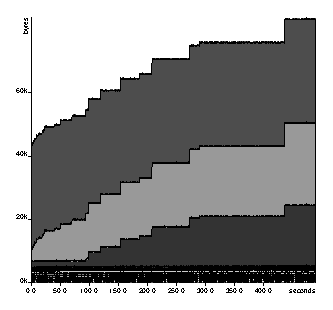
\includegraphics[width=\textwidth]{space/amis-orig.eps}
    \caption{Amicable Pairs}
    \label{fig:searchparty-examples-space:amis-orig}
  \end{subfigure}
  \begin{subfigure}{0.4\textwidth}
    \includegraphics[width=\textwidth]{space/amis-sp}
    \caption{Amicable Pairs (Search Party)}
    \label{fig:searchparty-examples-space:amis-sp}
  \end{subfigure}

  % \begin{subfigure}{0.4\textwidth}
  %   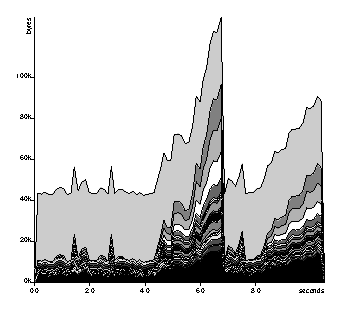
\includegraphics[width=\textwidth]{space/mate-orig}
  %   \caption{Mate-in-N}
  %   \label{fig:searchparty-examples-space:mate-orig}
  % \end{subfigure}
  % \begin{subfigure}{0.4\textwidth}
  %   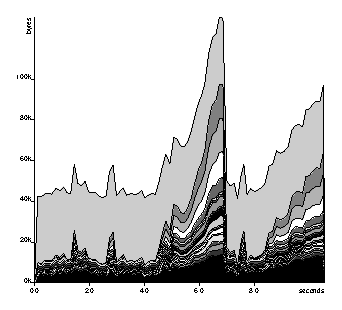
\includegraphics[width=\textwidth]{space/mate-sp}
  %   \caption{Mate-in-N (Search Party)}
  %   \label{fig:searchparty-examples-space:mate-sp}
  % \end{subfigure}

  \begin{subfigure}{0.4\textwidth}
    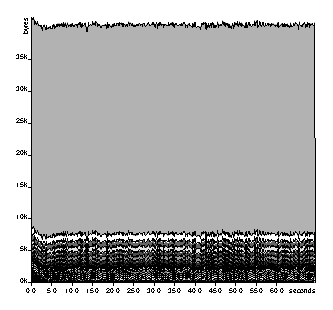
\includegraphics[width=\textwidth]{space/sols-orig}
    \caption{sols}
    \label{fig:searchparty-examples-space:sols-orig}
  \end{subfigure}
  \begin{subfigure}{0.4\textwidth}
    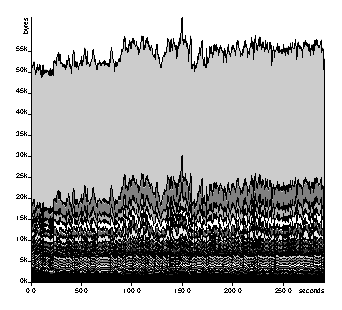
\includegraphics[width=\textwidth]{space/sols-sp}
    \caption{sols (Search Party)}
    \label{fig:searchparty-examples-space:sols-sp}
  \end{subfigure}

  \begin{subfigure}{0.4\textwidth}
    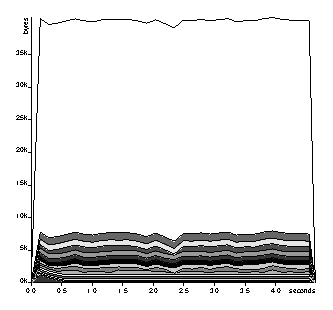
\includegraphics[width=\textwidth]{space/sols2-orig}
    \caption{sols'}
    \label{fig:searchparty-examples-space:sols2-orig}
  \end{subfigure}
  \begin{subfigure}{0.4\textwidth}
    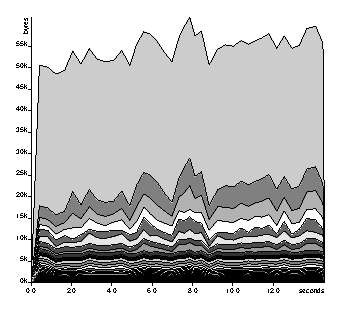
\includegraphics[width=\textwidth]{space/sols2-sp}
    \caption{sols' (Search Party)}
    \label{fig:searchparty-examples-space:sols2-sp}
  \end{subfigure}

  % \begin{subfigure}{0.4\textwidth}
  %   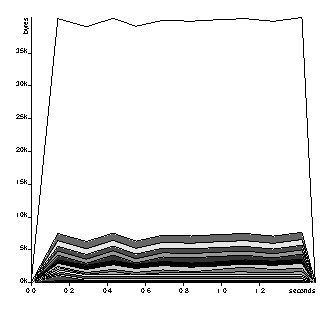
\includegraphics[width=\textwidth]{space/sols3-orig}
  %   \caption{sols''}
  %   \label{fig:searchparty-examples-space:sols3-orig}
  % \end{subfigure}
  % \begin{subfigure}{0.4\textwidth}
  %   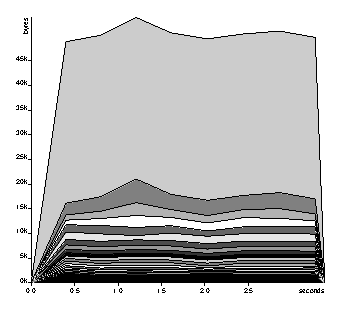
\includegraphics[width=\textwidth]{space/sols3-sp}
  %   \caption{sols'' (Search Party)}
  %   \label{fig:searchparty-examples-space:sols3-sp}
  % \end{subfigure}

  % \begin{subfigure}{0.4\textwidth}
  %   \includegraphics[width=\textwidth]{space/iso-orig}
  %   \caption{Iso. Checker}
  %   \label{fig:searchparty-examples-space:iso-orig}
  % \end{subfigure}
  % \begin{subfigure}{0.4\textwidth}
  %   \includegraphics[width=\textwidth]{space/iso-sp}
  %   \caption{Iso. Checker (Search Party)}
  %   \label{fig:searchparty-examples-space:iso-sp}
  % \end{subfigure}

  \caption{Benchmark memory results, with the Search Party version
    executed with 4 threads.}
  \label{fig:searchparty-examples-space}
\end{figure*}

\subsection*{Amicable Pairs}
\label{sec:searchparty-examples-amis}

An \textit{amicable pair} is a pair of numbers such that the sum of
the proper divisors of each equals the other. For example, $(220,
284)$ is an amicable pair, as we have:

\begin{align*}
  D(220) &= \left\{1,~2,~4,~5,~10,~11,~20,~22,~44,~55,~110\right\}\\
  D(284) &= \left\{1,~2,~4,~71,~142\right\}\\
  220    &= 1 + 2 + 4 + 71 + 142\\
  284    &= 1 + 2 + 4 + 5 + 10 + 11 + 20 + 22 + 44 + 55 + 110
\end{align*}

Where $D(x)$ here is the set of proper divisors of $x$. This benchmark
enumerates and prints the first 100 amicable pairs. We can enumerate
the set of amicable pairs with a list comprehension:

\begin{minted}{haskell}
amicablePairs :: [(Integer, Integer)]
amicablePairs =
  [ (n, sn)
  | n <- [2..]
  , let sn = sigmaBar n
  , sn > n
  , sigmaBar sn == n]
\end{minted}

\noindent where \verb|sigmaBar| computes this divisor sum. To avoid
duplication, the elements of each pair are in ascending order.

Initially pairs are found very quickly, but the pace of enumeration
slows towards the end. As \verb|amicablePairs| is a generate-and-test
computation with a simple generator and a more complex test, we aim to
derive a new version using Search Party.

We can obtain it by a fairly mechanical translation of the original:

\begin{enumerate}
  \item Split the implicit \verb|filter| out of the comprehension,
\begin{minted}{haskell}
amicablePairs =
  filter (\(n,sn) -> sn > n && sigmaBar sn == n)
  [(n,sigmaBar n) | n <- [2..]]
\end{minted}

  \item Factor out the predicate,
\begin{minted}{haskell}
amicablePairs =
  filter ami [(n,sigmaBar n) | n <- [2..]]
  where
  ami (n, sn) = sn > n && sigmaBar sn == n
\end{minted}

  \item Turn the \verb|filter| into an \verb|inOrder|,
\begin{minted}{haskell}
amicablePairs =
  inOrder ami [(n,sigmaBar n) | n <- [2..]]
  where
  ami (n, sn) = sn > n && sigmaBar sn == n
\end{minted}

  \item Replace \verb|inOrder| with \verb|>!|, which is just
    \verb|flip inOrder|,
\begin{minted}{haskell}
amicablePairs =
  [(n,sigmaBar n) | n <- [2..]] >! ami
  where
  ami (n, sn) = sn > n && sigmaBar sn == n
\end{minted}

  \item Convert the \verb|Stream| back into a list,
\begin{minted}{haskell}
amicablePairs =
  toList $ [(n,sigmaBar n) | n <- [2..]] >! ami
  where
  ami (n, sn) = sn > n && sigmaBar sn == n
\end{minted}
\end{enumerate}
%$

This final version isn't too dissimilar to the \verb|filter| version
in step 2. In fact, we could have stopped in step 3, had we added a
call to \verb|toList| as well. As can hopefully be seen, for list
comprehensions with a single generator, the introduction of
parallelism is quite simple.

\begin{figure}[t]
  \centering
  \begin{tabularx}{\linewidth}{|X|X|X|X|}
    \hline \textbf{Version} & \textbf{Optimum} & \textbf{Actual} & \\
    \hline -N1  & 179s (1x)   & 222s (0.8x)  & 0.8x \\
           -N2  & 89.5s (2x)  & 134s (1.3x)  & 0.7x \\
           -N4  & 44.8s (4x)  & 72.1s (2.5x) & 0.6x \\
           -N8  & 22.4s (8x)  & 39.2s (4.6x) & 0.6x \\
           -N16 & 11.2s (16x) & 28.6s (6.3x) & 0.4x \\
           -N24 & 7.5s  (24x) & 26.8s (6.7x) & 0.3x \\
    \hline
  \end{tabularx}
  \caption{Optimal speed-ups for Amicable Pairs}
  \label{fig:searchparty-examples-amis-amdahl}
\end{figure}

Figure \ref{fig:searchparty-examples-amis-amdahl} shows optimal
speed-ups for this benchmark, calculated using Amdahl's law after
profiling revealed a negligible proportion of overall execution time
sequentially consuming the list. The entire \verb|amicablePairs|
comprehension, rather than just the explicit tests, was profiled. Due
to lazy evaluation, parallelisation of the test also parallelises the
generation to some extent.

\subsection*{Mate-in-N}
\label{sec:searchparty-examples-mate}

The applicability of Search Party depends on the overall structure of
a computation including a generate-and-test search. There is some
sequential prefix doing some set-up, a period amenable to parallelism,
and then a sequential suffix producing the final result. Ideally, the
sequential prefix and suffix are very small compared to the parallel
middle. This was certainly the case in the Amicable Pairs example.

In the Mate-in-N benchmark, the prefix and suffix computations are
more significant. This program attempts to solve the Mate-in-N
problem. A chess position is presented where one side can mate the
other in $n$ moves. The challenge is to find a pruned game-tree
demonstrating the win no matter what moves the opponent makes. Here is
an example input to the program (a position that actually arises in
Kohtz v. Kockelkorn, 1875):

\begin{verbatim}
- - - - - - - K 
- - - - - - - - 
- - - - - n - p 
- - - - - - - - 
- - - - - - - - 
- - - - - B P - 
- - - - - - - - 
b - - - - - k - 

White to move and mate in 5
\end{verbatim}

Due to differing difficulties, timing results were averaged over 10
different problems.

The program is structured as generating a game tree, which can be done
in parallel, but then pruning it sequentially to produce a minimal
tree.

The introduction of parallelism is a little more complex than in the
Amicable Pairs, using an additional function parameter to prevent
nested parallelism, which Search Party currently does not cope well
with.

The original definition

\begin{minted}{haskell}
solution :: Board -> Colour -> Int -> Maybe Solution
solution bd c n | n > 0 = 
  let mds = moveDetailsFor c bd
  in foldr solnOr Nothing mds
\end{minted}

\noindent is altered as follows.

\begin{minted}{haskell}
solution :: Bool
         -> Board -> Colour -> Int -> Maybe Solution
solution top bd c n | n > 0 = 
  let mds = moveDetailsFor c bd
  in if top
     then toMaybe $ mds .? (flip solnOr Nothing)
     else foldr solnOr Nothing mds
\end{minted}
%$

The \verb|top| parameter indicates whether this is a ``top-level
search'', or a search begun when constructing some lower level of the
game tree. The candidate solutions for parallel exploration correspond
to the possible initial moves.

\begin{figure}[t]
  \centering
  \begin{tabularx}{\linewidth}{|X|X|X|X|}
    \hline \textbf{Version} & \textbf{Optimum} & \textbf{Actual} & \\
    \hline -N1  & 20.9s (1.0x) & 21.3s (1.0x) & 1.0x \\
           -N2  & 11.6s (1.8x) & 11.5s (1.8x) & 1.0x \\
           -N4  & 6.9s (3.0x)  & 7.8s (2.7x)  & 0.8x \\
           -N8  & 4.6s (4.6x)  & 6.4s (3.3x)  & 0.7x \\
           -N16 & 3.4s (6.2x)  & 6.5s (3.2x)  & 0.5x \\
           -N24 & 3.0s (7.0x)  & 7.0s (3.0x)  & 0.4x \\
    \hline
  \end{tabularx}
  \caption{Optimal speed-ups for Mate-in-N}
  \label{fig:searchparty-examples-mate-amdahl}
\end{figure}

Figure \ref{fig:searchparty-examples-mate-amdahl} shows optimal
speed-ups for this benchmark, assuming that 89.4\% of the work could
be parallelised. This is optimistic, as it assumes every (recursive)
call to \verb|solution| could be executed in parallel. Search Party is
not suitable for expressing this sort of recursive generation of new
work, as it does not currently share worker threads. As the result of
the computation is finite and used in full, the Par monad may be a
more viable approach here.

\subsection*{Hutton's Countdown Solver}
\label{sec:searchparty-examples-hutton}

\textit{Countdown} is a gameshow where one of the components is a
number game. Contestants choose a collection of 6 number cards, and
then must get as close as possible to a randomly-generated three-digit
number using only addition, subtraction, multiplication, and
division. Not all numbers must be used, a number may be used as many
times as it appears on the chosen number cards, and all stages of the
calculation must involve integer values.

Graham Hutton produced a series of programs\footnote{Timing results
  for only the most optimal are shown.} to solve the
\textit{Countdown} numbers game\cite{hutton}, with different levels of
intelligence in how the problem was approached. The simplest is just a
brute-force generation of all possible legal expressions; then there
is a version which eliminates invalid solutions more rapidly; and
finally there is a version exploiting arithmetical properties.

The key elements of the three programs are list comprehensions, and
are as follows,

\begin{minted}{haskell}
sols, sols', sols'' :: [Int] -> Int -> [Expr]
sols ns n   = [e | ns' <- choices ns
                 , e   <- exprs   ns'
                 , eval e == [n]]

sols' ns n  = [e | ns'   <- choices ns
                 , (e,m) <- results ns'
                 , m == n]

sols'' ns n = [e | ns'   <- choices  ns
                 , (e,m) <- results' ns'
                 , m == n]
\end{minted}

Where \verb|Expr| is an ADT representing expressions composed of the
operators legal in the game.

One hundred random \verb|(input, target)| pairs were generated, and
the following benchmark constructed,

\begin{minted}{haskell}
main :: IO ()
main = mapM_ (print . length . uncurry solutions) ...
\end{minted}

Timing results are divided by 100, to represent the time taken to
solve an ``average'' \textit{Countdown} challenge.

Parallelising the na\"{\i}ve solution proved to be a little tricky. A
fairly straightforward transformation would be something like:

\begin{minted}{haskell}
sols ns n = parFilter (\e -> eval e == [n]) .
  concatMap exprs $ choices ns
\end{minted}
%$

\noindent where \verb|parFilter| is a function built out of the pieces
we have seen so far. Unfortunately, this performed poorly, and
contention over the list of expressions seemed to be the
problem.

Another version constructs the lists in separate threads and
concatenates at the end.

\begin{minted}{haskell}
sols ns n = concat . parMap go $ choices ns where
  go ns' = [e | e <- exprs ns', eval e == [n]]
\end{minted}
%$

Here \verb|parMap| is defined to evaluate each element of the result
to weak-head normal form, to ensure work is being done in
parallel. This performed better, but still rather slowly. The problem
with this sort of approach is that if any empty lists are produced, we
will waste time concatenating them at the end, sequentially. It would
be preferable to discard empty results in parallel.

This observation lead to a final version:

\begin{minted}{haskell}
sols ns n = concat . go $ choices ns where
  go xs = toList $ xs >? (check . es)
  es ns' = [e | e <- exprs ns', eval e == [n]]

  check [] = Nothing
  check xs = Just xs
\end{minted}

Now, if a choice produces an empty list of expressions, it is
discarded, we only concatenate nonempty lists, and so no time is
wasted on useless results after the parallel computation finishes.

In addition to providing a collection of ``primitive'' functions to
parallelise in terms of \verb|Find| and \verb|Stream|, a part of the
goal of Search Party is to be easy to integrate into existing code.
So functions like \verb|parMap|, \verb|parFilter|, and
\verb|parConcatMap| have been included in the library, to help
approach this goal.

With the insight that the generation of results from choices had to
happen in the parallel threads, producing parallel variants of the two
optimised functions was simple,

\begin{minted}{haskell}
sols'  ns n = parConcatMap
  (\ns' -> [e | (e,m) <- results  ns', m == n]) $
  choices ns

sols'' ns n = parConcatMap
  (\ns' -> [e | (e,m) <- results' ns', m == n]) $
  choices ns
\end{minted}

\begin{figure}[t]
  \centering
  \begin{tabularx}{\linewidth}{|X|X|X|X|}
    \hline \textbf{Version} & \textbf{Optimum} & \textbf{Actual} & \\
    \hline -N1  & 0.49s (1.0x) & 0.55s (0.9x) & 0.9x \\
           -N2  & 0.25s (1.9x) & 0.35s (1.4x) & 0.7x \\
           -N4  & 0.14s (3.6x) & 0.21s (2.3x) & 0.6x \\
           -N8  & 0.08s (6.4x) & 0.16s (3.1x) & 0.5x \\
           -N16 & 0.04s (10x)  & 0.16s (3.1x) & 0.3x \\
           -N24 & 0.04s (13x)  & 0.18s (2.7x) & 0.2x \\
    \hline
  \end{tabularx}
  \caption{Optimal speed-ups for Hutton's Countdown solver}
  \label{fig:searchparty-examples-hutton-amdahl}
\end{figure}

Figure \ref{fig:searchparty-examples-hutton-amdahl} shows optimal
speed-ups for this benchmark, assuming all of the work done in the
\verb|exprs|, \verb|eval|, \verb|results| and \verb|results'|
functions can be parallelised. As with the Mate-in-N problem, this is
optimistic, due to the lazy evaluation of the rest of the
comprehension.

\subsection*{Isomorphism Checker}
\label{sec:searchparty-examples-isos}

GP2\cite{gp2} is a nondeterministic programming language based on
graph transformation, and an important component of the reference
interpreter is a program to check if two graphs are isomorphic. The
isomorphism checker first checks that the graphs are the same size,
and then searches for an isomorphism by generating candidate node
morphisms respecting node labels and degrees, testing if a morphism is
a bijection.

The GP2 graph file format is very simple, and by permuting the list of
nodes, different but isomorphic graphs can be produced. 100 random
permutations of a graph containing (disjoint) Sierpinski order 2 and 3
graphs were produced, with timing results averaged over this.

The introduction of parallelism is quite simple:

\begin{minted}{haskell}
isomorphic :: (Ord a, Ord b)
           => Graph a b -> Graph a b -> Bool
isomorphic g1 g2 =
  length ns1 == length ns2 &&
  ( parAny
    (edgesIso g1 g2)
    (bijectionsWith (nodeAttribs g1) ns1
                    (nodeAttribs g2) ns2)
  )
  where
  ns1 = allNodeKeys g1
  ns2 = allNodeKeys g2
\end{minted}

The introduction of a \verb|parAny| (in place of a regular \verb|any|)
is the only change made. As can be seen in Figure
\ref{fig:searchparty-examples-time} performance begins to fall with
more than 4 parallel workers. It is possible that a more sophisticated
introduction of parallelism could have yielded better results, but
this was not pursued.

\begin{figure}[t]
  \centering
  \begin{tabularx}{\linewidth}{|X|X|X|X|}
    \hline \textbf{Version} & \textbf{Optimum} & \textbf{Actual} & \\
    \hline -N1  & 1.7s  (1.0x) & 2.27s (0.7x) & 0.7x \\
           -N2  & 0.91s (1.9x) & 1.51s (1.1x) & 0.6x \\
           -N4  & 0.52s (3.3x) & 0.78s (2.2x) & 0.7x \\
           -N8  & 0.33s (5.3x) & 1.33s (1.3x) & 0.2x \\
           -N16 & 0.22s (7.6x) & 5.61s (0.3x) & 0.03x \\
           -N24 & 0.19s (8.9x) & 8.31s (0.2x) & 0.02x \\
    \hline
  \end{tabularx}
  \caption{Optimal speed-ups for the Isomorphism Checker}
  \label{fig:searchparty-examples-isos-amdahl}
\end{figure}

Figure \ref{fig:searchparty-examples-isos-amdahl} shows optimal
speed-ups for this benchmark. The results for $n \geq 8$ are
poor. Looking at the source of \verb|bijectionsWith|, it appears to be
very sequentially in its current incarnation. This imposes unnecessary
sequentiality and blocking when claiming work items, and so much of
the benefit of parallelism is lost.

\section{Related Work}
\label{sec:searchparty-related}

Speculative computation\cite{spec} is, in some sense, the exact
opposite of lazy evaluation. Whereas in most cases, we wish to delay a
computation until its result is demanded, sometimes it can be worth
computing something ahead of time, on the assumption that it is likely
to be needed. Such efforts will be wasted if the assumption proves
incorrect. The cost of \textit{speculating} on such results can be
lessened by performing the evaluation in parallel with the main thread
of control, giving a net gain if the assumption is correct.

GUM\cite{gum} introduces speculative parallelism in Haskell with the
\verb|par| combinator, which starts evaluating its first argument in
parallel and returns its first, and demonstrates a speed-up even with
this primitive operation alone. In contrast, Search Party uses much
more controlled parallelism, with control of the scheduling taken from
the runtime system. This prevents a risk of a large amount of parallel
computation being started at once, which would increase resource
contention, which could happen with liberal application of \verb|par|.

One application of speculative parallelism in Haskell is the work of
Cope, Gent, and Hammond on parallel heuristic search\cite{parsat}
applied to SAT solvers. In this work they produce two sequential SAT
solvers which would be amenable to parallelism, rather than attempt to
produce an optimal sequential solver. Both algorithms include a
splitting step, to turn a problem into two simpler cases. Relative
speed-ups of between 0.92 and 4.8 are obtained by introduction of
parallelism at this splitting step.

A version with explicit speculation support, where the parallel
computation returns a continuation if it executes for too long without
finding a result, performs slightly worse than the naive, more eager,
approach. The authors suggest this may be due to overhead in their
implementation of this mechanism.

The Strategies\cite{strategies} library provides for speculative
computation in Haskell by allowing the programmer to write an
\textit{evaluation strategy}, specifying how some data structure is to
be evaluated. Such strategies may include, for example, evaluating
elements of a list in parallel. The building blocks are \verb|rseq|,
which forces sequential evaluation, and \verb|rpar|, which forces
parallel evaluation.

The \verb|Stream| combinators of Search Party are very much in a
speculative style: values not yet requested by the programmer are
being searched for in parallel, on the assumption that they are
\textit{likely} to be needed. Unlike Strategies, the parallelism is
much more precisely controlled: the number of parallel agents is
fixed, and the agents block if results are not demanded. The
\verb|Stream| combinators can be thought of as variants on a parallel
\verb|mapMaybe| operation, which could be implemented na\"{\i}vely
with Strategies as follows.

\begin{minted}{haskell}
import Control.Parallel.Strategies
parMapMaybe :: (a -> Maybe b) -> [a] -> [b]
parMapMaybe f = catMaybes . parMap rseq f
\end{minted}

However the Strategies \verb|parMap| sparks off each element of the
list at once, resulting in a potentially huge degree of
parallelism. This in turn can lead to more contention over resources,
and lowered performance. A work-around, then, might be to introduce
chunking,

\begin{minted}{haskell}
parMapMaybe f = withStrategy (parListChunk 16 rseq)
              . map f
\end{minted}

But what should the chunk size be? Furthermore, with an infinite list,
this will still result in a great number of sparks. As there is no way
to check if a value has been evaluated, there is no way for the
programmer to keep the number of parallel agents constant, or to pause
work if the agents are producing new results significantly more
quickly than they are being demanded.

The \verb|Par| monad\cite{par} provides for deterministic parallelism,
and so might be seen as an obvious candidate to use, rather than the
deterministic \verb|Find| and \verb|Stream| combinators. However, as
noted, relaxing the requirement of determinism can be faster in some
cases.

Gaining a speed-up with parallelism necessarily requires doing work in
separate threads, which laziness can thwart. The \verb|Par| monad is
fully strict by default. Using Search Party to map a function over a
list in parallel requires careful forcing of values. For example, the
\verb|parMap| and \verb|parConcatMap| functions evaluate results to
WHNF in parallel. This sadly means that the convenience functions
provided in Search Party are \textit{not} a drop-in replacement for
the standard list-processing functions in the presence of $\bot$s, as
can be seen in this simple example:

\begin{minted}{haskell}
bad = null . parMap (\_ -> last [1..])
\end{minted}

Here, \verb|bad [1,2,3]| is $\bot$, whereas if \verb|map| were used
instead, the result would be \verb|False|.

Perhaps nondeterminism is over-rated. Most programmers would only use
a library like Search Party to parallelise list comprehensions and
similar pure computations. Even here, the \verb|Par| monad may not be
suitable, as when a \verb|Par| computation terminates, all parallelism
must be complete, consider:

\begin{minted}{haskell}
import Control.Monad.Par
parMapMaybe f = catMaybes . runPar . parMap f
\end{minted}

This \verb|parMap| function spawns one thread for every element of the
list, but as we \textit{do} know if a thread has finished with
\verb|Par|, we can rewrite this to refrain from spawning new threads
until they are needed. The problem is that no such function will
terminate until the \textit{entire} list has been processed. In the
case of an infinite list, then, the result is $\bot$.

\section{Conclusions}
\label{sec:searchparty-concs}

We have presented a new library for parallel generate-and-test style
computations, and demonstrated that it can give a significant speed-up
over the sequential case. Furthermore, we have shown that it is not
feasible to achieve the same flexibility as Search Party with
Strategies or the \verb|Par| monad.

Parallelism and concurrency are generally seen as worthwhile tools to
apply to large problems. Because of the difficulty of correctly using
them, applying them to small problems is often simply not
considered. However, we have shown here that this ``parallelism in the
small'' \textit{can} and \textit{does} offer improved performance, and
so should be considered also.

Concurrent Search Party computations currently receive no special
treatment. Worker threads are created for all computations, and may
contend over execution time. This can be seen in the applicative
instance for \verb|Find|, but also arises with nested Search Party
computations. A solution worth pursuing would have a global pool of
workers which all computations share.


\printbibliography

\end{document}
